\documentclass[a4paper,12pt]{ThesisStyle}
\usepackage[utf8]{inputenc}
\usepackage{thesis-style}
\usepackage{parskip}
\usepackage{beramono}
\usepackage[section]{placeins}
\usepackage{tabularx}
\usepackage{float}
\usepackage{xcolor}
\usepackage{colortbl}
\usepackage[labelfont=bf]{caption}
\usepackage{booktabs}
\usepackage{array}
\usepackage{graphicx, adjustbox}
\usepackage{tikz}
\usepackage{pdflscape}

\usetikzlibrary{positioning}

\tikzset{main node/.style={circle,fill=blue!20,draw,minimum size=1cm,inner sep=0pt},}

\setlength{\headheight}{14.49998pt}
\addtolength{\topmargin}{-0.89998pt}

\definecolor{TblDef}{HTML}{FFFFE6}
\definecolor{Gray}{HTML}{E2E2E2}
\definecolor{Green}{HTML}{D5E8D4}
\definecolor{Blue}{HTML}{DAE8FC}
\definecolor{Orange}{HTML}{FFE6CC}
\definecolor{Purple}{HTML}{E1D5E7}

\renewcommand\tabularxcolumn[1]{m{#1}}

\AtBeginDocument{
\hypersetup{pdftitle=Eina de suport per a l'elaboració dels horaris dels graus de l'EPS}
\hypersetup{pdfauthor=Adrià Ribas Chico}
}

\begin{document}

\newgeometry{margin=1in}
\begin{titlepage}

\setlength{\parskip}{0pt}

\begin{center}

\includegraphics[width=0.65\textwidth]{assets/logos/EPS_centrat.png}

\vspace{2cm}

{\Large Grau en Enginyeria Informàtica\par}
\vspace{0.2cm}
\vspace{3.5cm}
\textsc{\Large Projecte Final de Grau}
\vspace{0.2cm}

\begin{center}
  \rule{\textwidth}{0.05cm}
\end{center}
\vspace{0.15cm}
{\huge \bfseries Eina de suport per a l'elaboració dels horaris dels graus de l'EPS\par}
\vspace{0.4cm}
\begin{center}
  \rule{\textwidth}{0.05cm}
\end{center}

\vspace{1cm}
 
\begin{minipage}[t]{0.4\textwidth}
\begin{flushleft}
    \large
    \emph{Autor:}\\
    Adrià Ribas Chico
\end{flushleft}
\end{minipage}
\begin{minipage}[t]{0.45\textwidth}
\begin{flushright} 
    \large
    \emph{Tutors:} \\
    Dra. Marta Fort Masdevall \\
    Dr. Antonio Rodríguez Benítez
\end{flushright}
\end{minipage}

\vspace{1.2cm}

\textsc{\Large Memòria}

\vspace{1.2cm}

{\large
Convocatòria:\\
Gener de 2023

\vspace{0.9cm}

Departament:\\
Informàtica, Matemàtica Aplicada i Estadística\\
}
\vfill
\end{center}
\end{titlepage}
\restoregeometry

\thispagestyle{empty}
\vspace*{\fill}

{\bfseries  \Large }
\vspace{0.75cm}

\begin{footnotesize}

  \begin{flushleft} 
    \begin{tabular}{ @{}lp{0.4\textwidth}@{} } 
    \emph{Projecte:}  & Projecte Final de Grau\\ 
    \emph{Document:}  & Memòria\\ 
    \emph{Títol}:    & Eina de suport per a l'elaboració dels horaris dels graus de l'EPS\\
    \emph{Autor}:   & Adrià Ribas Chico\\
    \emph{Data}:     & 10 de gener de 2023\\
    
    \end{tabular}
    \end{flushleft}
    
    \vspace{0.75cm}
    
    
    \begin{minipage}[t]{\textwidth}
      \begin{flushleft} 
        \emph{Estudi:}\\
        Grau en Enginyeria Informàtica\\
        \href{https://www.udg.edu}{Universitat de Girona}
      \end{flushleft}
    \end{minipage}
    
    \vspace{0.75cm}
    
    \begin{minipage}[t]{0.5\textwidth}
      \begin{flushleft} 
        \emph{Tutora 1:}\\
        Dra. Marta Fort Masdevall\\
        Universitat de Girona\\
        Informàtica, Matemàtica Aplicada i Estadística\\
        \href{mailto:marta.fort@udg.edu}{marta.fort@udg.edu}
      \end{flushleft}
    \end{minipage}
    
    \begin{minipage}[t]{0.5\textwidth}
      \begin{flushleft} 
        \emph{Tutor 2:}\\
        Dr. Antonio Rodríguez Benítez\\
        Universitat de Girona\\
        Informàtica, Matemàtica Aplicada i Estadística\\
        \href{mailto:antonio.rodriguez@udg.edu}{antonio.rodriguez@udg.edu}
      \end{flushleft}
    \end{minipage}

\end{footnotesize}

\let\cleardoublepage\clearpage
\pagenumbering{roman}
\frontmatter
\dominitoc

\chapter*{Agraïments}
\label{cap:agraiments}

Agraïments \ldots


\tableofcontents
\listoffigures
\listoftables

\pagenumbering{gobble}
\mainmatter

\chapter{Introducció}
\label{cap:intro}

\section{Antecedents}
\label{sec:antecedents}

En aquesta secció, es resumiran els antecedents que han donat peu al plantejament d'aquest projecte.

La idea del projecte neix de determinades necessitats que cert personal de l'Escola Politècnica Superior de la Universitat de Girona fa temps que té. Més concretament, es tracta d'una necessitat del personal encarregat de gestionar tot el que fa referència a la confecció i manteniment dels horaris del centre: horaris dels estudis, dels professors, ocupació d'aules i espais, etc.

Actualment, en els processos d'elaboració dels horaris i de distribució de docència en professors hi intervenen més de quaranta persones, les quals utilitzen mètodes i eines incòmodes i poc àgils, a part de no estar automatitzades ni específicament dissenyades per abordar aquest tipus de tasques. Tampoc existeix cap plataforma que unifiqui les fases d'aquest procés de gestió ni que n'estableixi una manera de fer comuna.

No tenen manera de detectar incompatibilitats horàries ni solapaments \textit{a priori} de manera automàtica. Degut a això, en moltes ocasions s'han de repetir certes fases del procés fins que el resultat és vàlid i la gent implicada hi està d'acord.

Al capítol~\ref{cap:marcdetreball} es descriurà amb més profunditat com funcionen avui dia aquests processos d'elaboració i gestió d'horaris de l'escola.

\section{Propòsit}
\label{sec:proposit}

En aquesta secció, s'exposarà el propòsit general del projecte, tenint en compte els antecedents vists a la secció~\ref{sec:antecedents}.

En definitiva, la gestió dels horaris de l'EPS suposa una inversió de temps massa elevada per a la gent que se n'ocupa. És per això que Marta Fort Masdevall, coordinadora d'estudi del Grau en Enginyeria Informàtica de la universitat, proposa un projecte de fi de grau pensat per a dues persones que té la finalitat de trobar una solució al problema.

El propòsit és desenvolupar una eina de suport informàtic que permeti a l'usuari elaborar horaris de forma àgil, eficient i segura. L'eina també hauria de ser capaç de comprovar automàticament la disponibilitat de les aules, les incompatibilitats horàries dels professors i la concordança entre les assignatures i el nombre de grups previstos. A més a més, hauria d'oferir diverses vistes per tal que l'usuari pugui visualitzar la informació, com ara:
\begin{itemize}
  \item Els horaris d'un estudi per curs i quadrimestre.
  \item Els horaris d'un professor per quadrimestre.
  \item L'ocupació d'un espai per quadrimestre.
\end{itemize}

També es planteja la possibilitat de disposar d'un sistema de control d'usuaris. Cada usuari tindria assignat un conjunt de rols determinat. Els rols representarien els diferents càrrecs del personal de l'EPS en matèria de gestió d'horaris. Així doncs, cada usuari podria executar les accions i consultar la informació que el seu conjunt de rols li permeti. D'aquesta manera, es dividirien les diferents tasques i processos entre rols d'usuari i cadascun dels càrrecs podria realitzar la feina que li correspon. La proposta inicial comprèn els rols d'usuari següents:
\begin{itemize}
  \item \texttt{Administrador}: Introdueix les dades dels plans docents i dóna d'alta Coordinadors i Directors de departament.
  \item \texttt{Coordinador}: Elabora els horaris.
  \item \texttt{Director de departament}: Dóna d'alta Responsables de docència.
  \item \texttt{Responsable de docència}: Dóna d'alta i assigna Professors als grups.
  \item \texttt{Professor}: Visualitza el seu horari.
\end{itemize}

A més a més, l'aplicació hauria de ser accessible via web. D'aquesta manera, tots els usuaris podrien utilitzar-la des de qualsevol lloc i dispositiu, sense preocupar-se d'instal·lacions ni actualitzacions.

\section{Motivacions}
\label{sec:motivacions}

En aquesta secció, es parlarà en primera persona sobre quines motivacions personals hi ha darrere del projecte i en justifiquen l'elecció.

Un dels aspectes que més em motiven de la informàtica en general és el fet de poder ajudar la gent a estalviar el seu temps, el qual té un gran valor. En moltes ocasions, una persona, un grup o fins i tot una institució, inverteix una quantitat elevada de temps en realitzar certes accions o activitats, sigui en l'àmbit que sigui. Aquest temps es pot reduir si l'acció o activitat en qüestió té una part suficientment mecànica. Tanmateix, encara que no la tingui, sovint és possible desenvolupar una eina informàtica que n'augmenti l'eficiència o, si més no, dinamitzar-la i fer que resulti més còmoda i pràctica.

D'aquí sorgeix el meu objectiu principal pel que fa a la informàtica, que és precisament aportar el meu gra de sorra a aquesta causa.

Per aquest motiu, m'ha cridat molt l'atenció la proposta d'aquest projecte. És una molt bona oportunitat per contribuir a millorar el procés de gestió i elaboració d'horaris de l'escola, que sol resultar bastant costós en temps per a les persones que hi participen.

D'altra banda, em motiva molt el fet de desenvolupar una aplicació que podrà ser implantada en un entorn real i que podrà beneficiar les persones que la facin servir. No em cridaria tant dur a terme un altre projecte que, un cop finalitzat, fos simplement arxivat, sense utilitat pràctica per a ningú més excepte per a mi, que seria l'únic que me'n beneficiaria, ja que igualment obtindria coneixements i experiència.

Actualment i cada vegada més, m'interessa el desenvolupament d'entorns web. És per això que un factor decisiu a l'hora d'escollir aquesta proposta de PFG ha estat que un dels requisits sigui desenvolupar-lo en format de plataforma web.

Per últim, m'agradaria afegir que, per motius d'ambició i d'obtenció més àmplia de coneixements, he decidit dur a terme el projecte de manera individual, encara que estigui pensat per a dues persones. Fer-lo sol em portarà molt més temps, però permetrà no perdre'm cap detall de tot el que suposa desenvolupar una aplicació d'aquest estil.

\section{Objectius generals}
\label{sec:objectius_generals}

En aquesta secció, s'enumeraran els objectius generals del projecte, que ja s'han deixat entreveure prèviament a la secció~\ref{sec:proposit}. No obstant això, a continuació se'n presenta la llista completa:
\begin{itemize}
  \item Desenvolupar una plataforma o aplicació web que permeti dur a terme les tasques de gestió i elaboració dels horaris de l'EPS.
  \item Proporcionar unes interfícies d'usuari curosament dissenyades que siguin atractives, intuïtives, còmodes i, sobretot, eficients.
  \item Emmagatzemar i processar dinàmicament les dades i relacions referents als diversos estudis, cursos, quadrimestres, assignatures, grups, espais, professors, etc.
  \item Detectar automàticament i avisar de qualsevol tipus d'inconsistència o incompatibilitat horària, per tal d'aportar seguretat al treball.
  \item Possibilitar la pujada d'arxius externs de dades que serveixin per obtenir la informació bàsica necessària per al funcionament de l'aplicació.
  \item Permetre la visualització de l'ocupació de les aules, dels horaris dels professors i dels horaris de cada estudi, entre d'altres vistes que puguin ser d'utilitat pels usuaris.
  \item Admetre diferents rols d'usuari, als quals s'assigni una sèrie de tasques i un conjunt de permisos concret.
\end{itemize}

Cal remarcar que la finalitat de l'aplicació no és l'elaboració d'horaris i distribució de docència de manera automàtica. Per contra, el que es vol aconseguir és una eina específica que sigui de bon utilitzar i que permeti, gràcies a múltiples ajudes i automatitzacions, realitzar les tasques desitjades manualment.

A més a més, tampoc es preveu el llançament a producció de l'aplicació durant el projecte.

Un altre punt molt important a tenir en compte és que, degut a la magnitud dels objectius plantejats, s'ha decidit acotar-los lleugerament: tant la visualització de l'ocupació de les aules com la distribució de docència queden en un segon pla, encara que s'han de tenir molt en compte per tal de facilitar-ne una futura implementació. Això es justifica al capítol~\ref{cap:planificacio}, en què es conclou que la duració del projecte seria massa gran en cas de no acotar-lo.

Al capítol~\ref{cap:requisits} es desenvoluparan aquests objectius generals i es concretaran els requisits específics de l'aplicatiu. A més a més, se'n detallarà la prioritat que representen pel projecte.

\section{Estructura del document}
\label{sec:estructura_document}

En aquesta secció, es concretarà tant l'estructura del document com les desviacions que presenta respecte l'estipulat.

El document conté tots els capítols que s'estipulen a la \textit{Guia dels projectes final de grau de l'enginyeria informàtica}~\cite{GuiaPFG}.

No obstant això, presenta certes variacions pel que fa a l'ordre. De manera estàndard, els capítols 4, 5 i 6 han de ser, respectivament, ``Planificació'', ``Marc de treball i conceptes prèvis'' i ``Requisits del sistema''.

S'ha considerat que la comprensió del document milloraria si el marc de treball i els requisits es presentessin abans de la planificació, ja que, tant en els requisits com en la planificació, es fan servir la nomenclatura i els conceptes definits en el marc de treball. A més a més, la planificació s'ha realitzat a partir dels requisits.

Consegüentment, els capítols~\ref{cap:marcdetreball},~\ref{cap:requisits} i~\ref{cap:planificacio} d'aquest document són, respectivament, ``Marc de treball i conceptes prèvis'', ``Requisits del sistema'' i ``Planificació''.


\chapter{Estudi de viabilitat}
\label{cap:viabilitat}

\section{Viabilitat tecnològica}
\label{sec:viabilitat_tecnologica}

En aquesta secció, es valorarà si la realització del projecte és tècnicament viable.

Tal com s'ha explicitat al capítol~\ref{cap:intro}, el projecte no inclou el llançament a producció del programari. Per tant, com que tracta del desenvolupament d'una aplicació web, només fa falta un ordinador que disposi del \textit{software} necessari per executar-la, de manera local, en l'entorn de desenvolupament (veure capítol~\ref{cap:implantacio}).

\section{Costos de personal}
\label{sec:costos_personal}

En aquesta secció, es calcularan els costos relatius al personal que participa en el desenvolupament del projecte.

Com que el projecte tracta d'una aplicació web, és necessari diferenciar entre les persones que desenvolupen la part del servidor (\textit{back-end}) i les que desenvolupen la del client (\textit{front-end}).

Tal com es veurà al capítol~\ref{cap:estudi}, la tecnologia escollida per al \textit{back-end} és Node.js, mentre que l'escollida per al \textit{front-end} és Vue. Per tant, els preus que es tindran en compte als càlculs són els de desenvolupadors Node.js i desenvolupadors \textit{front-end} JavaScript en general.

A més a més, degut a la importància que prèn per al projecte el disseny de les interfícies d'usuari, cal comptar també amb dissenyadors d'interfícies.

A la taula~\ref{taula:costos_personal} es pot observar el detall de quina és l'aproximació dels costos de personal que suposaria el projecte. El valor dels sous s'ha obtingut de l'informe de salaris de la \emph{Guia HAYS 2022}~\cite{Hays}.

\begin{table}[H]
  \begin{tabularx}{\textwidth}{X  r  c  r}
    \toprule
    \rowcolor{TblDef}
    \textbf{Personal}                               & \textbf{Temps}      & \textbf{Preu}   & \textbf{Cost total} \\
    \midrule[0.9pt]
    Desenvolupadors Node.js                         & 315 hores           & 18.00 €/hora    & 5670.00 € \\
    \midrule
    Desenvolupadors \textit{front-end} JavaScript   & 440 hores           & 15.15 €/hora    & 6666.00 € \\
    \midrule
    Dissenyadors d'interfícies                      & 85 hores            & 14.68 €/hora    & 1247.80 € \\
    \midrule[0.9pt]
    \textbf{Total}                                  & \textbf{840 hores}  &                 & \textbf{13583.80 €} \\
    \bottomrule
  \end{tabularx}
  \caption{\label{taula:costos_personal} Taula de costos de personal.}
\end{table}

El temps de dedicació estimat dels diferents tipus de personal s'ha extret del capítol~\ref{cap:planificacio}. És important destacar que, per calcular els imports, s'ha fet servir el valor de temps total que comportaria el desenvolupament del 100\% del projecte, sense les acotacions marcades al capítol~\ref{cap:intro}.

Per últim, esmentar que el temps dedicat a la gestió del projecte s'ha tingut en compte per al càlcul del temps dels desenvolupadors.


\chapter{Metodologia}
\label{cap:metodologia}

\section{Gestió del projecte}
\label{sec:gestio_projecte}

En aquesta secció, s'abordaran els criteris seguits en quant a la gestió del projecte que s'han tingut en compte durant tot el seu cicle de vida.

La metodologia de gestió de projectes que s'ha seguit ha estat la que descriu PMBOK. PMBOK (\textit{Project Management Body of Knowledge})~\cite{PMBOK} és un llibre que recull un conjunt de terminologia estàndard, processos, bones pràctiques i directrius per a la gestió de projectes. No està restringit ni enfocat a la gestió de projectes d'una àrea en concret, sinó que és bastant genèric.

PMBOK és considerat un gran estàndard pel que fa a la gestió de projectes. Actualment, la majoria de projectes que es duen a terme el segueixen, ja que el fet que sigui tan genèric dóna peu al sorgiment de metodologies de desenvolupament més específiques que l'apliquen i s'hi basen.

D'acord amb PMBOK, el procediment general a seguir a l'hora de desenvolupar un projecte consta de les cinc fases següents:
\begin{enumerate}
  \item \texttt{Iniciació:} moment en què es planteja un problema que requereix una solució. Es defineix en què consistirà el projecte i se n'estudiarà la viabilitat per tal de decidir si tirar-lo endavant.
  \item \texttt{Planificació:} etapa en què es posen en manifest els objectius que persegueix el projecte i es planifica.
  \item \texttt{Execució:} recerca i aplicació de solucions que permetin implementar el projecte i satisfer-ne els objectius.
  \item \texttt{Seguiment i control:} fase que, normalment, s'executa simultàniament amb l'anterior. Permet controlar i regular el progrés del projecte, anticipar-se a problemes i aprofitar noves oportunitats.
  \item \texttt{Tancament:} finalització del projecte. Es comprova que realment se n'hagin assolit els objectius i es presenta als interessats.
\end{enumerate}

\section{Metodologia de desenvolupament}
\label{sec:metodologia_desenvolupament}

En aquesta secció, es descriurà quina ha estat la metodologia de desenvolupament que s'ha adoptat a l'hora de planificar i desenvolupar el projecte.

D'entrada, degut a que el projecte és individual, s'han descartat les metodologies AGILE, com ara SCRUM, encara que també siguin útils per a projectes individuals, no s'ha considerat necessària la seva aplicació. Per contra, s'ha optat per una estructuració en paquets de treball anomenada WBS que descriu el propi PMBOK.

WBS (\textit{work-breakdown structure}) és una tècnica o metodologia de desenvolupament basada en la descomposició jeràrquica d'un projecte en el que s'anomenen ``paquets de treball''. Cada paquet de treball ha de contenir, com a mínim, un identificador, nom, descripció, conjunt de tasques, temporalització i lliurable (més informació al capítol~\ref{cap:planificacio}). Si no és possible o resulta molt difícil la definició de la temporalització i tasques d'un paquet de treball, significa que es pot i s'ha de descomposar en subpaquets.

Pel que fa al seguiment del projecte, els aspectes que s'han anat desenvolupant han estat revisats pels tutors i valorats en conjunt. S'han realitzat reunions telemàtiques quan s'ha cregut necessari o s'han hagut de pendre algunes decisions importants, revisar i valorar algun aspecte o resoldre dubtes.


\chapter{Marc de treball i conceptes previs}
\label{cap:marcdetreball}

\section{Introducció i estructura}
\label{sec:marc_intro}

En aquesta secció, s'introduirà el contingut de la resta del capítol i se'n detallarà l'estructura.

Les seccions~\ref{sec:funcionament_actual} (funcionament actual) i~\ref{sec:nomenclatura} (nomenclatura específica) permeten situar el lector en la temàtica que engloba el projecte i entendre la nomenclatura que s'hi utilitza.

La secció~\ref{sec:document_pla_docent} (document d'un pla docent) dóna a conèixer un dels punts claus del projecte: quines són les dades d'un pla docent que necessita l'aplicació.

Per últim, la secció~\ref{sec:conceptes_tecnics} (conceptes tècnics) parla sobre els conceptes tècnics i característiques del tipus d'aplicatiu desenvolupat i permet compendre la raó de ser de certs aspectes del projecte.

\section{¿¿¿Funcionament actual???}
\label{sec:funcionament_actual}

En aquesta secció, es detallaran quins són i com funcionen els mètodes de gestió i elaboració d'horaris de l'EPS que s'utilitzen actualment. Es veuran quins càrrecs de l'escola hi participen i les seves funcions, així com la manera en què interactuen entre ells i intercanvien la informació corresponent.

------------------------

Idees

Parlar del flux dels processos, etc \ldots

Rectorat reparteix crèdits a les facultats. Cada facultat decideix quants grups grans, petits, etc. de cada estudi en funció dels alumnes. Introdueix els excels.
A partir d'aquí, entren els coordinadors, per fer els horaris amb els seus mètodes. Canviar-los el mínim possible respecte l'any passat, per intentar evitar
solapaments. Un cop fets, els coordinadors passen els horaris a direcció. S'entren al sistema i revisen solapaments. Si tot està bé, els responsables de docència,
que assignen professors als grups.

Grups grans i mitjans no hi ha restriccions d'aules. Grups petits sí,

------------------------

\section{Nomenclatura específica}
\label{sec:nomenclatura}

En aquesta secció, es definirà la nomenclatura específica del marc de treball del projecte: el procés de gestió dels horaris de la UdG aplicat a l'Escola Politècnica Superior. Aquesta nomenclatura es farà servir en la resta de la memòria.

\begin{itemize}
  \item \texttt{Facultat:} Secció d'una universitat a la qual correspon una branca general de coneixement, com ara ``Escola Politècnica Superior'' o ``Facultat de Medicina'' de la UdG.
  \item \texttt{Curs acadèmic:} Període de temps format per l'últim quadrimestre d'un any i el primer del següent.
  \item \texttt{Pla docent:} Instrument que defineix la informació clau sobre els estudis que es cursen en una facultat durant un curs acadèmic. Les dades més rellevants que contenen els de l'EPS són les següents:
  \begin{itemize}
    \item Per a cada assignatura:
    \begin{itemize}
      \item Estudis als quals pertany
      \item Codi
      \item Nom
      \item Àrees a les quals pertany
      \item Departament al qual pertany cadascuna de les àrees
      \item Tipus de laboratori que té assignats
      \item Crèdits
      \item Nombre de grups grans
      \item Nombre de grups mitjans
      \item Nombre de grups petits
    \end{itemize}
    \item Per a cada tipus de laboratori:
    \begin{itemize}
      \item Nom
      \item Quantitat d'aules
      \item Capacitat d'alumnes
    \end{itemize}
  \end{itemize}
  \item \texttt{Departament:} Grup destinat a la recerca i a l'ensenyament d'una matèria determinada en una o diverses facultats sota la direcció d'un director, com ara ``Informàtica, Matemàtica Aplicada i Estadística'' de l'EPS.
  \item \texttt{Àrea:} Marc d'estudi concret dins de la matèria d'un departament sota la gestió d'un responsable, com ara ``Llenguatges i Sistemes Informàtics'' del departament d'IMAE.
  \item \texttt{Estudi:} Terme que engloba els diferents tipus d'estudis universitaris (ja siguin graus, màsters, etc.) com ara el ``Grau en Enginyeria Informàtica''.
  \item \texttt{Curs:} Any d'escolaritat d'un estudi que agrupa assignatures repartides en dos quadrimestres (anomenats respectivament primer i segon), com ara ``tercer curs'' o ``quart curs'' de GEINF.
  \item \texttt{Quadrimestre:} Espai de quatre mesos corresponent al final d'un any (primer quadrimestre) o bé a l'inici del següent (segon quadrimestre).
  \item \texttt{Setmana}: Concepte que fa referència als tipus amb els quals la universitat cataloga les setmanes (A o B). Un quadrimestre està format per setmanes A i per setmanes B. Per aquest motiu, els horaris dels dos tipus de setmana no han de ser necessàriament iguals i un bloc horari pot estar assignat a una setmana concreta o a les dues alhora.
  \item \texttt{Vista setmanal:} Vista de l'horari d'una setmana concreta o de la combinació de les dues. Les tres vistes possibles són les següents:
  \begin{itemize}
    \item General (conformada per blocs horaris assignats o a una de les setmanes o bé a totes).
    \item Setmanes A (conformada per blocs horaris assignats a setmanes A).
    \item Setmanes B (conformada per blocs horaris assignats a setmanes B).
  \end{itemize}
  \item \texttt{Assignatura:} Nom que rep el conjunt de coneixements d'una matèria que es cursa cada any durant un quadrimestre concret, com ara ``Estadística''. Cada assignatura pertany a una o múltiples àrees i s'imparteix a un o diversos estudis, però no necessàriament en el mateix curs. A més a més, té assignat un conjunt de tipus de laboratori concret.
  \item \texttt{Tipus de laboratori:} Grup de laboratoris que comparteixen les mateixes característiques i finalitats, com ara ``Infor''. Cada tipus de laboratori té definides tant la quantitat d'aules existent com la capacitat d'alumnes.
  \item \texttt{Aula:} Espai en el qual s'imparteix docència, com ara ``PI-01''.
  \item \texttt{Grup:} Concepte que es refereix a un grup de qualsevol tipus (gran, mitjà o petit) d'una assignatura determinada, com ara el ``grup gran 1'' d'Estadística. Una assignatura està composta per un nombre concret de grups de cada tipus i els grups d'un mateix tipus es numeren successivament per tal de distingir-los. A més, en el cas d'una assignatura compartida entre múltiples estudis, cadascun dels seus grups està assignat a un dels estudis o, fins i tot, a més d'un.
  \item \texttt{Bloc horari:} Instància d'un grup determinat assignable a un horari, com ara el ``bloc horari 2'' del grup gran 1 d'Estadística. S'entén per assignació a un horari el fet de situar-hi un bloc horari en una setmana, dia i hora d'inici concrets. Cadascun conté la informació següent:
  \begin{itemize}
    \item Grup al qual pertany
    \item Dia (en cas que estigui assignat)
    \item Hora d'inici (en cas que estigui assignat)
    \item Duració
    \item Setmana o setmanes
    \item Professor que hi imparteix docència
    \item Aula en la qual s'imparteix la docència
  \end{itemize}
  En la majoria de casos, un grup disposa d'un sol bloc horari, encara que és possible que un grup faci més d'una classe a la setmana i, per tant, hagi de disposar de més d'un bloc horari. 
  \item \texttt{Bloc horari genèric:} Bloc horari que no pertany a un grup, sinó directament a un quadrimestre d'un dels cursos d'un estudi, com ara la ``Franja Reservada per a Proves d'Avaluació Continuada'' del primer quadrimestre de tercer de GEINF. Cadascun conté la informació següent:
  \begin{itemize}
    \item Estudi al qual pertany
    \item Curs
    \item Quadrimestre
    \item Etiqueta. Per exemple: ``Franja Reservada per a Proves d'Avaluació Continuada''
    \item Subetiqueta. Per exemple: ``PAC''
    \item Dia (en cas que estigui assignat)
    \item Hora d'inici (en cas que estigui assignat)
    \item Duració
    \item Setmana o setmanes
  \end{itemize}
  \item \texttt{Solapament de blocs horaris:} Coincideixen múltiples blocs horaris pertanyents al mateix grup.
  \item \texttt{Solapament de tipus de laboratori:} Excés d'aules d'un tipus de laboratori concret ocupades alhora.
  \item \texttt{Solapament de professors:} Coincideixen múltiples blocs horaris amb el mateix professor assignat.
  \item \texttt{Solapament d'aules:} Coincideixen múltiples blocs horaris amb la mateixa aula assignada.
  \item \texttt{Administrador:} Persona encarregada de gestionar un pla docent i de controlar Coordinadors i Directors de departament.
  \item \texttt{Coordinador:} Persona encarregada de gestionar un estudi i d'elaborar-ne els horaris.
  \item \texttt{Director de departament:} Persona encarregada de dirigir un departament i de controlar els Responsables de docència de les seves àrees.
  \item \texttt{Responsable de docència:} Persona encarregada de gestionar una àrea i de controlar-ne els Professors.
  \item \texttt{Professor:} Persona encarregada d'impartir docència.
\end{itemize}

\section{Document d'un pla docent}
\label{sec:document_pla_docent}

En aquesta secció, es descriurà com és el format dels documents utilitzats que conten la informació d'un pla docent i que, tal com s'ha introduït al capítol~\ref{cap:intro}, l'aplicació ha de poder processar correctament.

Es tracta de fitxers en format \emph{xlsx} (Microsoft Excel) que contenen diversos fulls: un per les assignatures de cada estudi, un per cada agrupació d'assignatures compartides i un pels tipus de laboratori. El nom del full d'un estudi és la seva pròpia abreviació i el de tipus de laboratori és ``Laboratoris''. Pel que fa al d'una agrupació d'assignatures compartides, no existeix una convenció determinada. Actualment n'hi ha quatre:
\begin{itemize}
  \item \texttt{Comp\_ARQ}: Recull les assignatures compartides entre els estudis GARQ i GATE.
  \item \texttt{Compartides}: Recull les assignatures compartides entre els estudis GETI, GEB, GEM, GEE, GEEIA, GEQ.
  \item \texttt{ComAlim}: Recull les assignatures compartides entre els estudis GEA i GINSA.
  \item \texttt{ComInf}: Recull les assignatures compartides entre els estudis GEINF i GDDV.
\end{itemize}

Cadascun dels fulls que contenen assignatures s'organitzen en forma de taula de manera que les files corresponen a assignatures i les columnes als seus atributs. Els atributs rellevants per a l'aplicació són els següents:
\begin{itemize}
  \item \texttt{Codi:} Codi identificador.
  \item \texttt{Assignatura:} Nom.
  \item \texttt{Àrea:} Àrea a la qual pertany.
  \item \texttt{Dept:} Departament al qual pertany l'àrea.
  \item \texttt{Curs:} Curs durant el qual s'imparteix.
  \item \texttt{Sem:} Semestre durant el qual s'imparteix.
  \item \texttt{Cr.:} Nombre de crèdits.
  \item \texttt{NGG:} Nombre de grups grans.
  \item \texttt{NGM:} Nombre de grups mitjans.
  \item \texttt{NGP:} Nombre de grups petits.
  \item \texttt{Labs:} Nom del tipus de laboratori al qual s'imparteix.
\end{itemize}

Existeixen casos en què una assignatura pertany a més d'una àrea i/o s'imparteix a més d'un tipus de laboratori. En aquestes situacions, l'assignatura ocupa més d'una fila amb l'objectiu d'especificar les diferents àrees i tipus de laboratori.

A més a més, és important destacar que una assignatura compartida pot cursar-se a cursos diferents en funció de l'estudi. En aquests casos, els cursos s'indiquen separats per ``/''. L'ordre d'estudis amb el qual s'especifiquen depèn de quina agrupació d'assignatures compartides es tracti:
\begin{itemize}
  \item \texttt{Comp\_ARQ}: <curs de GARQ>/<curs de GATE>
  \item \texttt{Compartides}: Totes les assignatures es cursen durant el mateix curs.
  \item \texttt{ComAlim}: <curs de GEA>/<curs de GINSA>
  \item \texttt{ComInf}: <curs de GEINF>/<curs de GDDV>
\end{itemize}

A la figura~\ref{img:frag_pla_docent} es pot veure l'exemple d'un fragment del full que conté les assignatures de GEINF, mentre que a la figura~\ref{img:frag_pla_docent_labs} se'n pot veure un del full que conté els tipus de laboratori.

\begin{figure}[H]
  \centering
  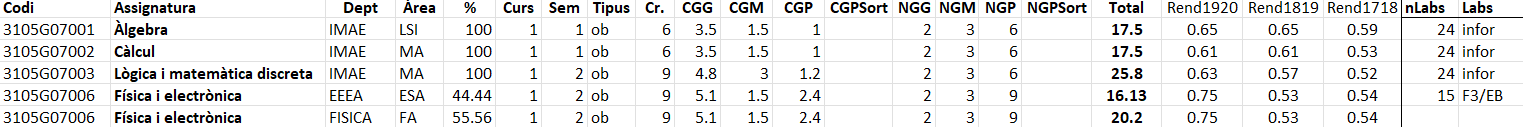
\includegraphics[width=\textwidth]{assets/figs/fitxerPlaDocent.png}
  \caption{\label{img:frag_pla_docent}Fragment del full d'un estudi d'un fitxer de pla docent.}
\end{figure}

\begin{figure}[H]
  \centering
  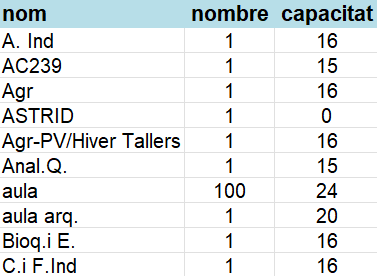
\includegraphics[width=0.4\textwidth]{assets/figs/fitxerPlaDocentLabs.png}
  \caption{\label{img:frag_pla_docent_labs}Fragment del full dels tipus de laboratori d'un fitxer de pla docent.}
\end{figure}

% Citar introducció

\section{Conceptes tècnics}
\label{sec:conceptes_tecnics}

\subsection{Introducció}
\label{subsec:intro_conceptes_tecnics}

En aquesta subsecció, s'introduiran els temes i els conceptes que es tractaran a la resta de la secció.

Tal com s'ha esmentat al capítol~\ref{cap:intro}, la solució informàtica al problema que planteja el projecte s'ha d'implementar en format de plataforma o aplicació web. Si aquest requisit es suma al fet que l'emmagatzematge de dades és totalment necessari, ràpidament es pot concloure que l'arquitectura del sistema és de naturalesa client-servidor i que, consegüentment, es divideix en dues parts diferenciades (veure figura~\ref{img:esquema_web}): l'aplicació client o \textit{front-end} (veure subsecció~\ref{subsec:aplicacio_client}) i l'aplicació servidor o \textit{back-end} (veure subsecció~\ref{subsec:aplicacio_servidor}).

\begin{figure}[H]
  \centering
  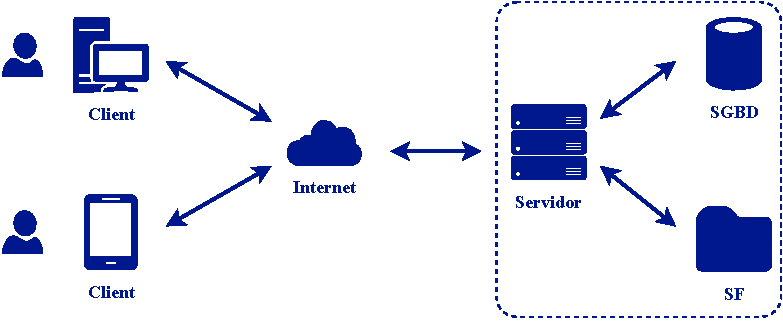
\includegraphics[width=0.95\textwidth]{assets/figs/esquemaWeb.pdf}
  \caption{\label{img:esquema_web}Esquema de l'arquitectura d'una aplicació web convencional.}
\end{figure}

L'aplicació client s'executa sobre un navegador web i s'encarrega principalment d'interactuar amb l'usuari, de manera que pugui visualitzar i manipular les dades emmagatzemades al servidor. Per poder accedir a aquestes dades, l'aplicació client ha de ser capaç de comunicar-se a través d'Internet amb l'aplicació servidor, ja que s'executa a la màquina de l'usuari (veure subsecció~\ref{subsec:comunicacio_cs}).

L'aplicació servidor s'executa fora del navegador en una màquina remota. S'encarrega principalment d'atendre i servir les peticions de consulta o manipulació de dades que rep de les aplicacions client. Davant de cada petició, l'aplicació executa la lògica de negoci corresponent i persisteix les dades necessàries al SF (sistema de fitxers) o a la base de dades, la qual és operada per un SGBD (sistema gestor de bases de dades) (veure subsecció~\ref{subsec:emmagatzematge_dades}). A més a més, a part de simplificar el desenvolupament de l'aplicació client, impedeix l'accés directe a la base de dades des d'Internet, fet que seria molt perillós.

\subsection{Aplicació client}
\label{subsec:aplicacio_client}

En aquesta subsecció, es donaran a conèixer les tecnologies involucrades en el desenvolupament d'aplicacions web client.

Les aplicacions web s'executen sobre un navegador i, generalment, estan compostes pels tres elements bàsics següents:
\begin{itemize}
  \item HTML (\textit{HyperText Markup Language})~\cite{HTML}: Llenguatge de marcat que defineix la semàntica i l'estructura del contingut d'una pàgina web.
  \item CSS (\textit{Cascade Style Sheets})~\cite{CSS}: Llenguatge de fulls d'estil que defineix els estils i la presentació d'un document HTML.
  \item JS (\textit{JavaScript})~\cite{JS}: Llenguatge de programació que defineix la lògica i el comportament del contingut d'una pàgina web i la fa interactiva. Es tracta d'un llenguatge d'un sol fil d'execució, que té suport per a programació orientada a objectes, imperativa i declarativa i que pot ser interpretat o compilat en temps d'execució.
\end{itemize}

Per poder desenvolupar una aplicació web interactiva i dinàmica, en la gran majoria dels casos és necessari treballar amb el DOM mitjançant JavaScript.

El DOM (\textit{Document Object Model}) és una interfície per a documents HTML que n'estructura els elements en forma d'arbre i permet crear-hi, modificar-hi o esborrar-hi nodes, els quals representen un element HTML determinat. A través d'aquesta interfície és possible mutar en temps real el document HTML que el navegador està presentant.

Treballar directament i de manera adequada amb el DOM requereix una comprensió molt profunda del seu funcionament. A mesura que augmenta el dinamisme de l'aplicació i s'implementen interaccions més complexes, el seu desenvolupament es complica notablement i la seva mantenibilitat disminueix. A més a més, requereix una quantitat de temps considerable.

Degut a aquests motius, eventualment van sorgir els \textit{frameworks} JavaScript amb l'objectiu de brindar una millor experiència de desenvolupament i augmentar la mantenibilitat i l'escalabilitat de les aplicacions web.

Un \textit{framework} JavaScript és una infraestructura de \textit{software} que proporciona un conjunt d'eines implementades i provades que serveixen de base per crear aplicacions interactives i escalables. Els \textit{frameworks} abstreuen la gestió del DOM per tal d'estalviar al desenvolupador el fet d'haver de manipular-lo directament en la majoria d'ocasions.

Actualment, existeixen un munt de \textit{frameworks} per escollir. La majoria funcionen de manera similar, però realitzen algunes tasques de manera diferent. Cadascun té els seus avantatges i inconvenients i pot estar enfocat a un tipus d'aplicació concret, cosa que provoca que no n'existeixi un de definitiu. A la pràctica, l'opció més viable sempre depèn del tipus d'aplicació que s'hagi d'implementar. Avui dia, els més populars són React JS, Vue JS, Angular JS i Ember JS, entre d'altres.

Quan es treballa amb aquest tipus de \textit{software} i altres biblioteques de codi, de seguida apareix la necessitat d'unes eines anomenades \textit{bundlers} o ``empaquetadors''.

Abans que els mòduls ES (que permeten la importació i exportació de fragments de codi JavaScript) estéssin disponibles per a navegadors web, els desenvolupadors no tenien cap mecanisme natiu per crear codi JavaScript de manera modular. Per aquest motiu, l'ús de \textit{bundlers} sempre havia sigut necessari per tal de concatenar el codi de \textit{frameworks} i biblioteques en arxius que poguéssin ser executats en el navegador. WebPack, Rollup i Parcel són uns dels \textit{bundlers} més populars.

\subsection{Aplicació servidor}
\label{subsec:aplicacio_servidor}

En aquesta subsecció, es donaran a conèixer les tecnologies involucrades en el desenvolupament d'aplicacions servidor.

A diferència de les aplicacions web client, les aplicacions servidor no estan tan limitades pel que fa a llenguatges de programació. Pràcticament es poden desenvolupar fent servir qualsevol llenguatge. No obstant això, tampoc es lliuren de la necessitat de l'existència de \textit{frameworks} que proporcionin eines que rellevin el desenvolupador en les tasques més comunes, complicades o de baix nivell.

Actualment, hi ha una gran varietat d'opcions a l'hora d'escollir la tecnologia amb la qual s'ha de desenvolupar una determinada aplicació servidor. La tria depèn de múltiples factors, com ara quina és la càrrega de peticions esperada o quina importància té el rendiment envers altres aspectes. Avui dia, els més populars són Firebase, Express.js, Spring Boot, Laravel, Django i Ruby on Rails, entre d'altres.

\subsection{Comunicació entre client i servidor}
\label{subsec:comunicacio_cs}

En aquesta subsecció, es parlarà sobre com s'estableix la comunicació entre l'aplicació client i l'aplicació servidor.

Tal com s'ha pogut veure anteriorment en la secció, l'existència d'eines que permetin implementar la comunicació entre diferents aplicacions és completament essencial. Aquestes eines reben el nom d'API (\textit{application programming interface}) i consisteixen un conjunt de normes i protocols que permeten la comunicació entre dues aplicacions, la qual es realitza mitjançant peticions i respostes.

En el cas de la comunicació entre el \textit{front-end} i el \textit{back-end} d'una aplicació web, es necessiten API enfocades a l'obtenció i manipulació de dades. Al llarg del temps, han sorgit diversos protocols i arquitectures que permeten desenvolupar aquesta tipologia d'API, com ara XML-RPC, SOAP, JSON-RPC, REST o GraphQL.

Actualment, l'opció més popular i utilitzada pel desenvolupament d'aquest tipus d'API és REST (\textit{Representational State Transfer})~\cite{REST}. A diferència d'altres opcions com SOAP, REST no és ni un protocol ni un estàndard, sinó un conjunt de pautes pel que fa a l'arquitectura. Una API és considerada una ``RESTful API'' o ``API REST'' si satisfà tots els principis REST~\cite{REST_CONSTRAINTS}.

Tal com el seu nom indica, quan el client llança una petició contra una API REST, l'API li transfereix una representació de l'estat actual del recurs demanat. La informació s'entrega mitjançant el protocol HTTP (\textit{Hypertext Transfer Protocol})~\cite{HTTP} i en format JSON, XML o HTML, entre d'altres. El format més usat és JSON (\textit{JavaScript Object Notation})~\cite{JSON}, ja que és fàcilment comprensible tant per màquines com persones i, a més, no depèn de cap llenguatge de programació, encara que el seu nom pugui indicar el contrari.

\subsection{Emmagatzematge i gestió de dades}
\label{subsec:emmagatzematge_dades}

En aquesta subsecció, es parlarà sobre com es gestiona l'emmagatzematge de les dades a la banda del servidor.

En els últims anys, les dades s'han convertit en un dels punts més crítics de qualsevol aplicació. La importància d'una bona administració de les dades és clau i beneficiosa tant per a l'usuari del \textit{software} com per a l'organització que l'ha desenvolupat.

No obstant això, aconseguir portar-ho a la pràctica no és tasca senzilla. Aquí és on entren en joc els SGBD (sistemes gestors de bases de dades). Un SGBD és un tipus de programari dedicat a fer d'interfície entre la base de dades i els seus usuaris. Permet administrar, emmagatzemar i recuperar la informació d'una base de dades de manera pràctica, eficient i segura. A més a més, poden implementar funcionalitats addicionals molt útils, com ara visualització de les dades o replicació.

Generalment s'accedeix a les dades mitjançant llenguatges de consulta, com ara SQL (\textit{Structured Query Language}).

Una de les característiques més rellevants dels SGBD és que han de complir sí o sí tots els principis ACID (\textit{Atomicity, Consistency, Isolation, Durability}). Això garantitza la fiabilitat de les seves transaccions, enteses com operacions compostes per d'altres que són individuals. Més concretament, els principis ACID són els següents:
\begin{itemize}
  \item \texttt{Atomicitat:} D'una transacció o se n'executen totes les operacions que la conformen o bé no se n'executa cap.
  \item \texttt{Consistència:} L'estat en el qual es troba la base de dades quan finalitza una transacció ha de ser coherent amb l'estat que tenia abans de que comencés.
  \item \texttt{Aïllament:} Cada transacció s'ha d'executar de manera aïllada envers la resta d'operacions.
  \item \texttt{Definitivitat:} Si es confirma una transacció, el resultat ha de ser definitiu i no es pot perdre.
\end{itemize}

De nou, l'el·lecció d'un SGBD depèn en gran mesura de l'aplicació que s'hagi de desenvolupar. Existeixen un munt d'alternatives enfocades a diferents propòsits: tractament de dades relacionades, gestió de grans volums de dades, consulta molt ràpida, cerques eficients, etc.

Actualment, els SGBD més populars són Oracle, MySQL, PostgreSQL, Redis, Elasticsearch i MongoDB, entre d'altres.


\chapter{Requisits del sistema}
\label{cap:requisits}

\section{Consideracions inicials}
\label{sec:consideracions_inicials}

En aquesta secció, es presentaran una sèrie de consideracions inicials amb l'objectiu de clarificar el contingut de les seccions que segueixen.

En primer lloc, és necessari definir el format que adoptarà cadascun dels requisits del sistema:
\\[8pt]
\centerline{\texttt{\textbf{Tipus-Numeració [Prioritat]}}: Descripció}

Més concretament, el tipus de requisit es representarà mitjançant les seves sigles, com ara \texttt{RF} pels funcionals o \texttt{RNF} pels no funcionals. La numeració es dividirà en grups en funció del rol d'usuari al qual pertanyi el requisit i inclourà la inicial del nom del rol. Pel que fa a la prioritat, se n'han definit tres nivells:
\begin{itemize}
  \item \texttt{Prioritat \textbf{[1]} o essencial:} el compliment total del requisit és de vital importància.
  \item \texttt{Prioritat \textbf{[2]} o moderada:} és important haver desenvolupat, almenys, una part del requisit.
  \item \texttt{Prioritat \textbf{[3]} o addicional:} el compliment del requisit no té gaire rellevància, ja que està més enfocat al treball futur.
\end{itemize}

D'altra banda, cal remarcar que les descripcions dels requisits utilitzen la nomenclatura específica del marc de treball, detallada al capítol~\ref{cap:marcdetreball}.

A més a més, per evitar explicacions redundants, d'ara en endavant, quan es parli de la visualització dels horaris d'un estudi, no s'estarà fent referència a una vista del conglomerat d'horaris de tots els seus cursos i quadrimestres, sinó de vistes en què es mostra l'horari d'un quadrimestre específic en un curs específic. De la mateixa manera, la visualització dels horaris d'un professor o la de l'ocupació d'una aula es separa en quadrimestres.

\section{Requisits funcionals}
\label{sec:requisits_funcionals}

\subsection{Introducció i estructura}
\label{subsec:requisits_funcionals_intro}

En aquesta subsecció, s'introduirà el contingut de la resta de la secció i se'n detallarà l'estructura.

Tal com s'ha pogut veure tant en el capítol~\ref{cap:intro} com en altres, el sistema involucra diversos rols d'usuari. Cada rol ha de poder realitzar un conjunt d'accions determinades i, consegüentment, cadascun comporta una sèrie de requisits diferents.

Per aquest motiu, els requisits funcionals s'han estructurat en funció d'aquests rols: la subsecció~\ref{subsec:requisits_administradors} pels Administradors, la subsecció~\ref{subsec:requisits_coordinadors} pels Coordinadors, la subsecció~\ref{subsec:requisits_director_departament} pels Directors de departament, la subsecció~\ref{subsec:requisits_responsables_docencia} pels Responsables de docència i la subsecció~\ref{subsec:requisits_professors} pels Professors.

A banda d'això, com és natural, també hi ha requisits comuns per a tots els rols, els quals s'agrupen a la subsecció~\ref{subsec:requisits_generals}.

\subsection{Requisits generals}
\label{subsec:requisits_generals}

En aquesta subsecció, es llistaran els requisits funcionals generals del sistema, comuns per a tots els usuaris, independentment dels seus rols.

\begin{itemize}
  \item \texttt{\textbf{RF-G1 [1]}}: Assegurar l'autenticació de tots els usuaris a través d'un formulari de \textit{login}, que s'ha de mostrar a la pantalla quan un usuari no autenticat accedeix a l'aplicació. Sense estar-ho, no l'ha de poder fer servir. L'autenticació d'un usuari ha de suposar la generació d'un \textit{JSON Web Token}~\cite{JWT} (\textit{token} a partir d'ara), per tal de mantenir la seva sessió i poder ser identificat de forma segura pel procés d'autorització de l'aplicació de l'API (o servidor).
  \item \texttt{\textbf{RF-G2 [1]}}: No permetre l'autoregistre d'usuaris, ja que usuaris de determinats rols s'encarregaran de donar d'alta altres usuaris del rol que els correspongui. El procés d'alta d'usuaris es detalla a continuació:
        \begin{enumerate}
          \item L'usuari que registra introdueix les dades de l'usuari que vol donar d'alta, entre les quals consta la seva adreça de correu electrònic. A continuació, l'usuari es crea però amb l'estat de ``desactivat''.
          \item El nou usuari rep un \textit{email} de confirmació amb un enllaç. Mentrestant, no pot autenticar-se a l'aplicació, ja que encara està desactivat.
          \item Un cop l'usuari accedeix a l'enllaç, pot procedir a crear la seva contrasenya mitjançant el formulari presentat a la pantalla. La nova contrasenya s'envia, juntament amb el \textit{token} que conté l'enllaç, al servidor. Si el \textit{token} és vàlid i no ha expirat, l'operació es farà efectiva. La contrasenya s'emmagatzema encriptada.
        \end{enumerate}
  \item \texttt{\textbf{RF-G3 [1]}}: Posar a disposició de l'usuari l'opció de restablir, en cas de pèrdua, la seva contrasenya des de la pàgina de \textit{login}. El procediment ha d'utilitzar el seu correu electrònic com a punt de recuperació i ha de funcionar de manera segura a través d'un \textit{token}.
  \item \texttt{\textbf{RF-G4 [1]}}: L'aplicació del servidor ha d'integrar un mecanisme d'autorització per tal de restringir l'accés als \textit{endpoints} de l'API. Només han de poder utilitzar-los els usuaris que s'hagin autenticat prèviament i que, a més, tinguin permís per fer-ho, de manera que cada \textit{endpoint} sigui accessible només per a un conjunt d'usuaris concret.
  \item \texttt{\textbf{RF-G5 [1]}}: Mostrar en tot moment el nom i el rol de l'usuari autenticat, per tal d'evitar confusions.
  \item \texttt{\textbf{RF-G6 [1]}}: Mostrar un menú que permeti a l'usuari navegar entre les diferents pàgines que exposen les funcionalitats principals corresponents al seu rol.
  \item \texttt{\textbf{RF-G7 [1]}}: Els registres de la base de dades no s'han d'esborrar definitivament. En comptes d'això, tots han de tenir un camp que guardi la data en què han estat eliminats, si és que s'han eliminat. Si no ho estan, aquest camp ha de ser nul.
\end{itemize}


% ADMINISTRADORS
\subsection{Requisits dels Administradors}
\label{subsec:requisits_administradors}

En aquesta subsecció, es llistaran els requisits funcionals particulars dels usuaris amb rol d'Administrador. Cadascun dels apartats que segueixen correspon a una de les seves funcionalitats principals: gestió del pla docent, assignació d'aules, gestió de Coordinadors i gestió de Directors de departament.

\subsubsection{Gestió del pla docent}
\begin{itemize}
  \item \texttt{\textbf{RF-A1 [1]}}: Carregar el pla docent del curs acadèmic següent, de manera que es mantinguin totes les dades que no hagin canviat respecte l'actual.
  \item \texttt{\textbf{RF-A2 [1]}}: Visualitzar les dades del pla docent: estudis i assignatures, departaments i àrees, tipus de laboratori, etc.
  \item \texttt{\textbf{RF-A3 [1]}}: Modificar les dades del pla docent que es llisten a continuació:
  \begin{itemize}
    \item De les assignatures: nombre de grups de cada tipus i àrees i tipus de laboratori assignats.
    \item Dels tipus de laboratori: quantitat d'aules i capacitat d'alumnes.
  \end{itemize}
\end{itemize}

\subsubsection{Assignació d'aules}
\begin{itemize}
  \item \texttt{\textbf{RF-A4 [3]}}: Assignar una aula concreta a cada bloc horari que pugui realitzar-se a més d'una, a mesura que els Coordinadors acabin d'elaborar els horaris que els pertoquin.
\end{itemize}

\subsubsection{Gestió de Coordinadors}
\begin{itemize}
  \item \texttt{\textbf{RF-A5 [1]}}: Visualitzar la llista de les assignacions de Coordinador als diferents estudis.
  \item \texttt{\textbf{RF-A6 [1]}}: Assignar un dels Coordinadors encara no assignats a qualsevol dels estudis.
  \item \texttt{\textbf{RF-A7 [1]}}: Quan es carrega un nou pla docent, s'han de mantenir les assignacions de Coordinador als estudis que ja hi havia a l'anterior.
  \item \texttt{\textbf{RF-A8 [1]}}: Desassignar un Coordinador ja assignat a un estudi.
  \item \texttt{\textbf{RF-A9 [1]}}: Visualitzar el llistat de tots els usuaris Coordinadors, juntament amb la seva informació: nom complet, adreça de correu electrònic, grau al qual està assignat aquest curs acadèmic i si està o no activat.
  \item \texttt{\textbf{RF-A10 [1]}}: Donar d'alta usuaris Coordinadors, és a dir, usuaris amb rol de Coordinador. Per fer-ho, ha d'entrar el seu nom, cognoms i adreça de correu electrònic. A continuació, es duu a terme el procés genèric explicat a la subsecció~\ref{subsec:requisits_generals}. A més a més, ha de poder reenviar-li el correu d'activació.
  \item \texttt{\textbf{RF-A11 [1]}}: Donar de baixa usuaris Coordinadors.
\end{itemize}

\subsubsection{Gestió de Directors de departament}
\begin{itemize}
  \item \texttt{\textbf{RF-A12 [1]}}: Visualitzar la llista de les assignacions de Director de departament als diferents departaments.
  \item \texttt{\textbf{RF-A13 [1]}}: Assignar un dels Directors encara no assignats a qualsevol dels departaments.
  \item \texttt{\textbf{RF-A14 [1]}}: Quan es carrega un nou pla docent, s'han de mantenir les assignacions de Director als departaments que ja hi havia a l'anterior.
  \item \texttt{\textbf{RF-A15 [1]}}: Desassignar un Director ja assignat a un departament.
  \item \texttt{\textbf{RF-A16 [1]}}: Visualitzar el llistat de tots els usuaris Directors de departament, juntament amb la seva informació: nom complet, adreça de correu electrònic, departament al qual està assignat aquest curs acadèmic i si està o no activat.
  \item \texttt{\textbf{RF-A17 [1]}}: Donar d'alta usuaris Directors de departament, és a dir, usuaris amb rol de Director de departament. Per fer-ho, ha d'entrar el seu nom, cognoms i adreça de correu electrònic. A continuació, es duu a terme el procés genèric explicat a la subsecció~\ref{subsec:requisits_generals}. A més a més, ha de poder reenviar-li el correu d'activació.
  \item \texttt{\textbf{RF-A18 [1]}}: Donar de baixa usuaris Directors de departament.
\end{itemize}

% COORDINADORS
\subsection{Requisits dels Coordinadors}
\label{subsec:requisits_coordinadors}

En aquesta subsecció, es llistaran els requisits funcionals particulars dels usuaris amb rol de Coordinador. Cadascun dels apartats que segueixen correspon a una de les seves funcionalitats principals: gestió d'horaris d'estudis, consulta d'horaris de professors i consulta d'horaris d'aules.

\subsubsection{Gestió d'horaris d'estudis}
\begin{itemize}
  \item \texttt{\textbf{RF-C1 [1]}}: Visualitzar els horaris de l'estudi que gestiona, separats en cursos i quadrimestres.
  \item \texttt{\textbf{RF-C2 [1]}}: Visualitzar els horaris dels estudis que ofereixin alguna assignatura compartida amb l'estudi que gestiona.
  \item \texttt{\textbf{RF-C3 [1]}}: Modificar els horaris dels quadrimestres de qualsevol dels cursos de l'estudi que gestiona. El ventall de possibilitats que ha de proporcionar el procés d'edició es detalla a continuació:
  \begin{itemize}
    \item Alternar entre les diferents vistes setmanals, descrites al capítol~\ref{cap:marcdetreball}.
    \item Consultar els blocs horaris pendents de col·locar de manera agrupada per assignatures i tipus de grup.
    \item Consultar la informació completa de qualsevol bloc horari o bloc horari genèric.
    \item Modificar la informació temporal (dia, hora d'inici, duració i setmana) dels blocs horaris i dels blocs horaris genèrics.
    \item Modificar les assignacions a estudis del grup de qualsevol bloc horari l'assignatura del qual sigui compartida.
    \item Modificar l'etiqueta i la subetiqueta dels blocs horaris genèrics.
    \item Oferir la possibilitat d'arrossegar els blocs horaris i els blocs horaris genèrics per tal de modificar-ne la informació temporal.
    \item Oferir la possibilitat d'allargar i escurçar els blocs horaris i els blocs horaris genèrics per tal de modificar-ne l'hora d'inici i la duració.
    \item Crear o esborrar blocs horaris i blocs horaris genèrics.
    \item Aplicar un filtratge de blocs horaris d'assignatures compartides el grup dels quals no estigui assignat a cap estudi.
    \item Aplicar un filtratge de blocs horaris d'assignatures compartides el grup dels quals estigui assignat només a altres estudis.
    \item Quan s'arrossegui un bloc horari, visualitzar una marca sobre les franges en què es produïria algun tipus de solapament en cas que s'hi col·loqués.
    \item Visualitzar una marca sobre els blocs horaris que provoquin solapaments.
    \item Activar o desactivar la visualització de solapaments de cada tipus.
    \item Consultar la informació detallada dels solapaments: veure quins cursos de cada estudi hi estan implicats.
  \end{itemize}
\end{itemize}

\subsubsection{Consulta d'horaris de Professors}
\begin{itemize}
  \item \texttt{\textbf{RF-C4 [2]}}: Visualitzar els horaris dels Professors que imparteixin docència a alguna de les assignatures que ofereixi el grau que gestiona.
\end{itemize}

\subsubsection{Consulta d'horaris d'aules}
\begin{itemize}
  \item \texttt{\textbf{RF-C5 [3]}}: Visualitzar els horaris de l'ocupació de qualsevol aula de l'escola.
\end{itemize}


% DIRECTORS DE DEPARTAMENT
\subsection{Requisits dels Directors de departament}
\label{subsec:requisits_director_departament}

En aquesta subsecció, es llistaran els requisits funcionals particulars dels usuaris amb rol de Director de departament. Cadascun dels apartats que segueixen correspon a una de les seves funcionalitats principals: consulta d'horaris de Professors, consulta d'horaris d'estudis i gestió de Responsables de docència.

\subsubsection{Consulta d'horaris de Professors}
\begin{itemize}
  \item \texttt{\textbf{RF-D1 [3]}}: Visualitzar els horaris dels Professors que imparteixin docència a alguna assignatura de qualsevol de les àrees del seu departament.
\end{itemize}

\subsubsection{Consulta d'horaris d'estudis}
\begin{itemize}
  \item \texttt{\textbf{RF-D2 [2]}}: Visualitzar els horaris dels estudis que ofereixin alguna assignatura de qualsevol de les àrees del seu departament.
\end{itemize}

\subsubsection{Gestió de Responsables de docència}
\begin{itemize}
  \item \texttt{\textbf{RF-D3 [1]}}: Visualitzar la llista de les assignacions de Responsable de docència a les diferents àrees del seu departament.
  \item \texttt{\textbf{RF-D4 [1]}}: Assignar un dels Responsables de docència encara no assignats a qualsevol de les àrees del seu departament.
  \item \texttt{\textbf{RF-D5 [1]}}: Quan es carrega un nou pla docent, s'han de mantenir les assignacions de Responsable de docència a les àrees del seu departament que ja hi havia a l'anterior.
  \item \texttt{\textbf{RF-D6 [1]}}: Desassignar un Responsable de docència ja assignat a una àrea.
  \item \texttt{\textbf{RF-D7 [1]}}: Visualitzar el llistat de tots els usuaris Directors de departament, juntament amb la seva informació: nom complet, adreça de correu electrònic, àrea a la qual està assignat i si està o no activat.
  \item \texttt{\textbf{RF-D8 [1]}}: Donar d'alta usuaris Responsables de docència, és a dir, usuaris amb rol de Responsable de docència. Per fer-ho, ha d'entrar el seu nom, cognoms i adreça de correu electrònic. A continuació, es duu a terme el procés genèric explicat a la subsecció~\ref{subsec:requisits_generals}. A més a més, ha de poder reenviar-li el correu d'activació.
  \item \texttt{\textbf{RF-D9 [1]}}: Donar de baixa usuaris Responsables de docència.
\end{itemize}

% RESPONSABLES DE DOCÈNCIA
\subsection{Requisits dels Responsables de docència}
\label{subsec:requisits_responsables_docencia}

En aquesta subsecció, es llistaran els requisits particulars dels usuaris amb rol de Responsable de docència. Cadascun dels apartats que segueixen correspon a una de les seves funcionalitats principals: consulta d'horaris de Professors, assignació de Professors i gestió de Professors.

\subsubsection{Consulta d'horaris de Professors}
\begin{itemize}
  \item \texttt{\textbf{RF-R1 [3]}}: Visualitzar els horaris dels Professors que imparteixin docència a alguna assignatura de la seva àrea.
\end{itemize}

\subsubsection{Assignació de Professors}
\begin{itemize}
  \item \texttt{\textbf{RF-R2 [2]}}: Assignar un Professor a cada bloc horari de cadascun dels grups de les assignatures de la seva àrea.
  \item \texttt{\textbf{RF-R3 [2]}}: Visualitzar una marca sobre els blocs horaris que provoquin solapaments de Professors.
\end{itemize}

\subsubsection{Gestió de Professors}
\begin{itemize}
  \item \texttt{\textbf{RF-R4 [3]}}: Visualitzar el llistat de tots els usuaris Professors que hagin d'impartir docència a alguna de les assignatures de la seva àrea, juntament amb la seva informació: nom complet, adreça de correu electrònic, assignatures en què imparteix docència i si està o no activat.
  \item \texttt{\textbf{RF-R5 [3]}}: Donar d'alta usuaris Professors, és a dir, usuaris amb rol de Professor. Per fer-ho, ha d'entrar el seu nom, cognoms i adreça de correu electrònic. A continuació, es duu a terme el procés genèric explicat a la subsecció~\ref{subsec:requisits_generals}. A més a més, ha de poder reenviar-li el correu d'activació.
  \item \texttt{\textbf{RF-R6 [3]}}: Donar de baixa usuaris Professors.
\end{itemize}

% PROFESSORS
\subsection{Requisits dels Professors}
\label{subsec:requisits_professors}

En aquesta subsecció, es llistaran els requisits funcionals particulars dels usuaris amb rol de Professor. Cadascun dels apartats que segueixen correspon a una de les seves funcionalitats principals: consulta d'horaris propis, consulta d'horaris d'assignatures, consulta d'horaris d'estudis.

\subsubsection{Consulta d'horaris propis}
\begin{itemize}
  \item \texttt{\textbf{RF-P1 [3]}}: Visualitzar els seus propis horaris, és a dir, els blocs horaris que li han estat assignats.
\end{itemize}

\subsubsection{Consulta d'horaris d'assignatures}
\begin{itemize}
  \item \texttt{\textbf{RF-P2 [3]}}: Visualitzar els horaris de les assignatures a les quals imparteixi docència.
\end{itemize}

\subsubsection{Consulta d'horaris d'estudis}
\begin{itemize}
  \item \texttt{\textbf{RF-P3 [3]}}: Visualitzar els horaris dels estudis que ofereixin alguna de les assignatures en què imparteixi docència.
\end{itemize}

\section{Requisits no funcionals}
\label{sec:requisits_no_funcionals}

En aquesta secció, es llistaran els requisits no funcionals del sistema.

\begin{itemize}
  \item \texttt{\textbf{RNF-1 [1]}}: El client de l'aplicació ha d'executar-se sobre un entorn web i ha de ser suportat pels principals navegadors web. S'ha de poder comunicar amb el procés del servidor mitjançant crides HTTP a l'API del servidor.
  \item \texttt{\textbf{RNF-2 [1]}}: La part de gestió i persistència de dades ha de ser administrada per l'aplicació del servidor, que ha d'exposar una RESTful API. Aquest procés ha de comunicar-se amb els Sistemes Gestors de Bases de Dades escollits per allotjar la informació del projecte.
  \item \texttt{\textbf{RNF-3 [1]}}: Les interfícies d'usuari han d'estar curosament dissenyades i han de ser atractives, intuïtives i, sobretot, eficients.
\end{itemize}

\section{Requisits de domini}
\label{sec:requisits_domini}

En aquesta secció, es llistaran els requisits de domini del sistema.

\begin{itemize}
  \item \texttt{\textbf{RD-1 [1]}}: El format del fitxer que conté les dades del pla docent d'un curs acadèmic està fixat per l'escola (veure capítol~\ref{cap:marcdetreball}).
\end{itemize}

\section{Matriu de dependències}
\label{sec:matriu_dependencies}

En aquesta secció, es representarà la matriu de dependències dels requisits. D'aquesta manera, es podran identificar els requisits funcionals que necessitin l'implementació d'altres per poder-se dur a terme.

El format que adoptarà cadascuna de les dependències es defineix a continuació:
\\[8pt]
\centerline{(\texttt{\textbf{RF-X, RF-Y, \ldots}}) \hspace{1pt} $\longrightarrow$ \hspace{1pt} (\texttt{\textbf{RF-P, RF-Q, \ldots}})}

És a dir, la llista de requisits de la part anterior de la fletxa depèn de la de la part posterior.

La matriu de depedències completa és la següent:

\begin{itemize}
  \item (\texttt{\textbf{RF-G5}}, \texttt{\textbf{RF-G6}}) \hspace{1pt} $\longrightarrow$ \hspace{1pt} (\texttt{\textbf{RF-G1}}, \texttt{\textbf{RF-G2}})
  \item (\texttt{\textbf{RF-A2}}, \texttt{\textbf{RF-A3}}, \texttt{\textbf{RF-A4}}, \texttt{\textbf{RF-A7}}, \texttt{\textbf{RF-A10}}, \texttt{\textbf{RF-A14}}, \texttt{\textbf{RF-A17}}) \hspace{1pt} $\longrightarrow$ \hspace{1pt} (\texttt{\textbf{RF-A1}})
  \item (\texttt{\textbf{RF-C5}}) \hspace{1pt} $\longrightarrow$ \hspace{1pt} (\texttt{\textbf{RF-A4}})
  \item (\texttt{\textbf{RF-A5}}, \texttt{\textbf{RF-A8}}, \texttt{\textbf{RF-C3}}, \texttt{\textbf{RF-C5}}) \hspace{1pt} $\longrightarrow$ \hspace{1pt} (\texttt{\textbf{RF-A6}})
  \item (\texttt{\textbf{RF-A7}}, \texttt{\textbf{RF-A9}}, \texttt{\textbf{RF-A11}}) \hspace{1pt} $\longrightarrow$ \hspace{1pt} (\texttt{\textbf{RF-A10}})
  \item (\texttt{\textbf{RF-A12}}, \texttt{\textbf{RF-A15}}) \hspace{1pt} $\longrightarrow$ \hspace{1pt} (\texttt{\textbf{RF-A13}})
  \item (\texttt{\textbf{RF-A13}}, \texttt{\textbf{RF-A16}}, \texttt{\textbf{RF-A18}}) \hspace{1pt} $\longrightarrow$ \hspace{1pt} (\texttt{\textbf{RF-A17}})
  \item (\texttt{\textbf{RF-A4}, \texttt{\textbf{RF-C1}}, \texttt{\textbf{RF-C2}}, \texttt{\textbf{RF-D2}}, \texttt{\textbf{RF-R1}}, \texttt{\textbf{RF-R2}}}) \hspace{1pt} $\longrightarrow$ \hspace{1pt} (\texttt{\textbf{RF-C3}})
  \item (\texttt{\textbf{RF-D3}}, \texttt{\textbf{RF-D6}}) \hspace{1pt} $\longrightarrow$ \hspace{1pt} (\texttt{\textbf{RF-D4}})
  \item (\texttt{\textbf{RF-D4}}, \texttt{\textbf{RF-D7}}, \texttt{\textbf{RF-D9}}) \hspace{1pt} $\longrightarrow$ \hspace{1pt} (\texttt{\textbf{RF-D8}})
  \item (\texttt{\textbf{RF-C4}}, \texttt{\textbf{RF-D1}}, \texttt{\textbf{RF-R3}}, \texttt{\textbf{RF-P1}}, \texttt{\textbf{RF-P2}}, \texttt{\textbf{RF-P3}}) \hspace{1pt} $\longrightarrow$ \hspace{1pt} (\texttt{\textbf{RF-R2}})
  \item (\texttt{\textbf{RF-R4}}, \texttt{\textbf{RF-R6}}) \hspace{1pt} $\longrightarrow$ \hspace{1pt} (\texttt{\textbf{RF-R5}})
\end{itemize}

\chapter{Planificació}
\label{cap:planificacio}

\section{Descomposició i planificació de tasques}
\label{sec:descomposicio_planificacio_tasques}

\subsection{Estructura i consideracions inicials}
\label{subsec:panificacio_tasques_intro}

En aquesta subsecció es detallarà l'estructura de la resta de la secció i es realitzaran una sèrie de consideracions inicials amb l'objectiu de clarificar-ne el contingut.

Tal com s'ha vist al capítol~\ref{cap:metodologia}, la gestió del projecte es basa en el PMBOK. Més concretament, en la metodologia de desenvolupament WBS, a través de la qual es durà a terme una descomposició del projecte en paquets de treball per tal d'organitzar i planificar totes les tasques que s'hi involucren.

Primerament, es definirà un esquema arbòric que representi les diferents parts que conformen el projecte des d'una visió generalista. Cadascuna d'aquestes parts conformarà una subsecció.

Tot seguit, s'aprofundirà en cadascuna de les branques d'aquest arbre general i es determinaran els diversos paquets de treball que les formen. Degut a la grandària d'alguna de les branques, és possible que en alguns casos siguin necessàries més descomposicions.

Cada paquet de treball contindrà la informació següent:
\begin{itemize}
  \item \textbf{Identificador}: Codi que servirà per referir-se al paquet en seccions posteriors.
  \item \textbf{Nom}: Nom que se li haurà donat al paquet als esquemes arbòrics.
  \item \textbf{Descripció}: Descripció breu del paquet.
  \item \textbf{Tasques}: Conjunt de tasques que s'han de realitzar en el paquet.
  \item \textbf{Temporalització}: Estimació del temps que es necessitarà per completar les tasques del paquet.
  \item \textbf{Lliurable}: Resultat palpable que s'obtindrà un cop completades les tasques del paquet.
\end{itemize}

És molt important destacar que la planificació s'ha fet tenint en compte el 100\% del projecte, sense les acotacions marcades al capítol~\ref{cap:intro}. Gràcies a això, es pot observar que sense aquestes acotacions la data de finalització estimada del projecte se'n va massa enllà (veure secció~\ref{sec:temporalitzacio}).

\subsection{Visió general}
\label{subsec:visio_general}

En aquesta subsecció, es mostrarà la descomposició general de les tasques del projecte en branques, tal com es pot veure a la figura~\ref{img:pt_general}.

\begin{figure}[H]
	\centering
	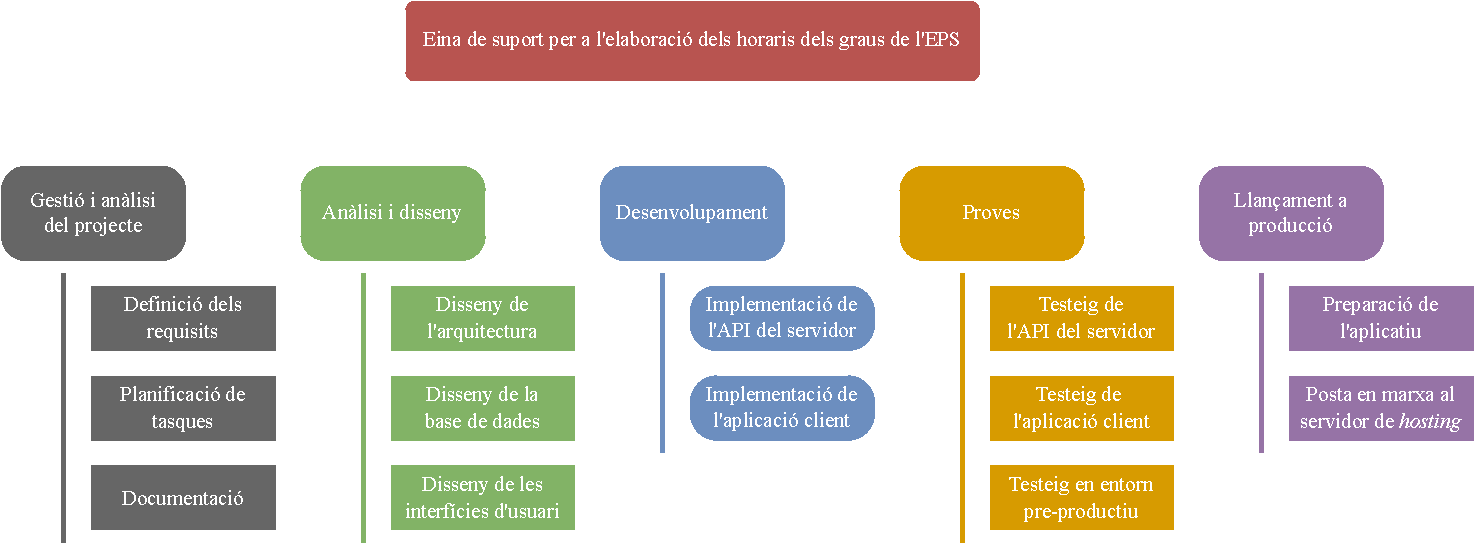
\includegraphics[width=\textwidth]{assets/working_packages/general.pdf}
	\caption{\label{img:pt_general}Descomposició general de les tasques del projecte.}
\end{figure}

\newpage

\subsection{Gestió del projecte}
\label{subsec:gestio_projecte}

En aquesta subsecció, s'exposaran els paquets de treball que formen part de la branca de planificació \emph{Gestió del projecte}.

Tal com es pot veure a la figura~\ref{img:pt_gestio_projecte}, els paquets de treball de la gesió del projecte són la definició dels requisits, la planificació de tasques i la documentació (veure taules~\ref{taula:pt_1.1},~\ref{taula:pt_1.2} i~\ref{taula:pt_1.3}, respectivament).

\begin{figure}[H]
	\centering
	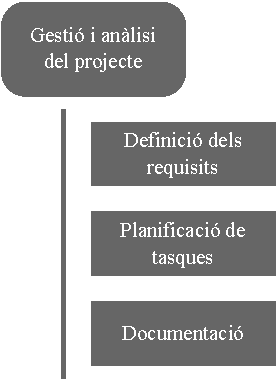
\includegraphics[width=0.35\textwidth]{assets/working_packages/gestioProjecte.pdf}
	\caption{\label{img:pt_gestio_projecte}Esquema de la branca de planificació \emph{Gestió del projecte}.}
\end{figure}

\begin{table}[H]
  \begin{tabularx}{\textwidth}{l | X}
    \toprule
    \rowcolor{Gray}
    \multicolumn{2}{c}{\texttt{\textbf{PT\_1.1:}} Definició dels requisits}\\
    \midrule[0.9pt]
    \textbf{Descripció}       & Anàlisi dels requisits que ha de complir l'aplicatiu del projecte.\\
    \midrule
    \textbf{Tasques}          & \textbf{T1:} Anàlisi i definició dels requisits no funcionals.
    \newline \textbf{T2:} Anàlisi i definició dels requisits de domini.
    \newline \textbf{T3:} Anàlisi i definició dels requisits funcionals.
    \newline \textbf{T4:} Confecció de la matriu de dependències entre els requisits.
    \newline \textbf{T5:} Verificació i comentari dels requisits amb els tutors.
    \newline \textbf{T6:} Correcció del document de requisits.\\
    \midrule
    \textbf{Temporalització}  & 45 hores.\\
    \midrule
    \textbf{Lliurable}        & Document de requisits del sistema (veure capítol~\ref{cap:requisits}).\\
    \bottomrule
  \end{tabularx}
  \caption{\label{taula:pt_1.1} Taula del paquet de treball \emph{Definició dels requisits}.}
\end{table}

\begin{table}[H]
  \begin{tabularx}{\textwidth}{l | X}
    \toprule
    \rowcolor{Gray}
    \multicolumn{2}{c}{\texttt{\textbf{PT\_1.2:}} Planificació de tasques}\\
    \midrule[0.9pt]
    \textbf{Descripció}       & Planificació de totes les tasques que involucra el projecte.\\
    \midrule
    \textbf{Tasques}          & \textbf{T1:} Descomposició i agrupació general de les tasques.
    \newline \textbf{T2:} Determinació i elaboració dels paquets de treball de cada grup de tasques.
    \newline \textbf{T3:} Confecció de la matriu de traçabilitat.
    \newline \textbf{T4:} Estimació del temps necessari per al desenvolupament del projecte i elaboració del cronograma.\\
    \midrule
    \textbf{Temporalització}  & 30 hores.\\
    \midrule
    \textbf{Lliurable}        & Documents de planificació i temporalització del projecte (veure capítol~\ref{cap:planificacio}).\\
    \bottomrule
  \end{tabularx}
  \caption{\label{taula:pt_1.2} Taula del paquet de treball \emph{Planificació de tasques}.}
\end{table}

\begin{table}[H]
  \begin{tabularx}{\textwidth}{l | X}
    \toprule
    \rowcolor{Gray}
    \multicolumn{2}{c}{\texttt{\textbf{PT\_1.3:}} Documentació}\\
    \midrule[0.9pt]
    \textbf{Descripció}       & Confecció del document de la memòria del projecte.\\
    \midrule
    \textbf{Tasques}          & \textbf{T1:} Redacció de la memòria del projecte.
    \newline \textbf{T2:} Verificació i comentari de la memòria amb els tutors.
    \newline \textbf{T3:} Correcció i retocament final de la memòria.\\
    \midrule
    \textbf{Temporalització}  & 200 hores.\\
    \midrule
    \textbf{Lliurable}        & Memòria del projecte.\\
    \bottomrule
  \end{tabularx}
  \caption{\label{taula:pt_1.3} Taula del paquet de treball \emph{Documentació}.}
\end{table}

\newpage

\subsection{Anàlisi i disseny}
\label{subsec:analisi_disseny}

En aquesta subsecció, s'exposaran els paquets de treball que formen part de la branca de planificació \emph{Anàlisi i disseny}.

Tal com es pot veure a la figura~\ref{img:pt_analisi_disseny}, els paquets de treball de l'anàlisi i disseny són: el disseny de l'arquitectura, el disseny de la base de dades i el disseny de les interfícies d'usuari (veure taules~\ref{taula:pt_2.1},~\ref{taula:pt_2.2} i~\ref{taula:pt_2.3}, respectivament).

\begin{figure}[htpb]
	\centering
	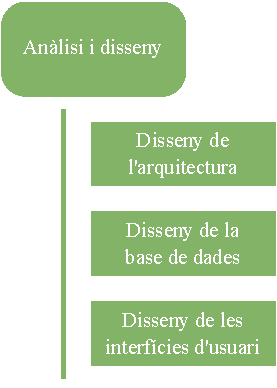
\includegraphics[width=0.35\textwidth]{assets/working_packages/analisiDisseny.pdf}
	\caption{\label{img:pt_analisi_disseny}Esquema de la branca de planificació \emph{Anàlisi i disseny}.}
\end{figure}

\begin{table}[H]
  \begin{tabularx}{\textwidth}{l | X}
    \toprule
    \rowcolor{Green}
    \multicolumn{2}{c}{\texttt{\textbf{PT\_2.1:}} Disseny de l'arquitectura}\\
    \midrule[0.9pt]
    \textbf{Descripció}       & Estudi i disseny de l'arquitectura de l'aplicatiu del projecte.\\
    \midrule
    \textbf{Tasques}          & \textbf{T1:} Estudi dels requisits.
    \newline \textbf{T2:} Estudi i decisió del tipus de base de dades que s'utilitzarà i del seu sistema gestor.
    \newline \textbf{T3:} Estudi i decisió del tipus de tecnologia amb la qual s'implementarà l'aplicació web client.
    \newline \textbf{T4:} Estudi i decisió del tipus de tecnologia amb la qual s'implementarà l'aplicació servidor.\\
    \midrule
    \textbf{Temporalització}  & 15 hores.\\
    \midrule
    \textbf{Lliurable}        & Document de valoració i justificació de les tecnologies que conformen l'arquitectura de l'aplicatiu del projecte.\\
    \bottomrule
  \end{tabularx}
  \caption{\label{taula:pt_2.1} Taula del paquet de treball \emph{Disseny de l'arquitectura}.}
\end{table}

\begin{table}[H]
  \begin{tabularx}{\textwidth}{l | X}
    \toprule
    \rowcolor{Green}
    \multicolumn{2}{c}{\texttt{\textbf{PT\_2.2:}} Disseny de la base de dades}\\
    \midrule[0.9pt]
    \textbf{Descripció}       & Disseny de l'estructura de la base de dades de l'aplicatiu i determinació de la informació que s'hi emmagatzemarà.\\
    \midrule
    \textbf{Tasques}          & \textbf{T1:} Detall de les entitats que conformaran la base de dades.
    \newline \textbf{T2:} Decisió dels camps en què es dividiran les entitats, juntament amb el seu tipus i configuració.
    \newline \textbf{T3:} Determinació de les relacions que existiran entre les diferents entitats.
    \newline \textbf{T4:} Elaboració de l'esquema del model relacional.\\
    \midrule
    \textbf{Temporalització}  & 25 hores.\\
    \midrule
    \textbf{Lliurable}        & Esquema del model relacional de la base de dades.\\
    \bottomrule
  \end{tabularx}
  \caption{\label{taula:pt_2.2} Taula del paquet de treball \emph{Disseny de la base de dades}.}
\end{table}

\begin{table}[H]
  \begin{tabularx}{\textwidth}{l | X}
    \toprule
    \rowcolor{Green}
    \multicolumn{2}{c}{\texttt{\textbf{PT\_2.3:}} Disseny de les interfícies d'usuari}\\
    \midrule[0.9pt]
    \textbf{Descripció}       & Disseny de les interfícies d'usuari que es presentaran a l'aplicació web client.\\
    \midrule
    \textbf{Tasques}          & \textbf{T1:} Confecció dels esquemes de les interfícies d'usuari de les diferents parts de l'aplicació.
    \newline \textbf{T2:} Anàlisi dels esquemes i verificació de la seva adaptació als requisits.
    \newline \textbf{T3:} Plantejament de possibles nous requisits que hagin pogut sorgir a partir dels esquemes.\\
    \midrule
    \textbf{Temporalització}  & 85 hores.\\
    \midrule
    \textbf{Lliurable}        & Esquemes de les interfícies d'usuari de l'aplicació web client.\\
    \bottomrule
  \end{tabularx}
  \caption{\label{taula:pt_2.3} Taula del paquet de treball \emph{Disseny de les interfícies d'usuari}.}
\end{table}

\newpage

\subsection{Desenvolupament}
\label{subsec:desenvolupament}

En aquesta subsecció, s'exposaran els paquets de treball que formen part de la branca de planificació \emph{Desenvolupament} (veure figura~\ref{img:pt_desenvolupament}).

A diferència de la resta de branques, aquesta no conté directament un conjunt de paquets de treball, sinó que en deriven altres branques. Als apartats següents es detallaran els paquets de treball que conté cadascuna.

\begin{figure}[H]
	\centering
	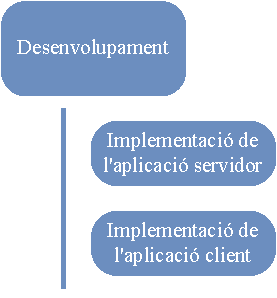
\includegraphics[width=0.35\textwidth]{assets/working_packages/desenvolupament/general.pdf}
	\caption{\label{img:pt_desenvolupament}Esquema de la branca de planificació \emph{Desenvolupament}.}
\end{figure}

\newpage

\subsubsection{Implementació de l'aplicació servidor}
\label{subsubsec:implementacio_api}

Tal com es pot veure a la figura~\ref{img:pt_implementacio_api}, els paquets de treball de la implementació de l'aplicació servidor són: la preparació inicial, la configuració de la base de dades, la definició dels models de dades, la implementació de l'enrutament, la implementació del \textit{login} i del registre i la implementació dels serveis (veure taules~\ref{taula:pt_3.1.1},~\ref{taula:pt_3.1.2},~\ref{taula:pt_3.1.3},~\ref{taula:pt_3.1.4},~\ref{taula:pt_3.1.5} i~\ref{taula:pt_3.1.6}, respectivament).

\begin{figure}[H]
	\centering
	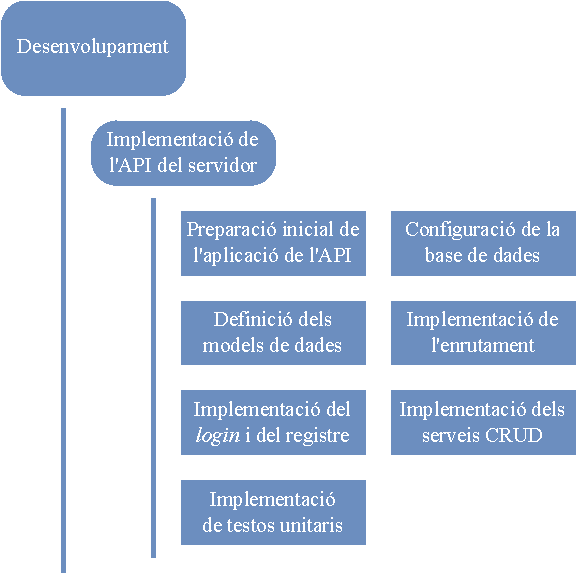
\includegraphics[width=0.7\textwidth]{assets/working_packages/desenvolupament/implementacioAPI.pdf}
	\caption{\label{img:pt_implementacio_api}Esquema de la branca de planificació derivada \emph{Implementació de l'aplicació servidor}.}
\end{figure}

\newpage

\begin{table}[H]
  \begin{tabularx}{\textwidth}{l | X}
    \toprule
    \rowcolor{Blue}
    \multicolumn{2}{c}{\texttt{\textbf{PT\_3.1.1:}} Preparació inicial}\\
    \midrule[0.9pt]
    \textbf{Descripció}       & Preparació i configuració inicial de l'aplicació servidor.\\
    \midrule
    \textbf{Tasques}          & \textbf{T1:} Preparació de l'entorn de desenvolupament.
    \newline \textbf{T2:} Configuració del procés d'escolta de peticions.
    \newline \textbf{T3:} Implementació del tractament general de peticions i d'errors.
    \newline \textbf{T4:} Implementació del sistema de depuració i monitoreig.
    \newline \textbf{T5:} Implementació del sistema de configuració i variables d'entorn.\\
    \midrule
    \textbf{Temporalització}  & 25 hores.\\
    \midrule
    \textbf{Lliurable}        & Aplicació servidor preparada per ser implementada.\\
    \bottomrule
  \end{tabularx}
  \caption{\label{taula:pt_3.1.1} Taula del paquet de treball \emph{Preparació inicial de l'aplicació servidor}.}
\end{table}

\begin{table}[H]
  \begin{tabularx}{\textwidth}{l | X}
    \toprule
    \rowcolor{Blue}
    \multicolumn{2}{c}{\texttt{\textbf{PT\_3.1.2:}} Configuració de la base de dades}\\
    \midrule[0.9pt]
    \textbf{Descripció}       & Configuració inicial del sistema gestor de la base de dades i de l'ORM (\textit{object relational mapper}).\\
    \midrule
    \textbf{Tasques}          & \textbf{T1:} Configuració de la connexió entre l'aplicació de l'API i el sistema gestor de la base de dades.
    \newline \textbf{T2:} Configuració de l'ORM escollit.
    \newline \textbf{T3:} Determinació dels usuaris del sistema gestor de la base de dades.\\
    \midrule
    \textbf{Temporalització}  & 5 hores.\\
    \midrule
    \textbf{Lliurable}        & Sistema gestor de la base de dades configurat.\\
    \bottomrule
  \end{tabularx}
  \caption{\label{taula:pt_3.1.2} Taula del paquet de treball \emph{Configuració de la base de dades}.}
\end{table}

\newpage

\begin{table}[H]
  \begin{tabularx}{\textwidth}{l | X}
    \toprule
    \rowcolor{Blue}
    \multicolumn{2}{c}{\texttt{\textbf{PT\_3.1.3:}} Definició dels models de dades}\\
    \midrule[0.9pt]
    \textbf{Descripció}       & Definició dels models de dades que s'han de guardar a la base de dades.\\
    \midrule
    \textbf{Tasques}          & \textbf{T1:} Definició i configuració dels models de dades descrits a l'esquema del model relacional.
    \newline \textbf{T2:} Implementació de validadors de dades per a cada camp dels models.
    \newline \textbf{T3:} Implementació i configuració de les relacions entre models.\\
    \midrule
    \textbf{Temporalització}  & 30 hores.\\
    \midrule
    \textbf{Lliurable}        & Models de dades definits.\\
    \bottomrule
  \end{tabularx}
  \caption{\label{taula:pt_3.1.3} Taula del paquet de treball \emph{Definició dels models de dades}.}
\end{table}

\begin{table}[H]
  \begin{tabularx}{\textwidth}{l | X}
    \toprule
    \rowcolor{Blue}
    \multicolumn{2}{c}{\texttt{\textbf{PT\_3.1.4:}} Implementació de l'enrutament}\\
    \midrule[0.9pt]
    \textbf{Descripció}       & Definició dels diferents \textit{endpoints} de l'API i implementació de l'enrutament de peticions.\\
    \midrule
    \textbf{Tasques}          & \textbf{T1:} Definició dels \textit{endpoints} de l'API i de les seves rutes.
    \newline \textbf{T2:} Implementació de l'enrutament de peticions a l'\textit{endpoint} corresponent.
    \newline \textbf{T3:} Implementació dels mecanismes d'autorització segons el rol de l'usuari.\\
    \midrule
    \textbf{Temporalització}  & 20 hores.\\
    \midrule
    \textbf{Lliurable}        & Enrutament implementat.\\
    \bottomrule
  \end{tabularx}
  \caption{\label{taula:pt_3.1.4} Taula del paquet de treball \emph{Implementació de l'enrutament}.}
\end{table}

\newpage

\begin{table}[H]
  \begin{tabularx}{\textwidth}{l | X}
    \toprule
    \rowcolor{Blue}
    \multicolumn{2}{c}{\texttt{\textbf{PT\_3.1.5:}} Implementació del \textit{login} i del registre}\\
    \midrule[0.9pt]
    \textbf{Descripció}       & Implementació del tractament de peticions d'autenticació i de registre d'usuaris.\\
    \midrule
    \textbf{Tasques}          & \textbf{T1:} Implementació inicial dels processos d'autenticació i de registre.
    \newline \textbf{T2:} Implementació dels mecanismes de seguretat involucrats.
    \newline \textbf{T3:} Implementació de l'enviament dels correus electrònics involucrats.\\
    \midrule
    \textbf{Temporalització}  & 30 hores.\\
    \midrule
    \textbf{Lliurable}        & \textit{Login} i registre implementats.\\
    \bottomrule
  \end{tabularx}
  \caption{\label{taula:pt_3.1.5} Taula del paquet de treball \emph{Implementació del \textit{login} i del registre}.}
\end{table}

\begin{table}[H]
  \begin{tabularx}{\textwidth}{l | X}
    \toprule
    \rowcolor{Blue}
    \multicolumn{2}{c}{\texttt{\textbf{PT\_3.1.6:}} Implementació dels serveis CRUD.}\\
    \midrule[0.9pt]
    \textbf{Descripció}       & Implementació dels serveis de creació, recuperació, modificació i eliminació per a cadascun dels models de dades.\\
    \midrule
    \textbf{Tasques}          & \textbf{T1:} Implementació dels serveis CRUD per als models de dades relacionats amb els Administradors.
    \newline \textbf{T2:} Implementació dels serveis CRUD per als models de dades relacionats amb els Coordinadors.
    \newline \textbf{T3:} Implementació dels serveis CRUD per als models de dades relacionats amb els Directors de departament.
    \newline \textbf{T4:} Implementació dels serveis CRUD per als models de dades relacionats amb els Responsables de docència.
    \newline \textbf{T5:} Implementació dels serveis CRUD per als models de dades relacionats amb els Professors.\\
    \midrule
    \textbf{Temporalització}  & 85 hores.\\
    \midrule
    \textbf{Lliurable}        & Serveis de CRUD implementats.\\
    \bottomrule
  \end{tabularx}
  \caption{\label{taula:pt_3.1.6} Taula del paquet de treball \emph{Implementació dels serveis CRUD.}}
\end{table}

\newpage

\subsubsection{Implementació de l'aplicació client}
\label{subsubsec:implementacio_client}

Tal com es pot veure a la figura~\ref{img:pt_implementacio_client}, els paquets de treball de l'implementació de l'aplicació client són: la preparació inicial de l'aplicació client, la implementació del \textit{login} i relacionats, la implementació de la part dels Administradors, la implementació de la part dels Coordinadors, la implementació de la part dels Directors de departament, la implementació de la part dels Responsables de docència i la implementació de la part dels Professors (veure taules~\ref{taula:pt_3.2.1},~\ref{taula:pt_3.2.2},~\ref{taula:pt_3.2.3},~\ref{taula:pt_3.2.4},~\ref{taula:pt_3.2.5},~\ref{taula:pt_3.2.6} i~\ref{taula:pt_3.2.7}, respectivament).

\begin{figure}[H]
	\centering
	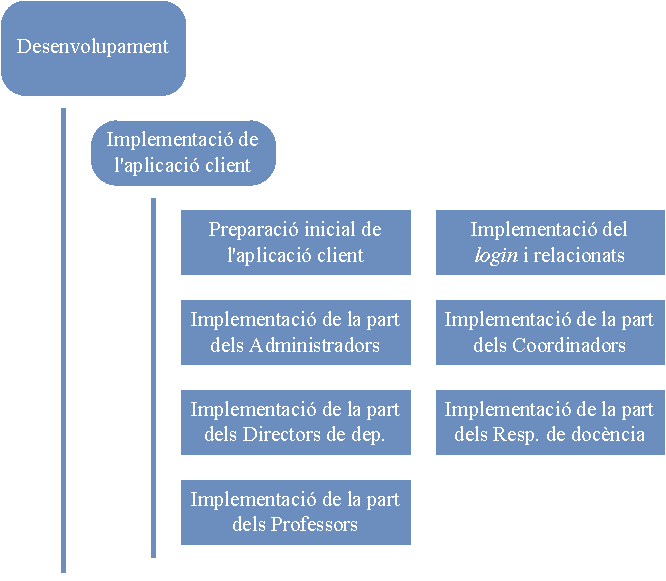
\includegraphics[width=0.7\textwidth]{assets/working_packages/desenvolupament/implementacioClient.pdf}
	\caption{\label{img:pt_implementacio_client}Esquema de la branca de planificació derivada \emph{Implementació del client}.}
\end{figure}

\begin{table}[H]
  \begin{tabularx}{\textwidth}{l | X}
    \toprule
    \rowcolor{Blue}
    \multicolumn{2}{c}{\texttt{\textbf{PT\_3.2.1:}} Preparació inicial de l'aplicació client}\\
    \midrule[0.9pt]
    \textbf{Descripció}       & Preparació i configuració inicials de l'aplicació client.\\
    \midrule
    \textbf{Tasques}          & \textbf{T1:} Preparació de l'entorn de desenvolupament.\\
    \midrule
    \textbf{Temporalització}  & 10 hores.\\
    \midrule
    \textbf{Lliurable}        & Aplicació client preparada per ser implementada.\\
    \bottomrule
  \end{tabularx}
  \caption{\label{taula:pt_3.2.1} Taula del paquet de treball \emph{Preparació inicial de l'aplicació client}.}
\end{table}

\begin{table}[H]
  \begin{tabularx}{\textwidth}{l | X}
    \toprule
    \rowcolor{Blue}
    \multicolumn{2}{c}{\texttt{\textbf{PT\_3.2.2:}} Implementació del \textit{login} i relacionats}\\
    \midrule[0.9pt]
    \textbf{Descripció}       & Implementació de les finestres i procediments relacionats amb l'autenticació dels usuaris.\\
    \midrule
    \textbf{Tasques}          & \textbf{T1:} Implementació de la finestra d'autenticació.
    \newline \textbf{T2:} Implementació del conjunt de finestres de restabliment de contrasenya.\\
    \midrule
    \textbf{Temporalització}  & 40 hores.\\
    \midrule
    \textbf{Lliurable}        & Finestres i procediments de \textit{login} i relacionats implementats.\\
    \bottomrule
  \end{tabularx}
  \caption{\label{taula:pt_3.2.2} Taula del paquet de treball \emph{Implementació del \textit{login} i relacionats}.}
\end{table}

\begin{table}[H]
  \begin{tabularx}{\textwidth}{l | X}
    \toprule
    \rowcolor{Blue}
    \multicolumn{2}{c}{\texttt{\textbf{PT\_3.2.3:}} Implementació de la part dels Administradors}\\
    \midrule[0.9pt]
    \textbf{Descripció}       & Implementació de les finestres i procediments que involucren els usuaris amb rol d'Administrador.\\
    \midrule
    \textbf{Tasques}          & \textbf{T1:} Implementació del conjunt de finestres relacionades amb la gestió de plans docents.
    \newline \textbf{T2:} Implementació del conjunt de finestres relacionades amb l'assignació d'aules.
    \newline \textbf{T3:} Implementació del conjunt de finestres relacionades amb la gestió de Coordinadors.
    \newline \textbf{T4:} Implementació del conjunt de finestres relacionades amb la gestió de Directors de departament.\\
    \midrule
    \textbf{Temporalització}  & 80 hores.\\
    \midrule
    \textbf{Lliurable}        & Part dels usuaris Administradors implementada.\\
    \bottomrule
  \end{tabularx}
  \caption{\label{taula:pt_3.2.3} Taula del paquet de treball \emph{Implementació de la part dels Administradors}.}
\end{table}

\newpage

\begin{table}[H]
  \begin{tabularx}{\textwidth}{l | X}
    \toprule
    \rowcolor{Blue}
    \multicolumn{2}{c}{\texttt{\textbf{PT\_3.2.4:}} Implementació de la part dels Coordinadors}\\
    \midrule[0.9pt]
    \textbf{Descripció}       & Implementació de les finestres i procediments que involucren els usuaris amb rol de Coordinador.\\
    \midrule
    \textbf{Tasques}          & \textbf{T1:} Implementació del conjunt de finestres relacionades amb la gestió d'horaris d'estudis.
    \newline \textbf{T2:} Implementació del conjunt de finestres relacionades amb la consulta d'horaris de Professors.
    \newline \textbf{T3:} Implementació del conjunt de finestres relacionades amb la consulta d'horaris d'aules.\\
    \midrule
    \textbf{Temporalització}  & 150 hores.\\
    \midrule
    \textbf{Lliurable}        & Part dels usuaris Coordinadors implementada.\\
    \bottomrule
  \end{tabularx}
  \caption{\label{taula:pt_3.2.4} Taula del paquet de treball \emph{Implementació de la part dels Coordinadors}.}
\end{table}

\begin{table}[H]
  \begin{tabularx}{\textwidth}{l | X}
    \toprule
    \rowcolor{Blue}
    \multicolumn{2}{c}{\texttt{\textbf{PT\_3.2.5:}} Implementació de la part dels Directors de departament}\\
    \midrule[0.9pt]
    \textbf{Descripció}       & Implementació de les finestres i procediments que involucren els usuaris amb rol de Director de departament.\\
    \midrule
    \textbf{Tasques}          & \textbf{T1:} Implementació del conjunt de finestres relacionades amb la consulta d'horaris de Professors.
    \newline \textbf{T2:} Implementació del conjunt de finestres relacionades amb la consulta d'horaris d'estudis.
    \newline \textbf{T3:} Implementació del conjunt de finestres relacionades amb la gestió de Responsables de docència.\\
    \midrule
    \textbf{Temporalització}  & 15 hores.\\
    \midrule
    \textbf{Lliurable}        & Part dels usuaris Directors de departament implementada.\\
    \bottomrule
  \end{tabularx}
  \caption{\label{taula:pt_3.2.5} Taula del paquet de treball \emph{Implementació de la part dels Directors de departament}.}
\end{table}

\newpage

\begin{table}[H]
  \begin{tabularx}{\textwidth}{l | X}
    \toprule
    \rowcolor{Blue}
    \multicolumn{2}{c}{\texttt{\textbf{PT\_3.2.6:}} Implementació de la part dels Responsables de docència}\\
    \midrule[0.9pt]
    \textbf{Descripció}       & Implementació de les finestres i procediments que involucren els usuaris amb rol de Responsable de docència.\\
    \midrule
    \textbf{Tasques}          & \textbf{T1:} Implementació del conjunt de finestres relacionades amb la consulta d'horaris de Professors.
    \newline \textbf{T2:} Implementació del conjunt de finestres relacionades amb l'assignació de Professors.
    \newline \textbf{T3:} Implementació del conjunt de finestres relacionades amb la gestió de Professors.\\
    \midrule
    \textbf{Temporalització}  & 40 hores.\\
    \midrule
    \textbf{Lliurable}        & Part dels usuaris Responsables de docència implementada.\\
    \bottomrule
  \end{tabularx}
  \caption{\label{taula:pt_3.2.6} Taula del paquet de treball \emph{Implementació de la part dels Responsables de docència}.}
\end{table}

\begin{table}[H]
  \begin{tabularx}{\textwidth}{l | X}
    \toprule
    \rowcolor{Blue}
    \multicolumn{2}{c}{\texttt{\textbf{PT\_3.2.7:}} Implementació de la part dels Professors}\\
    \midrule[0.9pt]
    \textbf{Descripció}       & Implementació de les finestres i procediments que involucren els usuaris amb rol de Professor.\\
    \midrule
    \textbf{Tasques}          & \textbf{T1:} Implementació del conjunt de finestres relacionades amb la consulta dels propis horaris.
    \newline \textbf{T2:} Implementació del conjunt de finestres relacionades amb la consulta d'horaris d'assignatures.
    \newline \textbf{T3:} Implementació del conjunt de finestres relacionades amb la consulta d'horaris de'estudis.\\
    \midrule
    \textbf{Temporalització}  & 15 hores.\\
    \midrule
    \textbf{Lliurable}        & Part dels usuaris Professors implementada.\\
    \bottomrule
  \end{tabularx}
  \caption{\label{taula:pt_3.2.7} Taula del paquet de treball \emph{Implementació de la part dels Professors}.}
\end{table}

\newpage

\subsection{Proves}
\label{subsec:proves}

En aquesta subsecció, s'exposaran els paquets de treball que formen part de la branca de planificació \emph{Proves}.

Tal com es pot veure a la figura~\ref{img:pt_proves}, els paquets de treball de les proves són el testeig de l'aplicació servidor, el testeig de l'aplicació client i el testeig general de casos d'ús (veure taules~\ref{taula:pt_4.1},~\ref{taula:pt_4.2} i~\ref{taula:pt_4.3}, respectivament).

Cal destacar que el testeig tant de l'aplicació client com de l'aplicació servidor no està previst efectuar-se només al final de tota la fase de desenvolupament, sinó que s'anirà fent de manera progressiva a mesura que avança la implementació.

\begin{figure}[htpb]
	\centering
	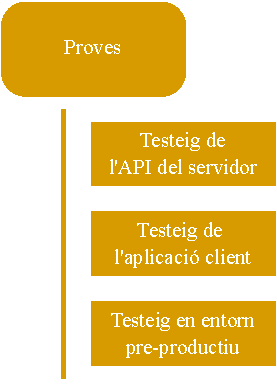
\includegraphics[width=0.35\textwidth]{assets/working_packages/proves.pdf}
	\caption{\label{img:pt_proves}Esquema de la branca de planificació \emph{Proves}.}
\end{figure}

\begin{table}[H]
  \begin{tabularx}{\textwidth}{l | X}
    \toprule
    \rowcolor{Orange}
    \multicolumn{2}{c}{\texttt{\textbf{PT\_4.1:}} Testeig de l'aplicació servidor}\\
    \midrule[0.9pt]
    \textbf{Descripció}       & Realització de proves manuals i depuració de l'aplicació servidor.\\
    \midrule
    \textbf{Tasques}          & \textbf{T1:} Disseny de les proves que s'han de realitzar.
    \newline \textbf{T2:} Efectuació de les proves i anàlisi dels resultats.
    \newline \textbf{T3:} Correcció dels errors que hagin pogut aparèixer.\\
    \midrule
    \textbf{Temporalització}  & 40 hores.\\
    \midrule
    \textbf{Lliurable}        & Proves i depuració de l'aplicació servidor realitzades.\\
    \bottomrule
  \end{tabularx}
  \caption{\label{taula:pt_4.1} Taula del paquet de treball \emph{Testeig de l'aplicació servidor}.}
\end{table}

\begin{table}[H]
  \begin{tabularx}{\textwidth}{l | X}
    \toprule
    \rowcolor{Orange}
    \multicolumn{2}{c}{\texttt{\textbf{PT\_4.2:}} Testeig de l'aplicació client}\\
    \midrule[0.9pt]
    \textbf{Descripció}       & Realització de proves manuals i depuració de l'aplicació client.\\
    \midrule
    \textbf{Tasques}          & \textbf{T1:} Disseny de les proves que s'han de realitzar.
    \newline \textbf{T2:} Efectuació de les proves i anàlisi dels resultats.
    \newline \textbf{T3:} Correcció dels errors que hagin pogut aparèixer.\\
    \midrule
    \textbf{Temporalització}  & 50 hores.\\
    \midrule
    \textbf{Lliurable}        & Proves i depuració de l'aplicació client realitzada.\\
    \bottomrule
  \end{tabularx}
  \caption{\label{taula:pt_4.2} Taula del paquet de treball \emph{Testeig de l'aplicació client}.}
\end{table}

\begin{table}[H]
  \begin{tabularx}{\textwidth}{l | X}
    \toprule
    \rowcolor{Orange}
    \multicolumn{2}{c}{\texttt{\textbf{PT\_4.3:}} Testeig general de casos d'ús}\\
    \midrule[0.9pt]
    \textbf{Descripció}       & Realització de proves i depuració replicant manualment casos d'ús reals.\\
    \midrule
    \textbf{Tasques}          & \textbf{T1:} Simulació de situacions reals a mode de prova.
    \newline \textbf{T2:} Correcció dels errors que hagin pogut aparèixer.\\
    \midrule
    \textbf{Temporalització}  & 20 hores.\\
    \midrule
    \textbf{Lliurable}        & Proves i depuració en un entorn pre-productiu realitzada.\\
    \bottomrule
  \end{tabularx}
  \caption{\label{taula:pt_4.3} Taula del paquet de treball \emph{Testeig general de casos d'ús}.}
\end{table}

\subsection{Llançament a producció}
\label{subsec:llancament_produccio}

En aquesta subsecció, s'exposaran els paquets de treball que formen part de la branca de planificació \emph{Llançament a producció}.

Tal com es pot veure a la figura~\ref{img:pt_llancament_roduccio}, els paquets de treball del llançament a producció són la preparació de l'aplicatiu i la posada en marxa al servidor de \textit{hosting} (veure taules~\ref{taula:pt_5.1} i~\ref{taula:pt_5.2}, respectivament).

Cal destacar que la posada en marxa en l'entorn productiu no forma part l'abast del projecte i que, per tant, no es comptabilitzarà en el còmput de temps total. Tot i així, per tal d'obtenir una planificació completa, s'ha decidit contemplar-ho.

\begin{figure}[htpb]
	\centering
	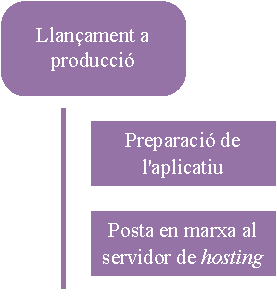
\includegraphics[width=0.35\textwidth]{assets/working_packages/llancamentProduccio.pdf}
	\caption{\label{img:pt_llancament_roduccio}Esquema de la branca de planificació \emph{Llançament a producció}.}
\end{figure}

\begin{table}[H]
  \begin{tabularx}{\textwidth}{l | X}
    \toprule
    \rowcolor{Purple}
    \multicolumn{2}{c}{\texttt{\textbf{PT\_5.1:}} Preparació de l'aplicatiu}\\
    \midrule[0.9pt]
    \textbf{Descripció}       & Preparació de l'aplicatiu per al llançament a producció.\\
    \midrule
    \textbf{Tasques}          & \textbf{T1:} Revisió i neteja del codi font.
    \newline \textbf{T2:} Verificació que no es mostra cap informació en pantalla o en consola que pugui comprometre la seguretat.
    \newline \textbf{T3:} Comprovació que les variables d'entorn es recuperen correctament.
    \newline \textbf{T4:} Verificar els arxius de configuració.\\
    \midrule
    \textbf{Temporalització}  & 10 hores.\\
    \midrule
    \textbf{Lliurable}        & Aplicatiu preparat per al llançament a producció.\\
    \bottomrule
  \end{tabularx}
  \caption{\label{taula:pt_5.1} Taula del paquet de treball \emph{Preparació de l'aplicatiu}.}
\end{table}

\begin{table}[H]
  \begin{tabularx}{\textwidth}{l | X}
    \toprule
    \rowcolor{Purple}
    \multicolumn{2}{c}{\texttt{\textbf{PT\_5.2:}} Posada en marxa al servidor de \textit{hosting}}\\
    \midrule[0.9pt]
    \textbf{Descripció}       & Llançament a producció de l'aplicatiu al servidor de \textit{hosting}.\\
    \midrule
    \textbf{Tasques}          & \textbf{T1:} Configuració general del servidor.
    \newline \textbf{T2:} Traspàs de l'aplicatiu al servidor.
    \newline \textbf{T3:} Establiment de les variables d'entorn corresponents.
    \newline \textbf{T4:} Posada en marxa de l'aplicatiu i realització de comprovacions.\\
    \midrule
    \textbf{Temporalització}  & 25 hores.\\
    \midrule
    \textbf{Lliurable}        & Aplicatiu en funcionament a l'entorn productiu.\\
    \bottomrule
  \end{tabularx}
  \caption{\label{taula:pt_5.2} Taula del paquet de treball \emph{Posada en marxa al servidor de \textit{hosting}}.}
\end{table}


\section{Matriu de traçabilitat}
\label{sec:matriu_tracabilitat}

En aquesta secció, es representarà la matriu de traçabilitat que relaciona els paquets de treball definits a la secció~\ref{sec:descomposicio_planificacio_tasques} i els requisits definits al capítol~\ref{cap:requisits}.

D'aquesta manera, es podrà saber quins requisits s'assoleixen un cop completades les tasques dels paquets de treball.

El format que adoptarà cadascuna de les relacions es defineix a continuació:
\\[8pt]
\centerline{(\texttt{\textbf{RF-X}, \texttt{\textbf{RF-Y}}}, \texttt{\textbf{\ldots}}) $\longrightarrow$ (\texttt{\textbf{PT\_P}}, \texttt{\textbf{PT\_Q}, \texttt{\textbf{\ldots}}})}

És a dir, la llista de requisits de la part anterior de la flexta s'assoleix un cop completada la de paquets de treball situada a la part posterior.

La matriu de traçabilitat completa és la següent:
\begin{itemize}
  \item (\texttt{\textbf{RF-G1}}, \texttt{\textbf{RF-G3}}) \hspace{1pt} $\longrightarrow$ \hspace{1pt} (\texttt{\textbf{PT\_3.1.5}}, \texttt{\textbf{PT\_3.2.2}})
  \item (\texttt{\textbf{RF-G2}}) \hspace{1pt} $\longrightarrow$ \hspace{1pt} (\texttt{\textbf{PT\_3.1.5}}, \texttt{\textbf{PT\_3.2.3}}, \texttt{\textbf{PT\_3.2.5}}, \texttt{\textbf{PT\_3.2.6}})
  \item (\texttt{\textbf{RF-G5}}, \texttt{\textbf{RF-G6}}) \hspace{1pt} $\longrightarrow$ \hspace{1pt} (\texttt{\textbf{PT\_3.1.6}}, \texttt{\textbf{PT\_3.2.3}}, \texttt{\textbf{PT\_3.2.4}}, \texttt{\textbf{PT\_3.2.5}},\\
  \texttt{\textbf{PT\_3.2.6}}, \texttt{\textbf{PT\_3.2.7}})
  \item (\texttt{\textbf{RF-G4}}) \hspace{1pt} $\longrightarrow$ \hspace{1pt} (\texttt{\textbf{PT\_3.1.4}})
  \item (\texttt{\textbf{RF-G7}}) \hspace{1pt} $\longrightarrow$ \hspace{1pt} (\texttt{\textbf{PT\_2.2}}, \texttt{\textbf{PT\_3.1.2}}, \texttt{\textbf{PT\_3.1.3}})
  \item (\texttt{\textbf{RF-A1}}, \texttt{\textbf{RF-A2}}, \texttt{\textbf{RF-A3}}, \texttt{\textbf{RF-A4}}, \texttt{\textbf{RF-A5}}, \texttt{\textbf{RF-A6}}, \texttt{\textbf{RF-A7}}, \texttt{\textbf{RF-A8}}, \texttt{\textbf{RF-A9}}, \texttt{\textbf{RF-A11}}, \texttt{\textbf{RF-A12}}, \texttt{\textbf{RF-A13}}, \texttt{\textbf{RF-A14}}, \texttt{\textbf{RF-A15}}, \texttt{\textbf{RF-A16}}, \texttt{\textbf{RF-A18}}) \hspace{1pt} $\longrightarrow$ \hspace{1pt} (\texttt{\textbf{PT\_3.1.6}},\\
  \texttt{\textbf{PT\_3.2.3}})
  \item (\texttt{\textbf{RF-A10}}, \texttt{\textbf{RF-A17}}) \hspace{1pt} $\longrightarrow$ \hspace{1pt} (\texttt{\textbf{PT\_3.1.5}}, \texttt{\textbf{PT\_3.1.6}}, \texttt{\textbf{PT\_3.2.3}})
  \item (\texttt{\textbf{RF-C1}}, \texttt{\textbf{RF-C2}}, \texttt{\textbf{RF-C3}}, \texttt{\textbf{RF-C4}}, \texttt{\textbf{RF-C5}}) \hspace{1pt} $\longrightarrow$ \hspace{1pt} (\texttt{\textbf{PT\_3.1.6}}, \texttt{\textbf{PT\_3.2.4}})
  \item (\texttt{\textbf{RF-D1}}, \texttt{\textbf{RF-D2}}, \texttt{\textbf{RF-D3}}, \texttt{\textbf{RF-D4}}, \texttt{\textbf{RF-D5}}, \texttt{\textbf{RF-D6}}, \texttt{\textbf{RF-D7}}, \texttt{\textbf{RF-D9}}) \hspace{1pt} $\longrightarrow$ \hspace{1pt} (\texttt{\textbf{PT\_3.1.6}},\\
  \texttt{\textbf{PT\_3.2.5}})
  \item (\texttt{\textbf{RF-D8}}) \hspace{1pt} $\longrightarrow$ \hspace{1pt} (\texttt{\textbf{PT\_3.1.5}}, \texttt{\textbf{PT\_3.1.6}}, \texttt{\textbf{PT\_3.2.5}})
  \item (\texttt{\textbf{RF-R1}}, \texttt{\textbf{RF-R2}}, \texttt{\textbf{RF-R3}}, \texttt{\textbf{RF-R4}}, \texttt{\textbf{RF-R6}}) \hspace{1pt} $\longrightarrow$ \hspace{1pt} (\texttt{\textbf{PT\_3.1.6}}, \texttt{\textbf{PT\_3.2.6}})
  \item (\texttt{\textbf{RF-R5}}, \texttt{\textbf{RF-G3}}) \hspace{1pt} $\longrightarrow$ \hspace{1pt} (\texttt{\textbf{PT\_3.1.5}}, \texttt{\textbf{PT\_3.1.6}}, \texttt{\textbf{PT\_3.2.6}})
  \item (\texttt{\textbf{RF-P1}}, \texttt{\textbf{RF-P2}}, \texttt{\textbf{RF-P3}}) \hspace{1pt} $\longrightarrow$ \hspace{1pt} (\texttt{\textbf{PT\_3.1.6}}, \texttt{\textbf{PT\_3.2.7}})
\end{itemize}

\section{Temporalització}
\label{sec:temporalitzacio}

\subsection{Determinació d'activitats}
\label{subsec:determinacio_activitats}

En aquesta subsecció, a partir de la matriu de dependències (veure secció~\ref{sec:matriu_dependencies}) i la de traçabilitat (veure secció~\ref{sec:matriu_tracabilitat}), es determinaran les activitats que caldrà dur a terme per completar el desenvolupament del projecte.

Una activitat és una agrupació de paquets de treball i/o de tasques de paquets de treball que cal completar per poder assolir una sèrie de requisits.

Un cop s'hagin determinat les activitats, s'efectuarà una estimació del temps que podria requerir completar cadascuna. Aquesta estimació consistirà, primerament, en indicar tres valors de temps:

\begin{itemize}
  \item \textit{t(O)}: Estimació optimista.
  \item \textit{t(M)}: El més probable.
  \item \textit{t(P)}: Estimació pessimista.
\end{itemize}

Tot seguit, es calcularà el temps esperat de duració \textit{t(E)} de l'activitat. Aquest càlcul consisteix en una mitjana ponderada dels valors de l'estimació anterior, tal com es pot veure a continuació:

\begin{equation*}
  t(E) = \frac{t(O) + 4t(M) + t(P)}{6}
\end{equation*}

Les taules marcades en gris (\ref{taula:a1},~\ref{taula:a2} i~\ref{taula:a21}) corresponen a la fase de gestió del projecte, les marcades en verd (\ref{taula:a3},~\ref{taula:a4} i~\ref{taula:a5}) a la d'anàlisi i disseny, les marcades en blau (\ref{taula:a6},~\ref{taula:a7},~\ref{taula:a8},~\ref{taula:a9},~\ref{taula:a10},~\ref{taula:a11},~\ref{taula:a12},~\ref{taula:a13},~\ref{taula:a14},~\ref{taula:a15} i~\ref{taula:a16}) a la de desenvolupament, les marcades en taronja (\ref{taula:a17},~\ref{taula:a18} i~\ref{taula:a19}) a la de proves i, finalment, la marcada en lila (\ref{taula:a20}) a la de llançament a producció

\begin{table}[H]
  \begin{tabularx}{\textwidth}{l | X}
    \toprule
    \rowcolor{Gray}
    \multicolumn{2}{c}{\texttt{\textbf{A1:}} Definició de requisits}\\
    \midrule[0.9pt]
    \textbf{Tasques}                 & \texttt{\textbf{PT\_1.1}}.\\
    \midrule
    \textbf{Estimació de temps}      & \textit{t(O)}: 30 hores.
    \newline \textit{t(M)}: 45 hores.
    \newline \textit{t(P)}: 60 hores.\\
    \midrule
    \textbf{Durada esperada}         & \textbf{\textit{t(E)}: 45 hores}.\\
    \bottomrule
  \end{tabularx}
  \caption{\label{taula:a1} Taula de l'activitat \emph{Definició de requisits}.}
\end{table}

\begin{table}[H]
  \begin{tabularx}{\textwidth}{l | X}
    \toprule
    \rowcolor{Gray}
    \multicolumn{2}{c}{\texttt{\textbf{A2:}} Planificació de tasques}\\
    \midrule[0.9pt]
    \textbf{Tasques}                 & \texttt{\textbf{PT\_1.2}}.\\
    \midrule
    \textbf{Estimació de temps}      & \textit{t(O)}: 25 hores.
    \newline \textit{t(M)}: 30 hores.
    \newline \textit{t(P)}: 50 hores.\\
    \midrule
    \textbf{Durada esperada}         & \textbf{\textit{t(E)}: 33 hores}.\\
    \bottomrule
  \end{tabularx}
  \caption{\label{taula:a2} Taula de l'activitat \emph{Planificació de tasques}.}
\end{table}

\begin{table}[H]
  \begin{tabularx}{\textwidth}{l | X}
    \toprule
    \rowcolor{Green}
    \multicolumn{2}{c}{\texttt{\textbf{A3:}} Disseny de l'arquitectura}\\
    \midrule[0.9pt]
    \textbf{Tasques}                 & \texttt{\textbf{PT\_2.1}}.\\
    \midrule
    \textbf{Estimació de temps}      & \textit{t(O)}: 10 hores.
    \newline \textit{t(M)}: 15 hores.
    \newline \textit{t(P)}: 30 hores.\\
    \midrule
    \textbf{Durada esperada}         & \textbf{\textit{t(E)}: 17 hores}.\\
    \bottomrule
  \end{tabularx}
  \caption{\label{taula:a3} Taula de l'activitat \emph{Disseny de l'arquitectura}.}
\end{table}

\begin{table}[H]
  \begin{tabularx}{\textwidth}{l | X}
    \toprule
    \rowcolor{Green}
    \multicolumn{2}{c}{\texttt{\textbf{A4:}} Disseny de la base de dades}\\
    \midrule[0.9pt]
    \textbf{Tasques}                 & \texttt{\textbf{PT\_2.2}}.\\
    \midrule
    \textbf{Estimació de temps}      & \textit{t(O)}: 15 hores.
    \newline \textit{t(M)}: 25 hores.
    \newline \textit{t(P)}: 30 hores.\\
    \midrule
    \textbf{Durada esperada}         & \textbf{\textit{t(E)}: 24 hores}.\\
    \bottomrule
  \end{tabularx}
  \caption{\label{taula:a4} Taula de l'activitat \emph{Disseny de la base de dades}.}
\end{table}

\begin{table}[H]
  \begin{tabularx}{\textwidth}{l | X}
    \toprule
    \rowcolor{Green}
    \multicolumn{2}{c}{\texttt{\textbf{A5:}} Disseny de les interfícies d'usuari}\\
    \midrule[0.9pt]
    \textbf{Tasques}                 & \texttt{\textbf{PT\_2.3}}.\\
    \midrule
    \textbf{Estimació de temps}      & \textit{t(O)}: 60 hores.
    \newline \textit{t(M)}: 85 hores.
    \newline \textit{t(P)}: 120 hores.\\
    \midrule
    \textbf{Durada esperada}         & \textbf{\textit{t(E)}: 87 hores}.\\
    \bottomrule
  \end{tabularx}
  \caption{\label{taula:a5} Taula de l'activitat \emph{Disseny de les interfícies d'usuari}.}
\end{table}

\begin{table}[H]
  \begin{tabularx}{\textwidth}{l | X}
    \toprule
    \rowcolor{Blue}
    \multicolumn{2}{c}{\texttt{\textbf{A6:}} Preparació inicial de l'aplicació servidor}\\
    \midrule[0.9pt]
    \textbf{Tasques}                 & \texttt{\textbf{PT\_3.1.1}}.\\
    \midrule
    \textbf{Estimació de temps}      & \textit{t(O)}: 20 hores.
    \newline \textit{t(M)}: 25 hores.
    \newline \textit{t(P)}: 30 hores.\\
    \midrule
    \textbf{Durada esperada}         & \textbf{\textit{t(E)}: 25 hores}.\\
    \bottomrule
  \end{tabularx}
  \caption{\label{taula:a6} Taula de l'activitat \emph{Preparació inicial de l'aplicació servidor}.}
\end{table}

\begin{table}[H]
  \begin{tabularx}{\textwidth}{l | X}
    \toprule
    \rowcolor{Blue}
    \multicolumn{2}{c}{\texttt{\textbf{A7:}} Configuració de la base de dades}\\
    \midrule[0.9pt]
    \textbf{Tasques}                 & \texttt{\textbf{PT\_3.1.2}}.\\
    \midrule
    \textbf{Estimació de temps}      & \textit{t(O)}: 4 hores.
    \newline \textit{t(M)}: 5 hores.
    \newline \textit{t(P)}: 20 hores.\\
    \midrule
    \textbf{Durada esperada}         & \textbf{\textit{t(E)}: 8 hores}.\\
    \bottomrule
  \end{tabularx}
  \caption{\label{taula:a7} Taula de l'activitat \emph{Configuració de la base de dades}.}
\end{table}

\begin{table}[H]
  \begin{tabularx}{\textwidth}{l | X}
    \toprule
    \rowcolor{Blue}
    \multicolumn{2}{c}{\texttt{\textbf{A8:}} Definició dels models de dades}\\
    \midrule[0.9pt]
    \textbf{Tasques}                 & \texttt{\textbf{PT\_3.1.3}}.\\
    \midrule
    \textbf{Estimació de temps}      & \textit{t(O)}: 25 hores.
    \newline \textit{t(M)}: 30 hores.
    \newline \textit{t(P)}: 35 hores.\\
    \midrule
    \textbf{Durada esperada}         & \textbf{\textit{t(E)}: 30 hores}.\\
    \bottomrule
  \end{tabularx}
  \caption{\label{taula:a8} Taula de l'activitat \emph{Definició dels models de dades}.}
\end{table}

\begin{table}[H]
  \begin{tabularx}{\textwidth}{l | X}
    \toprule
    \rowcolor{Blue}
    \multicolumn{2}{c}{\texttt{\textbf{A9:}} Implementació de l'enrutament}\\
    \midrule[0.9pt]
    \textbf{Tasques}                 & \texttt{\textbf{PT\_3.1.4}}.\\
    \midrule
    \textbf{Estimació de temps}      & \textit{t(O)}: 15 hores.
    \newline \textit{t(M)}: 20 hores.
    \newline \textit{t(P)}: 25 hores.\\
    \midrule
    \textbf{Durada esperada}         & \textbf{\textit{t(E)}: 25 hores}.\\
    \bottomrule
  \end{tabularx}
  \caption{\label{taula:a9} Taula de l'activitat \emph{Implementació de l'enrutament}.}
\end{table}

\begin{table}[H]
  \begin{tabularx}{\textwidth}{l | X}
    \toprule
    \rowcolor{Blue}
    \multicolumn{2}{c}{\texttt{\textbf{A10:}} Preparació inicial de l'aplicació client}\\
    \midrule[0.9pt]
    \textbf{Tasques}                 & \texttt{\textbf{PT\_3.2.1}}.\\
    \midrule
    \textbf{Estimació de temps}      & \textit{t(O)}: 8 hores.
    \newline \textit{t(M)}: 10 hores.
    \newline \textit{t(P)}: 15 hores.\\
    \midrule
    \textbf{Durada esperada}         & \textbf{\textit{t(E)}: 11 hores}.\\
    \bottomrule
  \end{tabularx}
  \caption{\label{taula:a10} Taula de l'activitat \emph{Preparació inicial de l'aplicació client}.}
\end{table}

\begin{table}[H]
  \begin{tabularx}{\textwidth}{l | X}
    \toprule
    \rowcolor{Blue}
    \multicolumn{2}{c}{\texttt{\textbf{A11:}} Implementació del \textit{login} i relacionats}\\
    \midrule[0.9pt]
    \textbf{Tasques}                 & \texttt{\textbf{PT\_3.1.5}}, \texttt{\textbf{PT\_3.2.2}}.\\
    \midrule
    \textbf{Estimació de temps}      & \textit{t(O)}: 55 hores.
    \newline \textit{t(M)}: 70 hores.
    \newline \textit{t(P)}: 80 hores.\\
    \midrule
    \textbf{Durada esperada}         & \textbf{\textit{t(E)}: 69 hores}.\\
    \bottomrule
  \end{tabularx}
  \caption{\label{taula:a11} Taula de l'activitat \emph{Implementació del \textit{login} i relacionats}.}
\end{table}

\begin{table}[H]
  \begin{tabularx}{\textwidth}{l | X}
    \toprule
    \rowcolor{Blue}
    \multicolumn{2}{c}{\texttt{\textbf{A12:}} Implementació de la part dels Administradors}\\
    \midrule[0.9pt]
    \textbf{Tasques}                 & [\textbf{T1}] de \texttt{\textbf{PT\_3.1.6}}, \texttt{\textbf{PT\_3.2.3}}.\\
    \midrule
    \textbf{Estimació de temps}      & \textit{t(O)}: 90 hores.
    \newline \textit{t(M)}: 95 hores.
    \newline \textit{t(P)}: 110 hores.\\
    \midrule
    \textbf{Durada esperada}         & \textbf{\textit{t(E)}: 97 hores}.\\
    \bottomrule
  \end{tabularx}
  \caption{\label{taula:a12} Taula de l'activitat \emph{Implementació de la part dels Administradors}.}
\end{table}

\begin{table}[H]
  \begin{tabularx}{\textwidth}{l | X}
    \toprule
    \rowcolor{Blue}
    \multicolumn{2}{c}{\texttt{\textbf{A13:}} Implementació de la part dels Coordinadors}\\
    \midrule[0.9pt]
    \textbf{Tasques}                 & [\textbf{T2}] de \texttt{\textbf{PT\_3.1.6}}, \texttt{\textbf{PT\_3.2.4}}.\\
    \midrule
    \textbf{Estimació de temps}      & \textit{t(O)}: 140 hores.
    \newline \textit{t(M)}: 165 hores.
    \newline \textit{t(P)}: 180 hores.\\
    \midrule
    \textbf{Durada esperada}         & \textbf{\textit{t(E)}: 164 hores}.\\
    \bottomrule
  \end{tabularx}
  \caption{\label{taula:a13} Taula de l'activitat \emph{Implementació de la part dels Coordinadors}.}
\end{table}

\begin{table}[H]
  \begin{tabularx}{\textwidth}{l | X}
    \toprule
    \rowcolor{Blue}
    \multicolumn{2}{c}{\texttt{\textbf{A14:}} Implementació de la part dels Directors de departament}\\
    \midrule[0.9pt]
    \textbf{Tasques}                 & [\textbf{T3}] de \texttt{\textbf{PT\_3.1.6}}, \texttt{\textbf{PT\_3.2.5}}.\\
    \midrule
    \textbf{Estimació de temps}      & \textit{t(O)}: 20 hores.
    \newline \textit{t(M)}: 30 hores.
    \newline \textit{t(P)}: 40 hores.\\
    \midrule
    \textbf{Durada esperada}         & \textbf{\textit{t(E)}: 30 hores}.\\
    \bottomrule
  \end{tabularx}
  \caption{\label{taula:a14} Taula de l'activitat \emph{Implementació de la part dels Directors de departament}.}
\end{table}

\begin{table}[H]
  \begin{tabularx}{\textwidth}{l | X}
    \toprule
    \rowcolor{Blue}
    \multicolumn{2}{c}{\texttt{\textbf{A15:}} Implementació de la part dels Responsables de docència}\\
    \midrule[0.9pt]
    \textbf{Tasques}                 & [\textbf{T4}] de \texttt{\textbf{PT\_3.1.6}}, \texttt{\textbf{PT\_3.2.6}}.\\
    \midrule
    \textbf{Estimació de temps}      & \textit{t(O)}: 50 hores.
    \newline \textit{t(M)}: 55 hores.
    \newline \textit{t(P)}: 70 hores.\\
    \midrule
    \textbf{Durada esperada}         & \textbf{\textit{t(E)}: 57 hores}.\\
    \bottomrule
  \end{tabularx}
  \caption{\label{taula:a15} Taula de l'activitat \emph{Implementació de la part dels Responsables de docència}.}
\end{table}

\begin{table}[H]
  \begin{tabularx}{\textwidth}{l | X}
    \toprule
    \rowcolor{Blue}
    \multicolumn{2}{c}{\texttt{\textbf{A16:}} Implementació de la part dels Professors}\\
    \midrule[0.9pt]
    \textbf{Tasques}                 & [\textbf{T5}] de \texttt{\textbf{PT\_3.1.6}}, \texttt{\textbf{PT\_3.2.7}}.\\
    \midrule
    \textbf{Estimació de temps}      & \textit{t(O)}: 10 hores.
    \newline \textit{t(M)}: 30 hores.
    \newline \textit{t(P)}: 40 hores.\\
    \midrule
    \textbf{Durada esperada}         & \textbf{\textit{t(E)}: 30 hores}.\\
    \bottomrule
  \end{tabularx}
  \caption{\label{taula:a16} Taula de l'activitat \emph{Implementació de la part dels Professors}.}
\end{table}

\begin{table}[H]
  \begin{tabularx}{\textwidth}{l | X}
    \toprule
    \rowcolor{Orange}
    \multicolumn{2}{c}{\texttt{\textbf{A17:}} Testeig de l'aplicació servidor}\\
    \midrule[0.9pt]
    \textbf{Tasques}                 & \texttt{\textbf{PT\_4.1}}.\\
    \midrule
    \textbf{Estimació de temps}      & \textit{t(O)}: 20 hores.
    \newline \textit{t(M)}: 40 hores.
    \newline \textit{t(P)}: 50 hores.\\
    \midrule
    \textbf{Durada esperada}         & \textbf{\textit{t(E)}: 39 hores}.\\
    \bottomrule
  \end{tabularx}
  \caption{\label{taula:a17} Taula de l'activitat \emph{Testeig de l'aplicació servidor}.}
\end{table}

\begin{table}[H]
  \begin{tabularx}{\textwidth}{l | X}
    \toprule
    \rowcolor{Orange}
    \multicolumn{2}{c}{\texttt{\textbf{A18:}} Testeig de l'aplicació client}\\
    \midrule[0.9pt]
    \textbf{Tasques}                 & \texttt{\textbf{PT\_4.2}}.\\
    \midrule
    \textbf{Estimació de temps}      & \textit{t(O)}: 30 hores.
    \newline \textit{t(M)}: 50 hores.
    \newline \textit{t(P)}: 60 hores.\\
    \midrule
    \textbf{Durada esperada}         & \textbf{\textit{t(E)}: 49 hores}.\\
    \bottomrule
  \end{tabularx}
  \caption{\label{taula:a18} Taula de l'activitat \emph{Testeig de l'aplicació client}.}
\end{table}

\begin{table}[H]
  \begin{tabularx}{\textwidth}{l | X}
    \toprule
    \rowcolor{Orange}
    \multicolumn{2}{c}{\texttt{\textbf{A19:}} Testeig general de casos d'ús}\\
    \midrule[0.9pt]
    \textbf{Tasques}                 & \texttt{\textbf{PT\_4.3}}.\\
    \midrule
    \textbf{Estimació de temps}      & \textit{t(O)}: 10 hores.
    \newline \textit{t(M)}: 20 hores.
    \newline \textit{t(P)}: 30 hores.\\
    \midrule
    \textbf{Durada esperada}         & \textbf{\textit{t(E)}: 20 hores}.\\
    \bottomrule
  \end{tabularx}
  \caption{\label{taula:a19} Taula de l'activitat \emph{Testeig general de casos d'ús}.}
\end{table}

\begin{table}[H]
  \begin{tabularx}{\textwidth}{l | X}
    \toprule
    \rowcolor{Purple}
    \multicolumn{2}{c}{\texttt{\textbf{A20:}} Posada en marxa de l'aplicatiu}\\
    \midrule[0.9pt]
    \textbf{Tasques}                 & \texttt{\textbf{PT\_5.1}}, \texttt{\textbf{PT\_5.2}}.\\
    \midrule
    \textbf{Estimació de temps}      & \textit{t(O)}: 25 hores.
    \newline \textit{t(M)}: 35 hores.
    \newline \textit{t(P)}: 50 hores.\\
    \midrule
    \textbf{Durada esperada}         & \textbf{\textit{t(E)}: 36 hores}.\\
    \bottomrule
  \end{tabularx}
  \caption{\label{taula:a20} Taula de l'activitat \emph{Posada en marxa de l'aplicatiu}.}
\end{table}

\begin{table}[H]
  \begin{tabularx}{\textwidth}{l | X}
    \toprule
    \rowcolor{Gray}
    \multicolumn{2}{c}{\texttt{\textbf{A21:}} Documentació}\\
    \midrule[0.9pt]
    \textbf{Tasques}                 & \texttt{\textbf{PT\_1.3}}.\\
    \midrule
    \textbf{Estimació de temps}      & \textit{t(O)}: 150 hores.
    \newline \textit{t(M)}: 200 hores.
    \newline \textit{t(P)}: 220 hores.\\
    \midrule
    \textbf{Durada esperada}         & \textbf{\textit{t(E)}: 195 hores}.\\
    \bottomrule
  \end{tabularx}
  \caption{\label{taula:a21} Taula de l'activitat \emph{Documentació}.}
\end{table}

\newpage

\subsection{Diagrama d'activitats}
\label{subsec:diagrama_activitats}

En aquesta subsecció, s'il·lustrarà el diagrama de les activitats planificades a la subsecció~\ref{subsec:determinacio_activitats}.

Tal com es pot veure a la figura~\ref{img:diagrama_activitats}, el diagrama consistirà en un graf els vèrtexs del qual representen activitats i les arestes relacions ``acabar per començar''. Les arestes també duran el temps esperat de durada de l'activitat que tenen com a origen.

\begin{figure}[H]
  \centering
	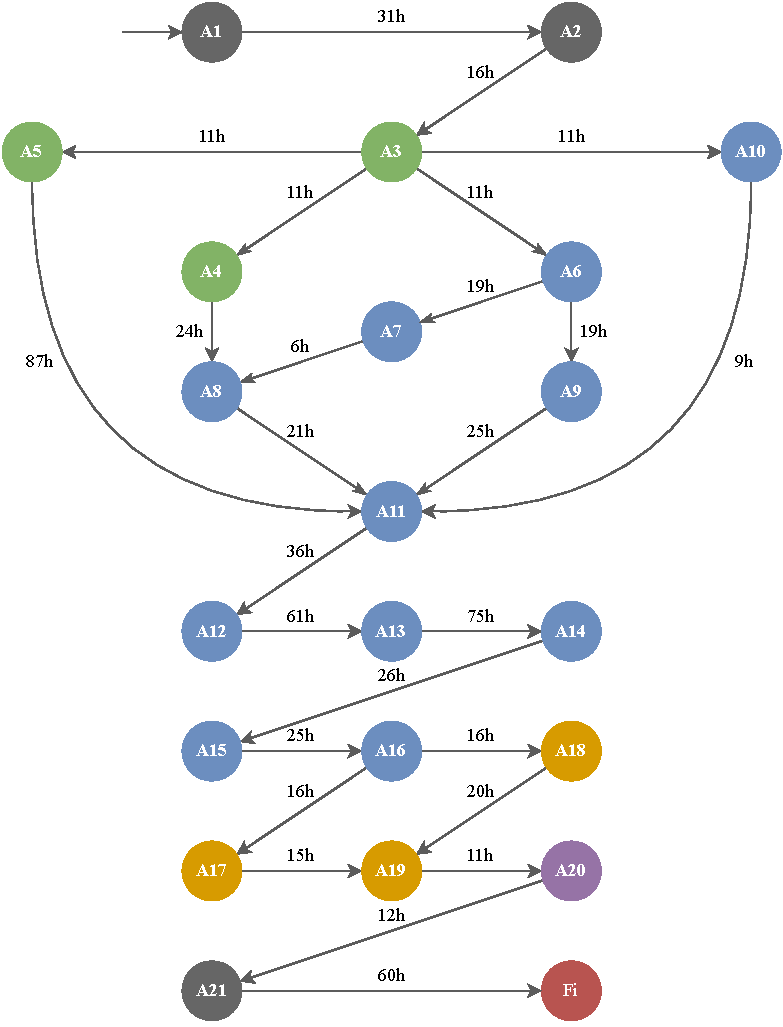
\includegraphics[width=0.88\textwidth]{assets/planification_figs/activityDiagram.pdf}
	\caption{\label{img:diagrama_activitats}Diagrama de les activitats planificades.}
\end{figure}

A partir del diagrama d'activitats, es pot saber fàcilment la durada màxima aproximada del projecte. Per calcular-la, cal sumar els temps de cadascuna de les activitats del camí crític del graf, és a dir, el camí des d'\texttt{A1} fins a \texttt{Fi} més costós en temps.

\textbf{A1} $\rightarrow$ \textbf{A2} $\rightarrow$ \textbf{A3} $\rightarrow$ \textbf{A5} $\rightarrow$ \textbf{A11} $\rightarrow$ \textbf{A12} $\rightarrow$ \textbf{A13} $\rightarrow$ \textbf{A14} $\rightarrow$ \textbf{A15} $\rightarrow$ \textbf{A16} $\rightarrow$ \textbf{A17} $\rightarrow$ \textbf{A19} $\rightarrow$ \textbf{A20} $\rightarrow$ \textbf{A21} $\rightarrow$ \textbf{Fi}

El resultat de la suma dels temps del camí crític i, per tant, la durada màxima estimada del projecte seria de 864 hores (669h de planificació i desenvolupament més 195h de documentació). No obstant això, aquest càlcul s'ha realitzat sense tenir en compte que el projecte es durà a terme de manera individual, ja que hi ha activitats que es poden realitzar paral·lelament.

Per tant, si es considera que les activitats no es paral·lelitzen, la durada màxima estimada del projecte és de \textbf{1055 hores} (860h de planificació i desenvolupament més 195h de documentació).

\newpage

\begin{landscape}

\subsection{Cronograma}
\label{subsec:cronograma}

En aquesta subsecció, es representarà el diagrama de Gantt que recull la planificació del projecte a partir de les activitats determinades a la subsecció~\ref{subsec:determinacio_activitats} i n'estima les dates (veure figura~\ref{img:diagrama_gantt}).

\begin{figure}[H]
  \centering
  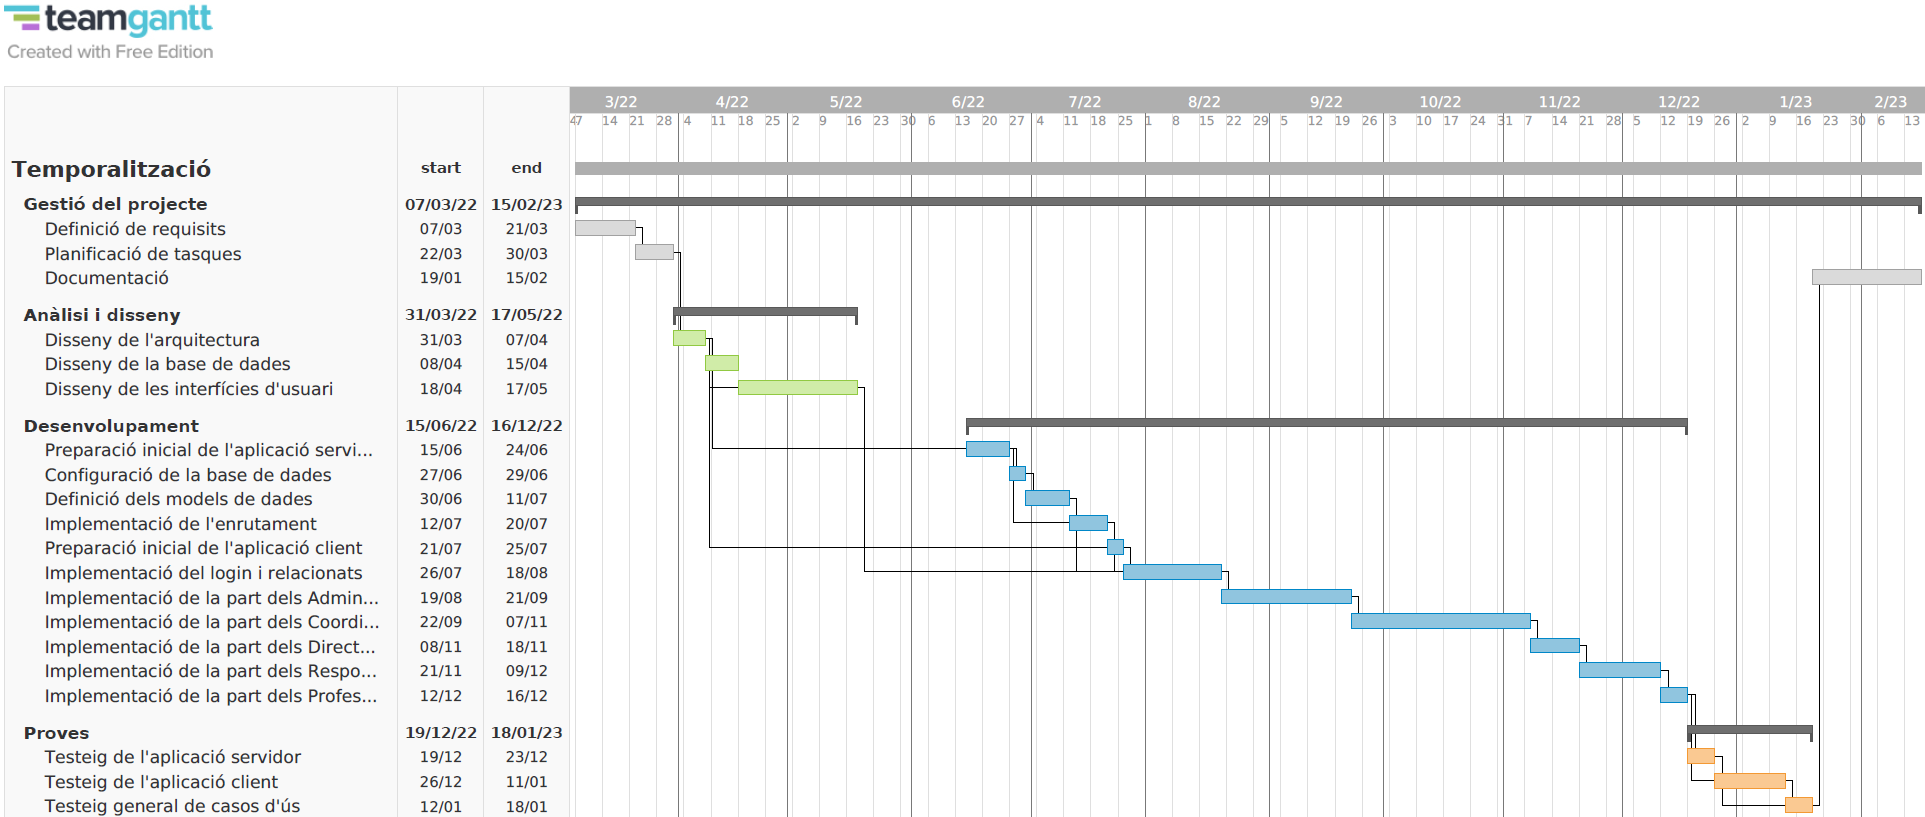
\includegraphics[width=1.5\textwidth]{assets/planification_figs/ganttDiagram.png}
  \caption{\label{img:diagrama_gantt}Diagrama de Gantt.}
\end{figure}

\end{landscape}

\chapter{Estudis i decisions}
\label{cap:estudi}

\section{Introducció i estructura}
\label{sec:estudi_intro}

En aquesta secció, s'introduirà el contingut de la resta del capítol i se'n detallarà l'estructura.

Primerament, es parlarà sobre com s'ha gestionat i estructurat el projecte en quant al codi (veure secció~\ref{sec:decisions_estructura}). Tot seguit, ja s'entrarà en detall en les tecnologies utilitzades pel desenvolupament del programari, tant de l'aplicació client com de l'aplicació servidor (veure seccions~\ref{sec:decisions_client} i~\ref{sec:decisions_servidor}, respectivament). També s'explicaran les decisions que involucren la base de dades (veure secció~\ref{sec:decisions_bdd}). Per últim, s'indicaran les eines que s'han fet servir tant pel desenvolupament del programari com per a la confecció de la memòria (veure seccions~\ref{sec:decisions_desenvolupament} i~\ref{sec:decisions_memoria}, respectivament)

\section{Gestió i estructuració del projecte}
\label{sec:decisions_estructura}

\subsection{Control de versions}
\label{subsec:decisions_estructura_versions}

En aquesta subsecció, es justificarà l'el·lecció del sistema de control de versions utilitzat en el projecte: \textbf{Git}.

Disposar d'un sistema de control de versions a l'hora de desenvolupar una aplicació aporta un gran nombre d'avantatges, d'entre els quals destaca la capacitat de consultar o restaurar estats antics del codi i la de bifurcar el desenvolupament.

\textbf{Git}~\cite{Git} (veure figura~\ref{img:logo_git}), és el sistema de control de versions més popular amb diferència i, encara que existeixin algunes alternatives, és la que més funcionalitats ofereix i l'opció preferida de la gran majoria de desenvolupadors. A banda d'aquests motius, Git és l'única eina d'aquesta tipologia amb què tinc experiència. 

\begin{figure}[H]
  \centering
  
\includegraphics[width=0.2\textwidth]{assets/logos/Git.png}
  \caption{\label{img:logo_git}Logotip de Git.}
\end{figure}

Normalment, l'ús de \textbf{Git} sol acompanyar-se de l'allotjament dels repositoris a una plataforma web dedicada a aquesta funció. Aquests tipus de plataforma permeten evitar la pèrdua accidental del codi d'un projecte, a banda d'aportar incomptables funcionalitats per al treball col·laboratiu, entre d'altres.

Hi ha diverses alternatives pel que fa a aquest tipus de plataforma, com ara \textbf{GitHub}, GitLab o BitBucket. No obstant això, l'opció escollida per al projecte és \textbf{GitHub}~\cite{GitHub} (veure figura~\ref{img:logo_github}), ja que la domino més que la resta i em sento més còmode treballant-hi.

\begin{figure}[H]
  \centering
  
\includegraphics[width=0.26\textwidth]{assets/logos/GitHub.png}
  \caption{\label{img:logo_github}Logotip de GitHub.}
\end{figure}

Per últim, esmentar que aquestes eines s'han fet servir tant pel programari com per a la memòria.

\subsection{Estructuració del projecte}
\label{subsec:decisions_estructura_estructura}

En aquesta subsecció, es justificarà l'el·lecció de l'estructura del sistema: \textbf{monorepositori}.

Tal com s'ha vist al capítol~\ref{cap:marcdetreball}, el projecte engloba el desenvolupament de dues apliacions: el client i el servidor. Aquestes aplicacions es poden estructurar de dues maneres diferents:
\begin{itemize}
  \item \texttt{Multirepositori:} Separar les dues aplicacions en respositoris diferents. 
  \item \texttt{\textbf{Monorepositori:}} Agrupar les dues aplicacions en el mateix repositori.
\end{itemize}

Els beneficis principals del multirepositori són que els repositoris individuals són més fàcils de gestionar i queden més nets i recollits. En canvi, encara que en el \textbf{monorepositori} passi el contrari, és un aspecte que no té gaire pes, ja que l'escala del projecte és petita. A més a més, aquesta alternativa ofereix avantatges més interessants, com ara una millor estandarització del codi i la possibilitat de la seva reutilització, entre d'altres.

A més a més, tal com es veurà a les seccions~\ref{sec:decisions_client} i~\ref{sec:decisions_servidor}, el llenguatge de programació amb què s'han desenvolupat les dues aplicacions és el mateix: JavaScript. Gràcies a això es pot utilitzar un mateix gestor de paquets per a les dues.

Els gestors de paquets de JavaScript actuals més populars també incorporen altres eines i utilitats que faciliten la gestió d'un \textbf{monorepositori} dividint-lo en diferents espais de treball. Permeten definir les dependències de cada espai de treball i també les comunes. Aquest fet fa que la instal·lació i actualització dels paquets sigui més ràpida i eficient que en el cas de l'estructuració del projecte en multirepositori. Per aquests motius i per comoditat, l'el·lecció per al projecte ha estat l'estructuració en \textbf{monorepositori}.

Pel que fa al gestor de paquets, s'ha optat per \textbf{npm}~\cite{npm} (veure figura~\ref{img:logo_npm}). Els motius d'aquesta el·lecció han estat, principalment, el coneixement previ de l'eina i que és el gestor de paquets estàndard de Node.js, l'entorn escollit per a l'aplicació servidor (veure secció~\ref{sec:decisions_servidor}).

\begin{figure}[H]
  \centering
  
\includegraphics[width=0.2\textwidth]{assets/logos/NPM.png}
  \caption{\label{img:logo_npm}Logotip de npm.}
\end{figure}

\section{Aplicació client}
\label{sec:decisions_client}

\subsection{\textit{Bundler}}
\label{subsec:decisions_client_bundler}

En aquesta subsecció, es justificarà l'el·lecció del \textit{bundler} utilitzat en l'aplicació client: \textbf{Vite}.

Tal com s'ha vist al capítol~\ref{cap:marcdetreball}, existeixen múltiples eines d'aquesta tipologia que empaqueten el codi de tots els fitxers o mòduls JavaScript per tal de poder ser enviats al navegador en una sola petició, com ara \textbf{Vite}, WebPack, Rollup o Parcel.

No obstant això, el codi font de les aplicacions \textit{front-end} modernes pot arribar a ser enorme a causa de l'ús de \textit{frameworks} i biblioteques. Aquest fet comporta, entre d'altres inconvenients, una mala experiència de desenvolupament, ja que, per exemple, si es fa servir HMR (\textit{hot module replacement}), les modificacions d'arxius poden tardar uns quants segons en veure's reflectides al navegador. A més a més, el temps d'espera necessari per posar en marxa un servidor de desenvolupament pot resultar excessivament llarg.

Gràcies als avenços en l'ecosistema, com ara la disponibilitat de mòduls ES al navegador de forma nativa, han sorgit noves eines que se n'aprofiten i corregeixen els problemes que presenten els \textit{bundlers} comentats anteriorment.

Degut a aquests motius i a que la documentació oficial del \textit{framework} escollit pel \textit{front-end} del projecte (veure subsecció~\ref{subsec:decisions_client_framework}) en recomana l'ús, s'ha triat \textbf{Vite}.

\textbf{Vite}~\cite{Vite} (veure figura~\ref{img:logo_vite}) és una eina de compilació l'objectiu de la qual és proporcionar una experiència de desenvolupament àgil per a projectes web moderns. Entre d'altres funcionalitats, incorpora un servidor de desenvolupament que permet, per exemple, un HMR extremadament ràpid.

\begin{figure}[H]
  \centering
  
\includegraphics[width=0.16\textwidth]{assets/logos/Vite.png}
  \caption{\label{img:logo_vite}Logotip de Vite.}
\end{figure}

\subsection{\textit{Framework}}
\label{subsec:decisions_client_framework}

En aquesta subsecció, es justificarà l'el·lecció del \textit{framework} JavaScript utilitzat en l'aplicació client: \textbf{Vue}.

Tal com s'ha vist al capítol~\ref{cap:marcdetreball}, els \textit{frameworks} més populars per a \textit{front-end} són React, Angular i \textbf{Vue}. Normalment, les tecnologies més populars són les que tenen una comunitat més gran i, per tant, n'existeix més documentació, més articles i més preguntes i respostes sobre quasi bé qualsevol tipus de problema o dubte. Per aquest motiu, d'entrada, l'el·lecció s'ha disputat entre aquests tres \textit{frameworks}.

No obstant això, Angular~\cite{Angular} ha estat la primera opció descartada. En comparació amb les altres alternatives, és la més pesada, més complexa i amb la corva d'aprenentatge més pronunciada, ja que disposa d'una gran quantitat d'eines i possibilitats que, en moltes ocasions, poden resultar excessives i agobiants a l'hora de desenvolupar aplicacions a petita o mitjana escala.

En aquest punt, s'ha realitzat una comparació entre React~\cite{React} i \textbf{Vue}~\cite{Vue} tenint en compte els avantatges i inconvenients principals de cadascun~\cite{ReactVsVue}.
\begin{itemize}
  \item Avantatges principals de React:
  \begin{itemize}
    \item Disposa d'una sintaxi pròpia que permet implementar més funcionalitat amb menys codi.
    \item No és difícil d'apendre per algú experimentat en JavaScript.
    \item S'ha desenvolupat un conjunt d'eines i utilitats que, en resum, faciliten molt la comprensió i depuració del codi.
  \end{itemize}
  \item Inconvenients principals de React:
  \begin{itemize}
    \item La documentació és bastant pobre, ja que el \textit{software} evoluciona a un ritme molt ràpid i no es dóna l'abast a l'hora de documentar-lo.
    \item Depèn molt d'altres eines que completen determinades funcionalitats que li falten.
    \item Degut a la ràpida evolució i actualització, molts desenvolupadors no es senten còmodes en haver d'estar aprenent continuament com es fan determinades coses que, cada poc temps, canvien de manera de fer.
  \end{itemize}
  \item Avantatges principals de \textbf{Vue}:
  \begin{itemize}
    \item És molt còmode de treballar-hi gràcies a la llegibilitat i simplicitat del codi.
    \item És molt lleguer, ja que només pesa 20KB.
    \item La documentació és molt completa i detallada, fet que el fa ràpid i senzill d'apendre per a desenvolupadors sense gaire experiència en aquest món.
    \item És capaç de detectar els components que contenen errors.
  \end{itemize}
  \item Inconvenients principals de \textbf{Vue}:
  \begin{itemize}
    \item És extremadament flexible, fet que facilita l'aparició d'irregularitats i errors.
    \item No disposa de gaires eines i utilitats comunes que ajuden a simplificar el desenvolupament.
  \end{itemize}
\end{itemize}

A l'hora de dur a terme la decisió final, s'ha valorat molt més l'opció més lleugera i que ofereix el codi més simple i llegible, la millor documentació i la corva d'aprenentatge menys pronunciada, ja que no tenia experiència prèvia en el desenvolupament d'aplicacions web. Per tant, \textbf{Vue} és el \textit{framework} escollit per a l'aplicació client del projecte.

\textbf{Vue} (veure figura~\ref{img:logo_vue}) és un \textit{framework} JavaScript per desenvolupar interfícies d'usuari. Està construit sobre HTML, CSS i JavaScript i proporciona un model de programació declaratiu basat en components.

\begin{figure}[H]
  \centering
  
\includegraphics[width=0.14\textwidth]{assets/logos/Vue.png}
  \caption{\label{img:logo_vue}Logotip de Vue.}
\end{figure}

El més comú és definir cada component en un fitxer diferent. Aquests fitxers utilitzen l'extensió ``.vue'' i se'ls anomena SFC (\textit{Single-File Component}). Cadascun està format per les tres parts principals següents:
\begin{itemize}
  \item \texttt{\textit{Script}}: Conté el codi JavaScript del component.
  \item \texttt{\textit{Template}}: Conté l'estructura HTML del component.
  \item \texttt{\textit{Style}}: Conté els estils CSS del component.
\end{itemize}

\subsection{Enrutament}
\label{subsec:decisions_client_enrutament}

En aquesta subsecció, es presentarà l'eina utilitzada per l'enrutament de l'aplicació client: \textbf{Vue Router}.

\textbf{Vue Router}~\cite{VueRouter} és l'enrutador oficial de Vue i està profundament integrat amb el seu nucli. Gràcies a aquesta utilitat, es poden implementar rutes dinàmiques, rutes basades en components, enrutament dinàmic, historial de rutes, etc.

\subsection{Gestió d'estats}
\label{subsec:decisions_client_estats}

En aquesta subsecció, es presentarà l'eina utilitzada per la gestió d'estats de l'aplicació client: \textbf{Pinia}.

\textbf{Pinia}~\cite{Pinia} (veure figura~\ref{img:logo_pinia}) és l'eina de gestió d'estats oficial de Vue i permet emmagatzemar i manipular dades reactives més enllà de la jerarquia de components i de manera global. A més a més, accepta HMR i disposa d'integracions amb les eines per a desenvolupadors dels navegadors.

\begin{figure}[H]
  \centering
  
\includegraphics[width=0.12\textwidth]{assets/logos/Pinia.png}
  \caption{\label{img:logo_pinia}Logotip de Pinia.}
\end{figure}

\subsection{Estètica i funcionalitats addicionals}
\label{subsec:decisions_client_estetica}

En aquesta subsecció, es presentaran les eines utilitzades en quant a estètica i en quant a l'aportació de funcionalitats addicionals que simplifiquen el desenvolupament de l'aplicació client i la fan més robusta: \textbf{Material Colors, Material Icons i Quasar}.

Material és un sistema de disseny que defineix unes guies d'estil enfocades al desenvolupament d'interfícies d'usuari d'alta qualitat. Per aquest motiu, abans de crear paletes de colors pròpies i buscar icones variades per al \textit{front-end} del projecte, es va optar per utilitzar \textbf{Material Colors}~\cite{MaterialColors} per escollir-ne les paletes de colors i \textbf{Material Icons}~\cite{MaterialIcons} per escollir-ne les icones.

L'abast de l'aplicació client és relativament gran i construir-la des de zero, tot i utilitzar un \textit{framework}, hagués suposat un cost temporal massa elevat. Per tal d'agilitzar-ne el desenvolupament, es va decidir incorporar al projecte alguna biblioteca que disposés de components reutilitzables útils i que seguíssin unes certes guies d'estil, com ara botons, seleccionables, etc.

L'alternativa més popular i més completa és Vuetify. No obstant això, aquesta eina encara no suporta l'última versió de Vue (Vue 3) i ha estat descartada. La segona millor opció després de Vuetify és \textbf{Quasar} i, encara que no sigui tant completa, ofereix components i funcionalitats molt útils i interessants.

\textbf{Quasar}~\cite{Quasar} (veure figura~\ref{img:logo_quasar}) és un \textit{framework} de codi obert basat en Vue. Encara que normalment s'utilitzi com a \textit{framework} ``principal'' d'un projecte, també es pot incorporar a un projecte existent creat amb Vite en forma de \textit{plugin}, com el cas de l'aplicació client d'aquest projecte.

\begin{figure}[H]
  \centering
  
\includegraphics[width=0.15\textwidth]{assets/logos/Quasar.png}
  \caption{\label{img:logo_quasar}Logotip de Quasar.}
\end{figure}

A continuació s'enumeren algunes de les funcionalitats que incorpora:
\begin{itemize}
  \item Components reutilitzables que van des de botons fins a taules complexes, arbres, etc.
  \item Classes CSS globals i possibilitat de definició de variables CSS.
  \item Eines (\textit{directives}) de Vue que permeten controlar events de ratolí, entre d'altres utilitats.
  \item Eines (\textit{composables}) de Vue que faciliten la separació i reutilització de diàlegs, entre d'altres utilitats.
  \item Suport per biblioteques d'icones com, per exemple, \textbf{Material Icons}.
\end{itemize}

\subsection{Proves}
\label{subsec:decisions_client_proves}

En aquesta subsecció, es presentaran les eines utilitzades per a la realització de proves a l'aplicació client: \textbf{Chrome DevTools amb una extensió de Vue}.

\textbf{Chrome DevTools}~\cite{ChromeDevTools} (veure figura~\ref{img:logo_chrome_dev_tools}) és un conjunt d'eines per a desenvolupadors que proporciona el navegador Google Chrome. Aquestes eines resulten molt útils a l'hora de comprovar que el \textit{software} funcioni i depurar-lo en cas que es produeixi algun error.

\begin{figure}[H]
  \centering
  
\includegraphics[width=0.22\textwidth]{assets/logos/ChromeDevTools.png}
  \caption{\label{img:logo_chrome_dev_tools}Logotip de Chrome DevTools.}
\end{figure}

A més a més, Vue disposa d'una extensió que s'afegeix a aquestes eines i fa possible la realització de proves i depuració molt més específiques.

\section{Aplicació servidor}
\label{sec:decisions_servidor}

\subsection{Entorn i llenguatge de programació}
\label{subsec:decisions_servidor_entorn}
En aquesta subsecció, es justificarà l'el·lecció tant de l'entorn com del llenguatge de programació utilitzats en l'aplicació servidor: \textbf{JavaScript en l'entorn de Node.js}.

Tal com s'ha vist al capítol~\ref{cap:marcdetreball}, existeix una quantitat considerable d'entorns i llenguatges de programació que permeten desenvolupar aplicacions de \textit{back-end}. D'entrada i per raons de temps, es descarten els llenguatges amb els quals no tinc cap tipus d'experiència.

En aquest punt, les dues alternatives són \textbf{JavaScript en l'entorn de Node.js} i Java. Les aplicacions servidor desenvolupades amb Java són una bona opció però, en notables ocasions, els seus \textit{frameworks} comporten una configuració excessiva que requereix bastant temps i pot dur a errors. D'altra banda, els \textit{frameworks} \textbf{JavaScript} que funcionen sobre \textbf{Node.js} solen ser molt més lleugers i senzills de fer servir a nivell bàsic. A més a més, \textbf{JavaScript} és el llenguatge que més m'interessa apendre actualment.

Per aquests motius i per evitar la incomoditat d'haver de desenvolupar a la vegada dues aplicacions amb llenguatges diferents, l'alternativa escollida ha estat \textbf{JavaScript en l'entorn de Node.js}.

\textbf{Node.js}~\cite{Node} (veure figura~\ref{img:logo_node}) és un entorn d'execució de \textbf{JavaScript} multiplataforma i de codi obert que funciona fora del navegador i està orientat al processament d'events asíncrons. Està dissenyat principalment per crear aplicacions de xarxa escalables. L'escalabilitat és possible gràcies a la seva capacitat d'atendre múltiples connexions simultàniament sense cap possibilitat de bloqueig: utilitza un sol fil d'execució, el qual executa una funció (\textit{callback}) per a cada connexió. Si aquesta funció realitza una operació asíncrona, com ara comunicar-se amb un sistema gestor de bases de dades, \textbf{Node.js} no es bloqueja mentre espera que finalitzi l'operació, sinó que n'executa d'altres que tingui pendents, com per exemple atendre una altra connexió. No obstant això, un cop hagi acabat l'operació, continuarà amb l'execució de la funció.

\begin{figure}[H]
  \centering
  
\includegraphics[width=0.24\textwidth]{assets/logos/Node.png}
  \caption{\label{img:logo_node}Logotip de Node.js.}
\end{figure}

\subsection{\textit{Framework}}
\label{subsec:decisions_servidor_framework}

En aquesta subsecció, es presentarà el \textit{framework} JavaScript utilitzat en l'aplicació servidor: \textbf{Express.js}.

\textbf{Express.js}~\cite{Express} (veure figura~\ref{img:logo_express}) és el \textit{framework} JavaScript que funciona sobre Node.js més popular. Destaca per ser molt lleuger, minimalista i flexible, a més de proporcionar una metodologia ràpida per crear API REST.

\begin{figure}[H]
  \centering
  
\includegraphics[width=0.24\textwidth]{assets/logos/Express.png}
  \caption{\label{img:logo_express}Logotip d'Express.js.}
\end{figure}

\subsection{ORM}
\label{subsec:decisions_servidor_orm}

En aquesta subsecció, es presentarà l'ORM utilitzat en l'aplicació servidor: \textbf{Sequelize}.

Un ORM (\textit{object relational mapper}) és una tècnica o patró arquitectònic que permet comunicar l'aplicació servidor amb un sistema gestor de bases de dades. La seva finalitat és crear models virtuals per a cada taula de la base de dades i generar comandes SQL automàticament a partir d'instruccions executades amb el llenguatge de l'apliació.

\textbf{Sequelize}~\cite{Sequelize} (veure figura~\ref{img:logo_sequelize}) és un ORM desenvolupat per a Node.js que suporta treballar amb diversos SGBD: PostgreSQL, MySQL, SQLite i MSSQL. Ofereix un ampli conjunt de funcionalitats, les principals del qual són: fort suport de transaccions, relacions, múltiples maneres de carregar dades, esborrat no definitiu, etc.

\begin{figure}[H]
  \centering
  
\includegraphics[width=0.25\textwidth]{assets/logos/Sequelize.png}
  \caption{\label{img:logo_sequelize}Logotip de Sequelize.}
\end{figure}

\subsection{Proves}
\label{subsec:decisions_servidor_proves}

En aquesta subsecció, es justificarà l'el·lecció de l'eina utilitzada per a la realització de proves a l'API que exposa l'aplicació servidor: \textbf{Postman}.

Les dues alternatives que possibiliten realitzar aquestes proves més conegudes són \textbf{Postman} i Insomnia. Pel que fa a aquest projecte, les dues eines són igual d'útils i ofereixen quasi bé les mateixes possibilitats.

No obstant això, l'opció amb la qual tinc més experiència és \textbf{Postman} i, per tant, és l'escollida.

\textbf{Postman}~\cite{Postman} (veure figura~\ref{img:logo_postman}) és una plataforma d'API per a desenvolupadors que serveix per dissenyar i comprovar el funcionament de les API.

\begin{figure}[H]
  \centering
  
\includegraphics[width=0.23\textwidth]{assets/logos/Postman.png}
  \caption{\label{img:logo_postman}Logotip de Postman.}
\end{figure}

\section{Base de dades}
\label{sec:decisions_bdd}

\subsection{Entorn d'execució}
\label{subsec:decisions_bdd_entorn}

En aquesta subsecció, es justificarà l'el·lecció de l'entorn d'execució sobre el qual s'executa l'SGBD del projecte: \textbf{Docker}.

Abans d'instal·lar i fer servir un SGBD directament sobre el sistema operatiu de l'ordinador personal, s'ha optat per fer-ho en un entorn que cada vegada és més popular i que ofereix nombrosos avantatges: \textbf{Docker}.

\textbf{Docker}~\cite{Docker} (veure figura~\ref{img:logo_docker}) és un \textit{software} de codi obert que automatitza el desplegament d'aplicacions dins de contenidors construïts sobre el nucli de Linux. Permet disposar d'imatges predefinides d'un determinat aplicatiu per tal de poder executar-les fàcilment, com ara la imatge d'un SGBD. El punt clau d'això és que un contenidor pot allotjar un determinat programari i tota la seva configuració, de manera que tot plegat sigui portable i ràpidament executable en altres màquines i sistemes operatius.

\begin{figure}[H]
  \centering
  
\includegraphics[width=0.25\textwidth]{assets/logos/Docker.png}
  \caption{\label{img:logo_docker}Logotip de Docker.}
\end{figure}

\subsection{Sistema gestor de bases de dades}
\label{subsec:decisions_bdd_sgbd}

En aquesta subsecció, es justificarà l'el·lecció del sistema gestor de bases de dades utilitzat per gestionar les dades del projecte: \textbf{MySQL}.

Per començar, si s'analitzen mínimament el tipus de dades que involucra el projecte, ràpidament es pot concloure que l'opció més òptima és decantar-se per una base de dades relacional, ja que estan molt relacionades entre sí.

Els SGBD relacionals més populars i més ben documentats són Oracle, \textbf{MySQL}, Microsoft SQL Server i PostgreSQL. No obstant això, les dues opcions candidates són Oracle i \textbf{MySQL}, ja que són les úniques amb les quals tinc experiència.

Tal com s'ha vist a la secció~\ref{sec:decisions_servidor}, l'ORM escollit per al projecte funciona només amb un conjunt limitat de SGBD, el qual no contempla Oracle. Per tant, el sistema gestor de bases de dades escollit és \textbf{MySQL}.

\textbf{MySQL}~\cite{MySQL} (veure figura~\ref{img:logo_mysql}) és un sistema gestor de bases de dades relacional de codi lliure i multiusuari que funciona amb múltiples fils d'execució i utilitza el llenguatge SQL.

\begin{figure}[H]
  \centering
  
\includegraphics[width=0.2\textwidth]{assets/logos/MySQL.png}
  \caption{\label{img:logo_mysql}Logotip de MySQL.}
\end{figure}

\subsection{Proves}
\label{subsec:decisions_bdd_proves}

En aquesta subsecció, es justificarà l'el·lecció de l'eina utilitzada per a la realització de proves en quant a la base de dades: \textbf{DataGrip}.

Existeixen diverses opcions que permeten verificar el correcte ús d'una base de dades gestionada, en el cas d'aquest projecte, per MySQL (veure subsecció~\ref{subsec:decisions_bdd_sgbd}): mitjançant comandes directament a una consola o utilitzant un programari específic com ara MySQL Workbench o \textbf{DataGrip}.

Tot i tenir experiència amb MySQL Workbench, m'he decantat per \textbf{DataGrip} perquè l'he trobat molt més agradable visualment, més còmode i, sobretot, més potent, ja que ofereix més funcionalitats.

\textbf{DataGrip}~\cite{DataGrip} (veure figura~\ref{img:logo_datagrip}) és un entorn de desenvolupament integrat que permet treballar amb bases de dades i SQL. Permet guardar consultes, modificar dades i generar diagrames, entre moltes altres funcionalitats. A més a més, és compatible amb un gran nombre de SGBD.

\begin{figure}[H]
  \centering
  
\includegraphics[width=0.13\textwidth]{assets/logos/DataGrip.png}
  \caption{\label{img:logo_datagrip}Logotip de DataGrip.}
\end{figure}

\section{Eines de desenvolupament}
\label{sec:decisions_desenvolupament}

\subsection{Editor de codi}
\label{subsec:decisions_desenvolupament_editor}

En aquesta subsecció, es presentarà l'editor de codi amb què s'ha desenvolupat el projecte: \textbf{Visual Studio Code}.

\textbf{Visual Studio Code}~\cite{VSCode} (veure figura~\ref{img:logo_vscode}) és un editor de codi font molt lleuger i extremadament flexible i configurable. Gràcies a les seves extensions, es pot utilitzar per desenvolupar codi en qualsevol llenguatge de programació i per obrir i interpretar una gran quantitat de tipus de fitxer.

\begin{figure}[H]
  \centering
  
\includegraphics[width=0.15\textwidth]{assets/logos/VSCode.png}
  \caption{\label{img:logo_vscode}Logotip de Visual Studio Code.}
\end{figure}

Aquest editor ha resultat extremadament útil durant el desenvolupament del projecte, ja que s'ha pogut utilitzar tant pel codi font del \textit{front-end} i el \textit{back-end} com pel codi de la memòria, escrit amb LaTeX (veure secció~\ref{sec:decisions_memoria}).

\section{Confecció de la memòria}
\label{sec:decisions_memoria}

\subsection{Elaboració del document}
\label{subsec:decisions_memoria_document}

En aquesta subsecció, es presentarà l'eina utilitzada per a l'elaboració de la memòria del projecte: \textbf{LaTeX}.

\textbf{LaTeX}~\cite{LaTeX} (veure figura~\ref{img:logo_latex}) és un sistema de composició de textos orientat a la creació de documents escrits que han de presentar una alta qualitat tipogràfica. Degut a les seves característiques, és molt utilitzat en articles i llibres científics, tesis tècniques, etc.

\begin{figure}[H]
  \centering
  
\includegraphics[width=0.27\textwidth]{assets/logos/LaTeX.png}
  \caption{\label{img:logo_latex}Logotip de LaTeX.}
\end{figure}

\subsection{Disseny de les figures}
\label{subsec:decisions_memoria_figures}

En aquesta subsecció, es presentarà l'eina utilitzada per a l'elaboració de les figures presentades a la memòria: \textbf{Diagrams.net}.

\textbf{Diagrams.net}~\cite{DiagramsNet} (veure figura~\ref{img:logo_diagrams}) és una eina de codi obert que permet crear una gran varietat d'esquemes i diagrames de qualsevol mena. Per exemple, es fa servir molt freqüentment per dibuixar diagrames UML.

\begin{figure}[H]
  \centering
  
\includegraphics[width=0.13\textwidth]{assets/logos/diagramsNet.png}
  \caption{\label{img:logo_diagrams}Logotip de Diagrams.net.}
\end{figure}

\subsection{Diagrama de Gantt}
\label{subsec:decisions_memoria_gantt}

En aquesta subsecció, es presentarà l'eina utilitzada per a l'elaboració del diagrama de Gantt presentat a la memòria (veure capítol~\ref{cap:planificacio}): \textbf{TeamGantt}.

\textbf{TeamGantt}~\cite{TeamGantt} (veure figura~\ref{img:logo_teamGantt}) és una plataforma web que permet confeccionar diagrames de Gantt atractius i de manera relativament còmode.

\begin{figure}[H]
  \centering
  
\includegraphics[width=0.25\textwidth]{assets/logos/teamGantt.png}
  \caption{\label{img:logo_teamGantt}Logotip de Teamgantt.}
\end{figure}


\chapter{Anàlisi i disseny del sistema}
\label{cap:analisi}

\section{Anàlisi dels casos d'ús}
\label{sec:casos_us}

\subsection{Actors implicats}
\label{subsec:casos_us_actors}

En aquesta subsecció, es recolliran els actors que poden interactuar amb l'aplicació de manera externa. També s'indicaran les relacions d'especialització / generalització que estableixen.

Tal com es pot veure a la figura~\ref{img:casos_us_actors}, els actors corresponen als diferents rols d'usuari que participen en l'aplicació. Tots aquests actors, que disposen del seu propi conjunt d'interaccions possibles amb el sistema, també hereten el d'\emph{Usuari}, ja que en són especialitzacions.

\begin{figure}[H]
  \centering
  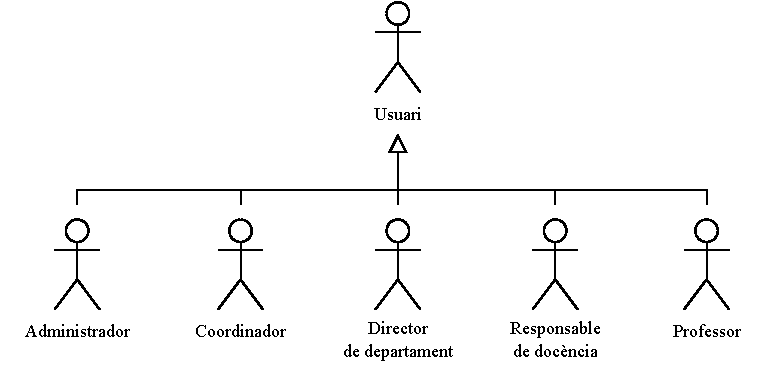
\includegraphics[width=\textwidth]{assets/use_cases/actors.pdf}
  \caption{\label{img:casos_us_actors}Jerarquia d'actors que poden interactuar amb l'aplicació.}
\end{figure}

\newpage

\subsection{Autenticació}
\label{subsec:casos_us_auth}

En aquesta subsecció, es representaran els casos d'ús relacionats amb la part de l'autenticació d'usuaris (veure figura~\ref{img:casos_us_auth}).

Quan es parli d'un \textit{Token}, s'estarà fent referència a un \textit{JSON Web Token}~\cite{JWT} generat per codificar certes dades amb una finalitat concreta (més informació sobre la implementació al capítol~\ref{cap:implementacio}).

\begin{figure}[H]
  \centering
  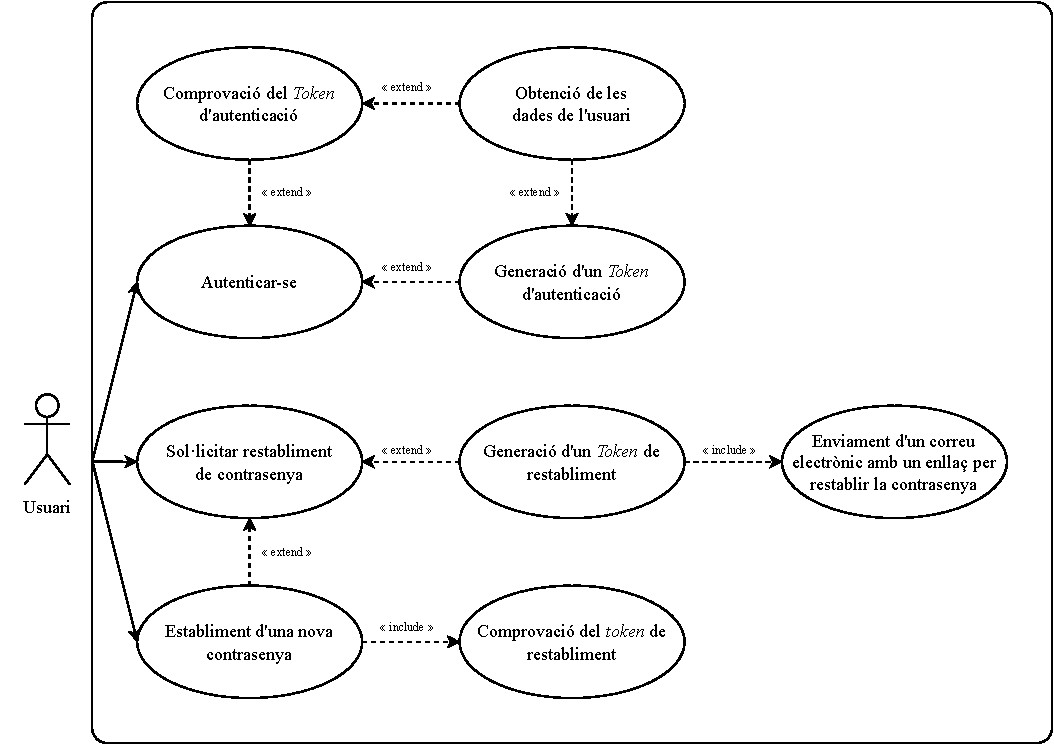
\includegraphics[width=\textwidth]{assets/use_cases/auth.pdf}
  \caption{\label{img:casos_us_auth}Diagrama dels casos d'ús relacionats amb l'autenticació.}
\end{figure}

\newpage

\subsection{Gestió del pla docent}
\label{subsec:casos_us_pla}

\subsubsection{General}

En aquest apartat, es representaran els casos d'ús generals involucrats en la gestió del pla docent (veure figura~\ref{img:casos_us_pla_general}), els quals seran desglossats en els apartats posteriors de la subsecció.

\begin{figure}[H]
  \centering
  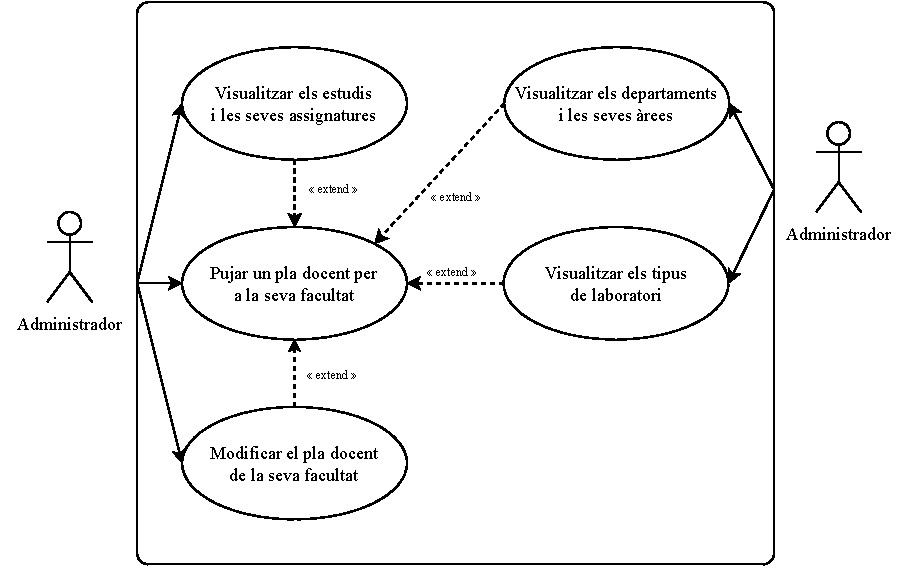
\includegraphics[width=0.9\textwidth]{assets/use_cases/pla_docent/general.pdf}
  \caption{\label{img:casos_us_pla_general}Diagrama de casos d'ús general de la gestió del pla docent.}
\end{figure}

\newpage

\subsubsection{Pujada d'un pla docent}

En aquest apartat, es representaran els casos d'ús involucrats en la pujada d'un pla docent (veure figura~\ref{img:casos_us_pla_pujada}).

\begin{figure}[H]
  \centering
  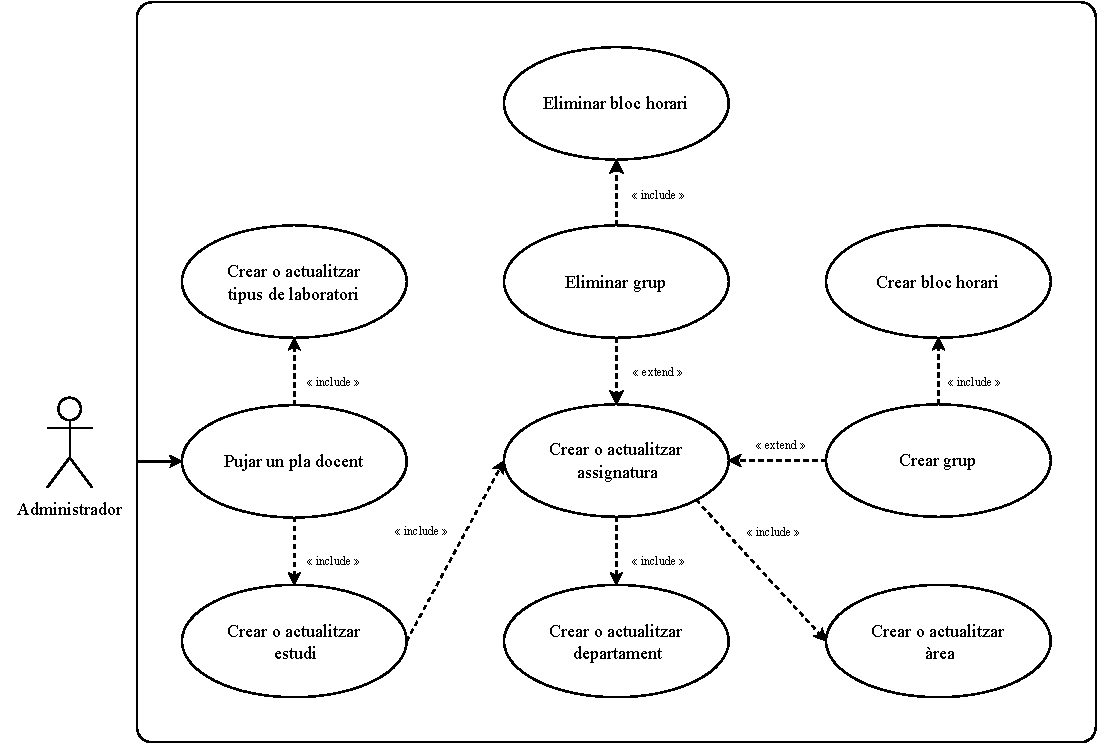
\includegraphics[width=\textwidth]{assets/use_cases/pla_docent/pujada.pdf}
  \caption{\label{img:casos_us_pla_pujada}Diagrama de casos d'ús de la pujada d'un pla docent.}
\end{figure}

\newpage

\subsubsection{Modificació del pla docent}

En aquest apartat, es representaran els casos d'ús involucrats en la modificació d'un pla docent (veure figura~\ref{img:casos_us_pla_modif}).

\begin{figure}[H]
  \centering
  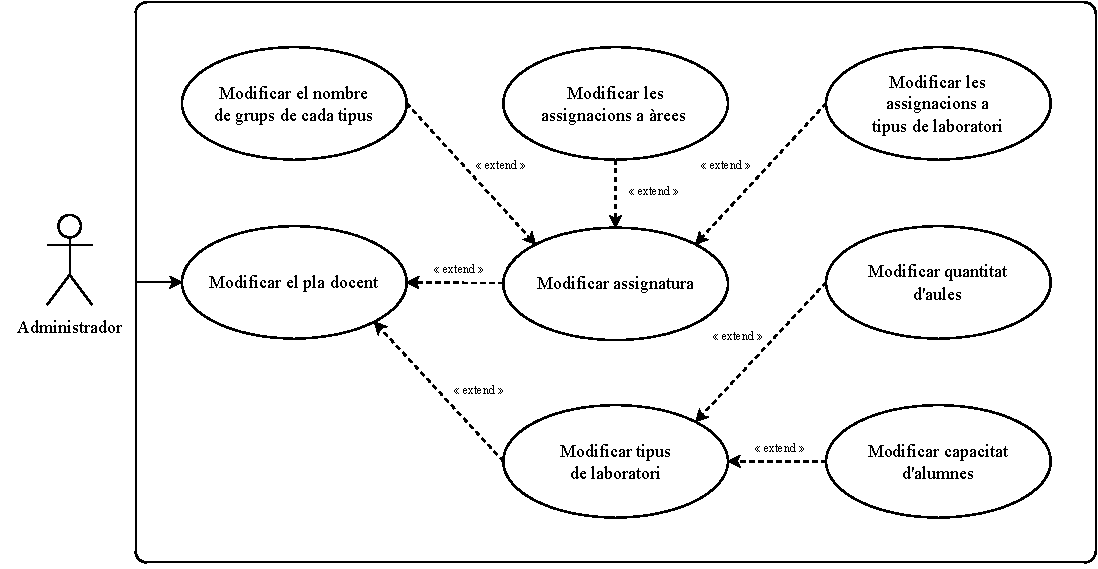
\includegraphics[width=\textwidth]{assets/use_cases/pla_docent/modif.pdf}
  \caption{\label{img:casos_us_pla_modif}Diagrama de casos d'ús de la modificació del pla docent.}
\end{figure}

\newpage

\subsection{Gestió d'usuaris}
\label{subsec:casos_us_usuaris}

En aquesta subsecció, es representaran els casos d'ús involucrats en la gestió d'usuaris (veure figura~\ref{img:casos_us_usuaris}).

És important destacar que, per motius de llegibilitat, s'ha optat per representar només una vegada i de manera genèrica els casos d'ús ``Crear usuari'', ``Eliminar usuari'' i ``Reenviar correu d'activació''.

En realitat, aquests casos d'ús només s'apliquen a un usuari d'un rol concret, el qual és definit segons el rol dels usuaris que s'estiguin gestionant: en la gestió de Coordinadors, només s'apliquen a usuaris Coordinadors i així successivament.

\begin{figure}[H]
  \centering
  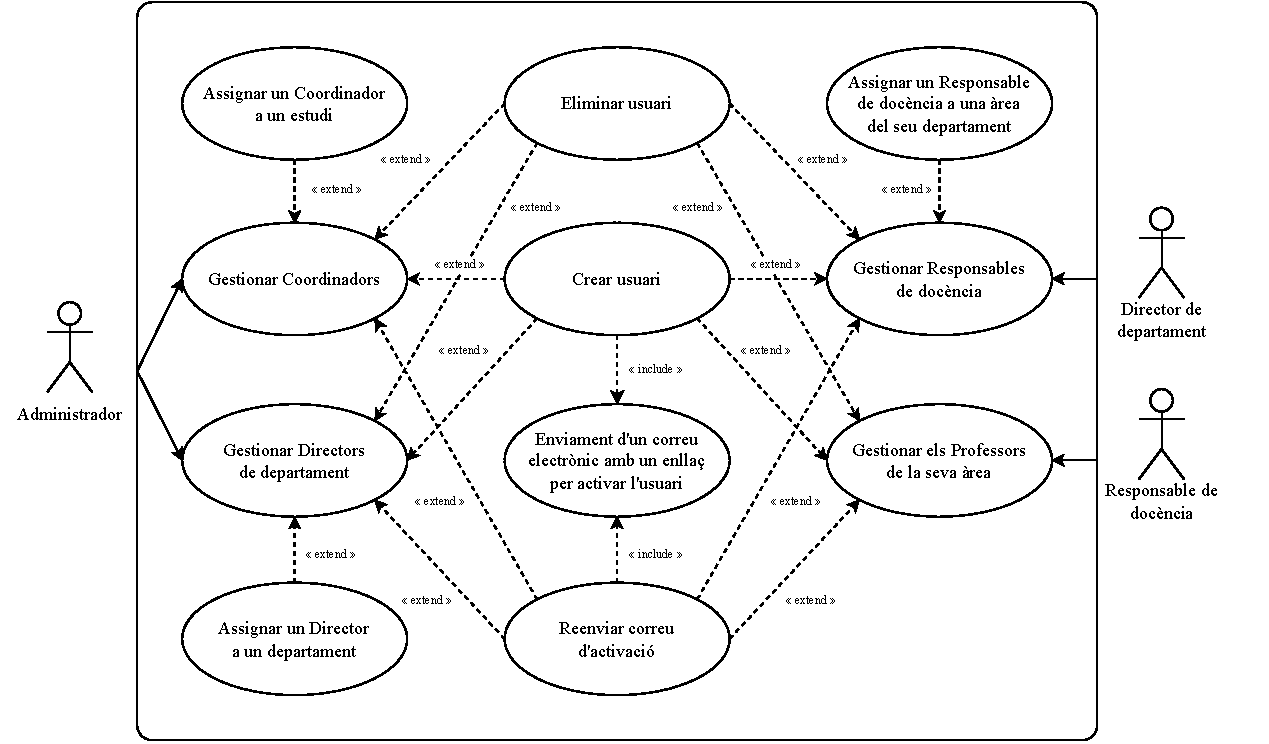
\includegraphics[width=\textwidth]{assets/use_cases/usuaris.pdf}
  \caption{\label{img:casos_us_usuaris}Diagrama de casos d'ús de la gestió d'usuaris.}
\end{figure}

\newpage

\subsection{Visualització d'horaris}
\label{subsec:casos_us_veure_horaris}

En aquesta subsecció, es representaran els casos d'ús involucrats en la visualització d'horaris (veure figura~\ref{img:casos_us_veure_horaris}).

\begin{figure}[H]
  \centering
  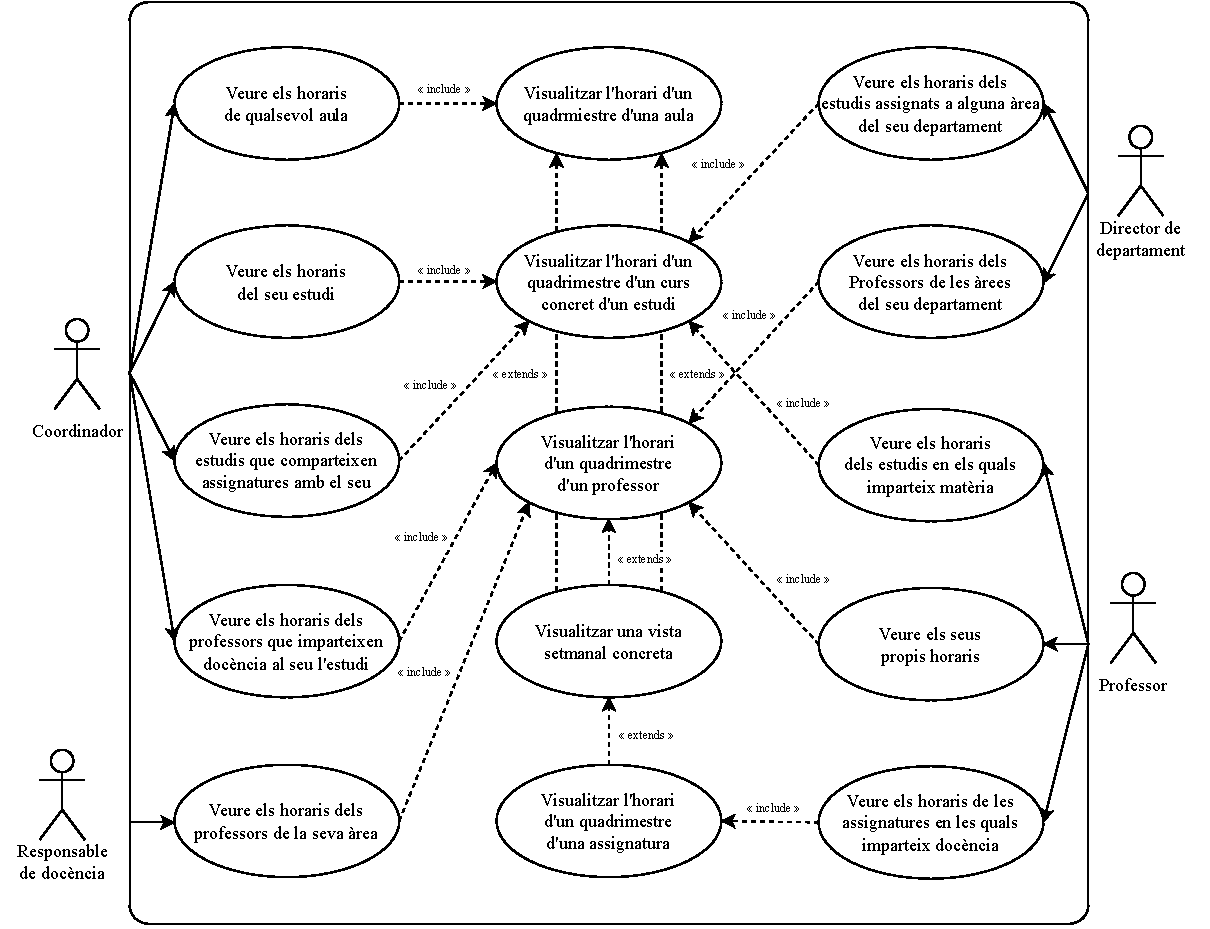
\includegraphics[width=\textwidth]{assets/use_cases/horaris/visualitzar.pdf}
  \caption{\label{img:casos_us_veure_horaris}Diagrama de casos d'ús de la visualització d'horaris.}
\end{figure}

\newpage

\subsection{Modificació d'horaris d'estudis}
\label{subsec:casos_us_modif_horaris}

\subsubsection{General}

En aquest apartat, es representaran els casos d'ús generals involucrats en la modificació dels horaris dels estudis (veure figura~\ref{img:casos_us_modif_horaris_general}), els quals seran desglossats en els apartats posteriors de la subsecció.

\begin{figure}[H]
  \centering
  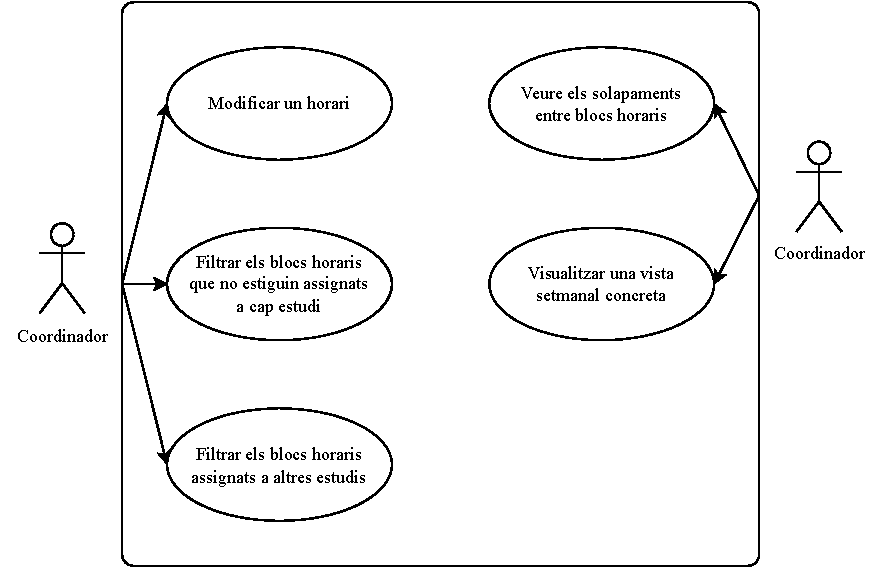
\includegraphics[width=0.9\textwidth]{assets/use_cases/horaris/modificar/general.pdf}
  \caption{\label{img:casos_us_modif_horaris_general}Diagrama de casos d'ús general de la modificació d'horaris.}
\end{figure}

\newpage

\subsubsection{Modificació d'un horari d'un estudi}

En aquest apartat, es representaran els casos d'ús involucrats en la modificació d'un horari d'un estudi (veure figura~\ref{img:casos_us_horaris_modif}).

És important destacar que el cas d'ús ``Modificar un horari del seu estudi'' es refereix a la modificació de l'horari d'un quadrimestre d'un dels cursos de l'estudi que gestiona el Coordinador en qüestió.

A més a més, cal afegir que, per motius de llegibilitat, s'ha optat per representar només una vegada i de manera genèrica el cas d'ús ``Modificar dades relacionades amb el temps'', ja que serveix tant per blocs horaris com per blocs horaris genèrics.

\begin{figure}[H]
  \centering
  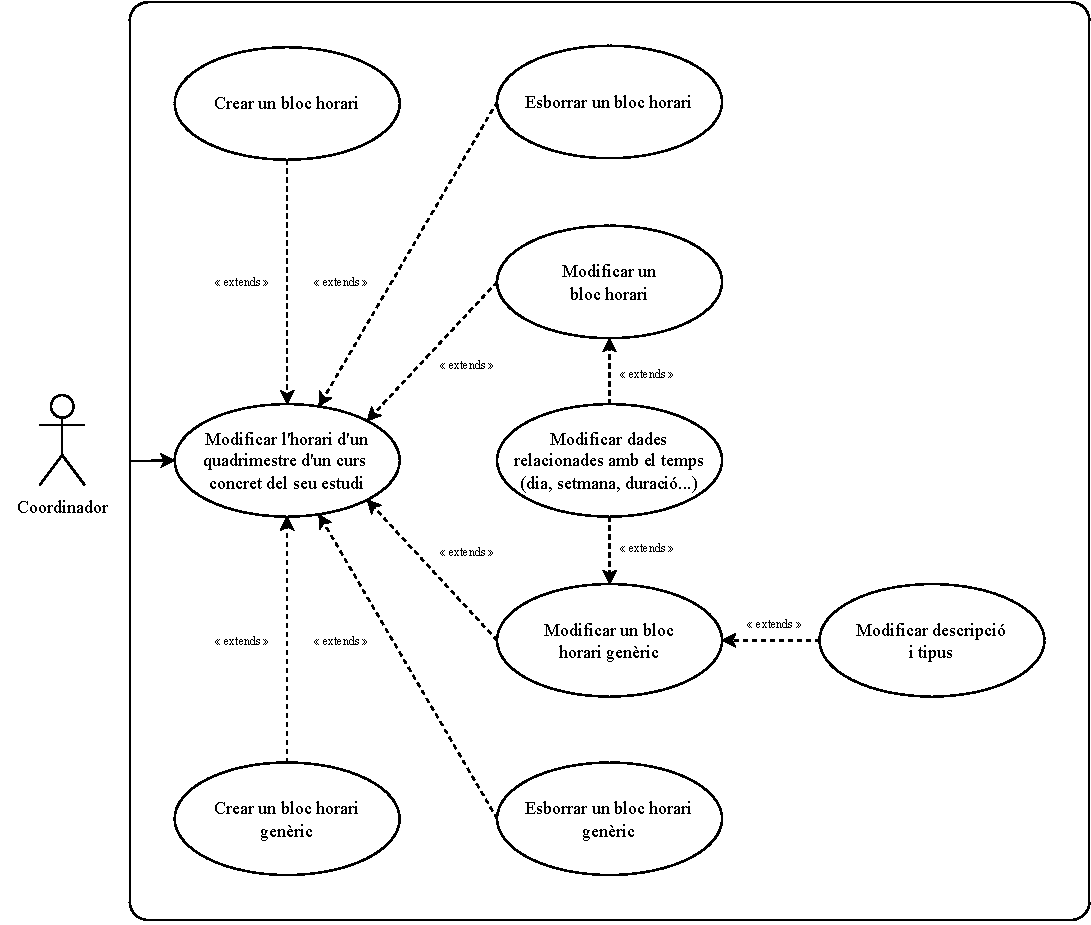
\includegraphics[width=\textwidth]{assets/use_cases/horaris/modificar/modif.pdf}
  \caption{\label{img:casos_us_horaris_modif}Diagrama de casos d'ús de la modificació d'un horari d'un estudi.}
\end{figure}

\newpage

\subsubsection{Visualització de solapaments}

En aquest apartat, es representaran els casos d'ús involucrats en la visualització de solapaments entre blocs horaris (veure figura~\ref{img:casos_us_horaris_solap}).

És important destacar que el cas d'ús ``Veure els solapaments entre blocs horaris'' es refereix als solapaments existents a l'horari d'un quadrimestre d'un dels cursos de l'estudi que gestiona el Coordinador en qüestió.

\begin{figure}[H]
  \centering
  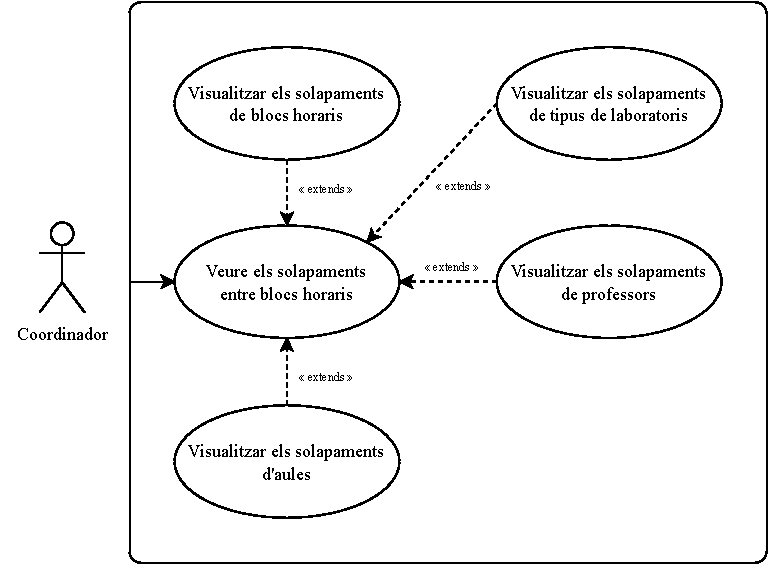
\includegraphics[width=0.9\textwidth]{assets/use_cases/horaris/modificar/solapaments.pdf}
  \caption{\label{img:casos_us_horaris_solap}Diagrama de casos d'ús de la visualització de solapaments.}
\end{figure}

\newpage

\section{Disseny de la base de dades}
\label{sec:disseny_bdd}

\subsection{Model entitat-relació}
\label{subsec:bd_model_er}

En aquesta subsecció, es presentarà el diagrama entitat-relació dissenyat per emmagatzemar i gestionar adequadament les dades de l'aplicació (veure figura~\ref{img:db}).

Per tal d'evitar la rectificació manual del diagrama davant de qualsevol canvi en el disseny, s'ha optat per utilitzar una eina que en permeti la generació automàtica a partir de les taules que formin la base de dades. Més concretament, es tracta de DataGrip~\cite{DataGrip}.

La part negativa d'aquest programa és que no explicita la cardinalitat de les relacions. Per aquest motiu, és molt important remarcar que totes les relacions són ``u a molts'' exceptuant les següents que són ``u a u'':
\begin{itemize}
  \item \texttt{Estudi} (0..1) $\longrightarrow$ (0..1) \texttt{Usuari}.
  \item \texttt{Departament} (0..1) $\longrightarrow$ (0..1) \texttt{Usuari}.
  \item \texttt{Àrea} (0..1) $\longrightarrow$ (0..1) \texttt{Usuari}.
\end{itemize}

També cal tenir en compte que les relacions ``molts a molts'' hi apareixen ja ``aplicades'' amb la taula intermitja entre les dues entitats en qüestió, la qual és necessària per a la seva implementació. A més a més, l'herència d'usuaris també hi apareix ``resolta'' amb una implementació concreta (veure capítol~\ref{cap:estudi} per conèixer els detalls d'aquesta decisió).

\newpage

\begin{figure}[H]
	\centering
	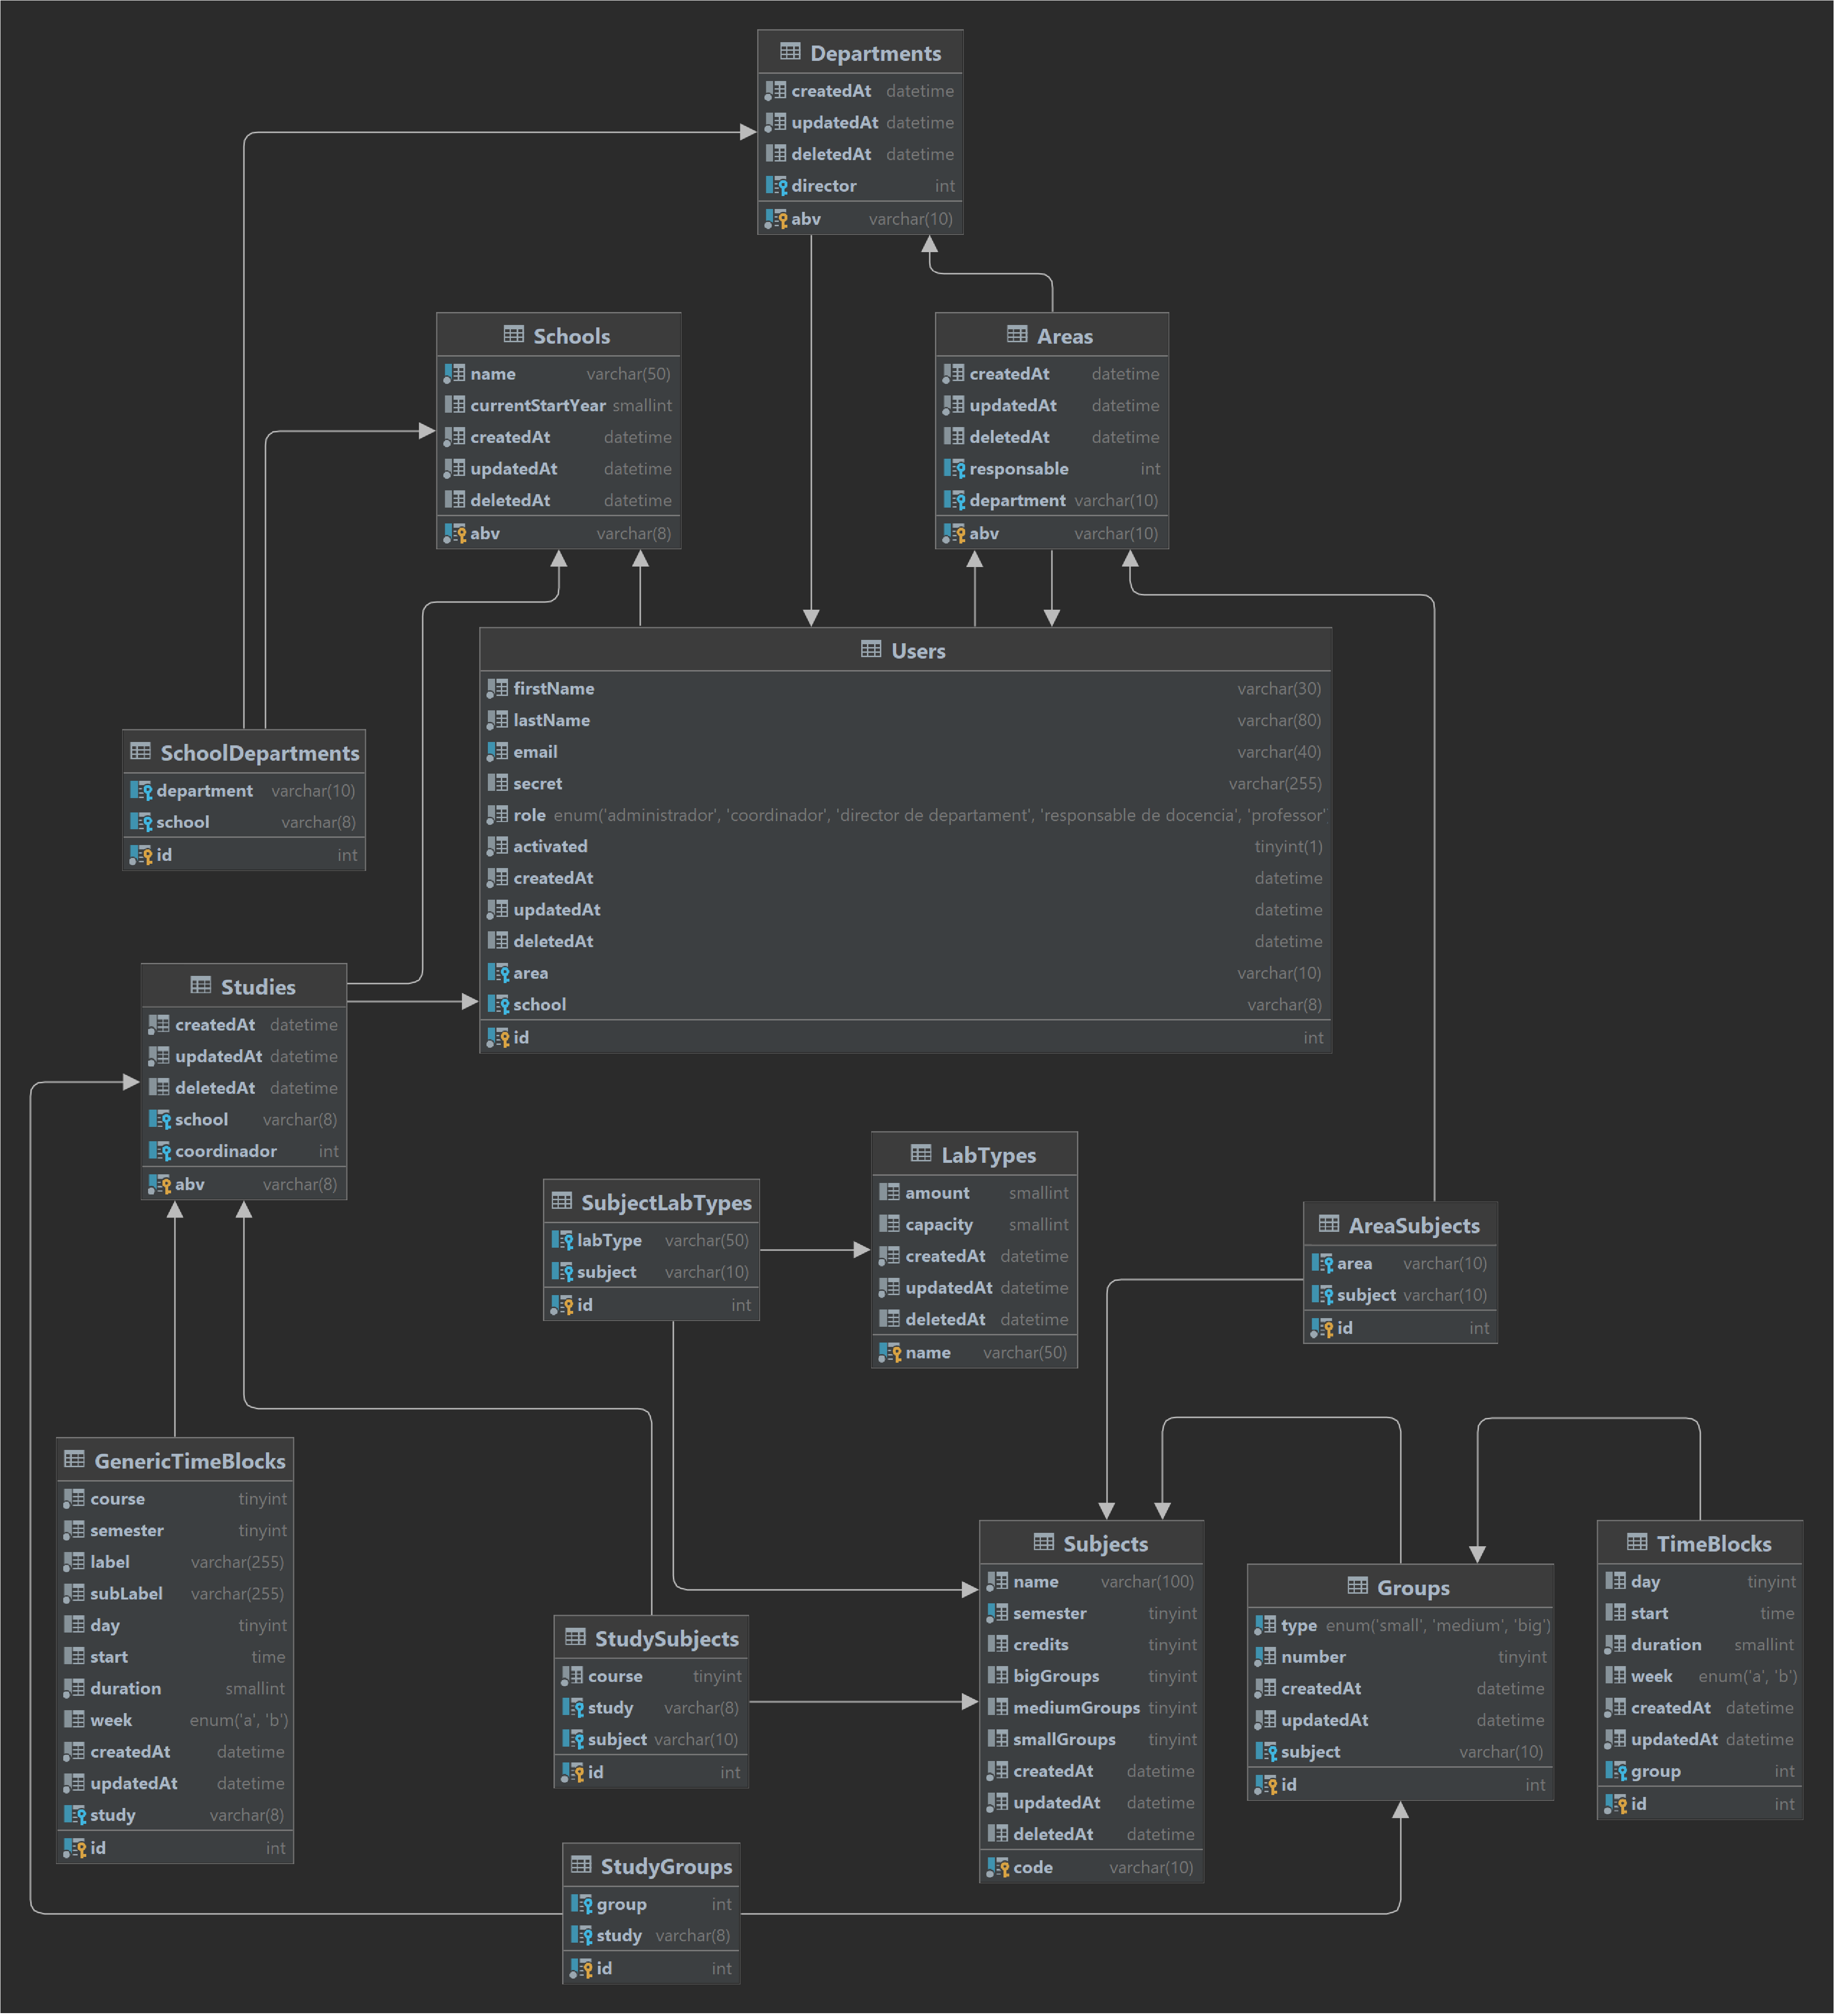
\includegraphics[width=\textwidth]{assets/db.pdf}
	\caption{\label{img:db}Diagrama relacional de la base de dades.}
\end{figure}

\subsection{Descripció de les entitats}
\label{subsec:bd_entitats}

\subsubsection{Consideracions inicials}

En aquest apartat, es presentaran una sèrie de consideracions inicials amb l'objectiu de clarificar el contingut dels que segueixen.

En primer lloc, és necessari definir el format que adoptarà cadascun dels atributs de les taules:
\\[8pt]
\centerline{\texttt{\textbf{Nom} <Tipus> [Restriccions]}: Descripció}

D'altra banda, cal destacar que la majoria de les taules disposen de tres atributs comuns, els quals només es descriuen a continuació per tal d'evitar repeticions innecessàries:
\begin{itemize}
  \item \texttt{\textbf{createdAt} <datetime> [NOT NULL]}: Moment de la creació de l'entitat.
  \item \texttt{\textbf{updatedAt} <datetime> [NOT NULL]}: Moment de l'última modificació de l'entitat.
  \item \texttt{\textbf{deletedAt} <datetime>}: Moment de l'eliminació de l'entitat.
\end{itemize}

\subsubsection{Facultats o \textit{Schools}}

En aquest apartat, es descriuran els atributs de la taula ``Facultats'' (``\textit{Schools}'' al diagrama):
\begin{itemize}
  \item \texttt{\textbf{abv} <varchar(8)> [PRIMARY KEY]}: Abreviació (clau primària).
  \item \texttt{\textbf{name} <varchar(50)> [NOT NULL]}: Nom.
  \item \texttt{\textbf{currentStartYear} <smallint>}: Any d'inici del curs acadèmic actual.
\end{itemize}

\subsubsection{Usuaris o \textit{Users}}

En aquest apartat, es descriuran els atributs de la taula ``Usuaris'' (``\textit{Users}'' al diagrama):
\begin{itemize}
  \item \texttt{\textbf{id} <int> [PRIMARY KEY AUTOINCREMENT]}: Identificador numèric (clau primària).
  \item \texttt{\textbf{firstName} <varchar(30)> [NOT NULL]}: Nom.
  \item \texttt{\textbf{lastName} <varchar(80)> [NOT NULL]}: Cognoms.
  \item \texttt{\textbf{email} <varchar(40)> [NOT NULL]}: Adreça de correu electrònic.
  \item \texttt{\textbf{secret} <varchar(255)> [NOT NULL]}: Contrasenya (encriptada).
  \item \texttt{\textbf{role} <ENUM(<llista de rols>)> [NOT NULL]}: Rol.
  \item \texttt{\textbf{activated} <tinyint(1)> [DEFAULT 0]}: Indica si l'usuari ha estat activat o no.
  \item \texttt{\textbf{area} <varchar(10)>}: En cas que el rol sigui Professor, abreviació de l'àrea a la qual pertany (clau forana).
  \item \texttt{\textbf{school} <varchar(8)>}: Abreviació de la facultat a la qual pertany (clau forana).
\end{itemize}

\subsubsection{Departaments o \textit{Departments}}

En aquest apartat, es descriuran els atributs de la taula ``Departaments'' (``\textit{Departments}'' al diagrama):
\begin{itemize}
  \item \texttt{\textbf{abv} <varchar(10)> [PRIMARY KEY]}: Abreviació (clau primària).
  \item \texttt{\textbf{director} <int>}: Identificador numèric de l'usuari que el dirigeix (clau forana).
\end{itemize}

\subsubsection{FacultatDepartaments o \textit{SchoolDepartments}}

En aquest apartat, es descriuran els atributs de la taula ``FacultatDepartaments'' (``\textit{SchoolDepartments}'' al diagrama):
\begin{itemize}
  \item \texttt{\textbf{id} <int> [PRIMARY KEY]}: Identificador numèric (clau primària).
  \item \texttt{\textbf{school} <varchar(8)>}: Abreviació de la facultat a la qual pertany (clau forana).
  \item \texttt{\textbf{department} <varchar(10)>}: Abreviació del departament al qual pertany (clau forana).
\end{itemize}

Aquesta taula també conté un índex que assegura la unicitat de la parella d'atributs ``\textit{school}'' - ``\textit{department}''.

\subsubsection{Àrees o \textit{Areas}}

En aquest apartat, es descriuran els atributs de la taula ``Àrees'' (``\textit{Areas}'' al diagrama):
\begin{itemize}
  \item \texttt{\textbf{abv} <varchar(10)> [PRIMARY KEY]}: Abreviació (clau primària).
  \item \texttt{\textbf{responsable} <int>}: Identificador numèric de l'usuari que la gestiona (clau forana).
  \item \texttt{\textbf{departament} <int>}: Abreviació del departament al qual pertany (clau forana).
\end{itemize}

\subsubsection{Estudis o \textit{Studies}}

En aquest apartat, es descriuran els atributs de la taula ``Estudis'' (``\textit{Studies}'' al diagrama):
\begin{itemize}
  \item \texttt{\textbf{abv} <varchar(8)> [PRIMARY KEY]}: Abreviació (clau primària).
  \item \texttt{\textbf{school} <varchar(8)>}: Abreviació de la facultat a la qual pertany (clau forana).
  \item \texttt{\textbf{coordinador} <int>}: Identificador numèric de l'usuari que el gestiona (clau forana).
\end{itemize}

\subsubsection{Assignatures o \textit{Subjects}}

En aquest apartat, es descriuran els atributs de la taula ``Assignatures'' (``\textit{Subjects}'' al diagrama):
\begin{itemize}
  \item \texttt{\textbf{code} <varchar(10)> [PRIMARY KEY]}: Codi (clau primària).
  \item \texttt{\textbf{name} <varchar(100)> [NOT NULL]}: Nom.
  \item \texttt{\textbf{semester} <tinyint> [NOT NULL]}: Semestre durant el qual es cursa.
  \item \texttt{\textbf{credits} <tinyint>}: Nombre de crèdits.
  \item \texttt{\textbf{bigGroups} <tinyint>}: Nombre de grups grans que ha de tenir.
  \item \texttt{\textbf{mediumGroups} <tinyint>}: Nombre de grups mitjans que ha de tenir.
  \item \texttt{\textbf{smallGroups} <tinyint>}: Nombre de grups petits que ha de tenir.
\end{itemize}

\subsubsection{EstudiAssignatures o \textit{StudySubjects}}

En aquest apartat, es descriuran els atributs de la taula ``EstudiAssignatures'' (``\textit{StudySubjects}'' al diagrama):
\begin{itemize}
  \item \texttt{\textbf{id} <int> [PRIMARY KEY]}: Identificador numèric (clau primària).
  \item \texttt{\textbf{course} <tinyint> [NOT NULL]}: Curs en el qual es cursa l'assignatura a l'estudi.
  \item \texttt{\textbf{study} <varchar(8)>}: Abreviació de l'estudi al qual pertany (clau forana).
  \item \texttt{\textbf{subject} <varchar(10)>}: Codi de l'assignatura a la qual pertany (clau forana).
\end{itemize}

Aquesta taula també conté un índex que assegura la unicitat de la parella d'atributs ``\textit{study}'' - ``\textit{subject}''.

\subsubsection{ÀreaAssignatures o \textit{AreaSubjects}}

En aquest apartat, es descriuran els atributs de la taula ``ÀreaAssignatures'' (``\textit{AreaSubjects}'' al diagrama):
\begin{itemize}
  \item \texttt{\textbf{id} <int> [PRIMARY KEY]}: Identificador numèric (clau primària).
  \item \texttt{\textbf{area} <varchar(10)>}: Abreviació de l'àrea a la qual pertany (clau forana).
  \item \texttt{\textbf{subject} <varchar(10)>}: Codi de l'assignatura a la qual pertany (clau forana).
\end{itemize}

Aquesta taula també conté un índex que assegura la unicitat de la parella d'atributs ``\textit{area}'' - ``\textit{subject}''.

\subsubsection{TipusLaboratori o \textit{LabTypes}}

En aquest apartat, es descriuran els atributs de la taula ``TipusLaboratori'' (``\textit{LabTypes}'' al diagrama):
\begin{itemize}
  \item \texttt{\textbf{name} <varchar(50)> [PRIMARY KEY]}: Nom.
  \item \texttt{\textbf{amount} <smallint>}: Quantitat existent.
  \item \texttt{\textbf{capacity} <smallint>}: Capacitat d'alumnes.
\end{itemize}

\subsubsection{AssignaturaTipusLaboratori o \textit{SubjectLabTypes}}

En aquest apartat, es descriuran els atributs de la taula ``AssignaturaTipusLaboratori'' (``\textit{SubjectLabTypes}'' al diagrama):
\begin{itemize}
  \item \texttt{\textbf{id} <int> [PRIMARY KEY]}: Identificador numèric (clau primària).
  \item \texttt{\textbf{labType} <varchar(50)>}: Nom del tipus de laboratori al qual pertany (clau forana).
  \item \texttt{\textbf{subject} <varchar(10)>}: Codi de l'assignatura a la qual pertany (clau forana).
\end{itemize}

Aquesta taula també conté un índex que assegura la unicitat de la parella d'atributs ``\textit{labType}'' - ``\textit{subject}''.

\subsubsection{Grups o \textit{Groups}}

En aquest apartat, es descriuran els atributs de la taula ``Grups'' (``\textit{Groups}'' al diagrama):
\begin{itemize}
  \item \texttt{\textbf{id} <int> [PRIMARY KEY]}: Identificador numèric (clau primària).
  \item \texttt{\textbf{type} <enum(`small', `medium', `big')> [NOT NULL]}: Tipus.
  \item \texttt{\textbf{number} <tinyint> [NOT NULL]}: Número (numeració segons tipus).
  \item \texttt{\textbf{subject} <varchar(10)>}: Codi de l'assignatura a la qual pertany (clau forana).
\end{itemize}

\subsubsection{EstudiGrups o \textit{StudyGroups}}

En aquest apartat, es descriuran els atributs de la taula ``EstudiGrups'' (``\textit{StudyGroups}'' al diagrama):
\begin{itemize}
  \item \texttt{\textbf{id} <int> [PRIMARY KEY]}: Identificador numèric (clau primària).
  \item \texttt{\textbf{group} <int>}: Identificador numèric del grup al qual pertany (clau forana).
  \item \texttt{\textbf{study} <varchar(8)>}: Abreviació de l'estudi al qual pertany (clau forana).
\end{itemize}

Aquesta taula també conté un índex que assegura la unicitat de la parella d'atributs ``\textit{group}'' - ``\textit{study}''.

\subsubsection{BlocsHoraris o \textit{TimeBlocks}}

En aquest apartat, es descriuran els atributs de la taula ``BlocsHoraris'' (``\textit{TimeBlocks}'' al diagrama):
\begin{itemize}
  \item \texttt{\textbf{id} <int> [PRIMARY KEY]}: Identificador numèric (clau primària).
  \item \texttt{\textbf{day} <tinyint>}: Dia de la setmana al qual està assignat.
  \item \texttt{\textbf{start} <time>}: Hora d'inici.
  \item \texttt{\textbf{duration} <smallint> [NOT NULL]}: Duració.
  \item \texttt{\textbf{week} <enum(`A', `B')>}: Setmana a la qual està assignat (NULL si ho està a totes).
  \item \texttt{\textbf{group} <int>}: Identificador numèric del grup al qual pertany (clau forana).
\end{itemize}

\subsubsection{BlocsHorarisGenèrics o \textit{GenericTimeBlocks}}

En aquest apartat, es descriuran els atributs de la taula ``BlocsHorarisGenèrics'' (``\textit{GenericTimeBlocks}'' al diagrama):
\begin{itemize}
  \item \texttt{\textbf{id} <int> [PRIMARY KEY]}: Identificador numèric (clau primària).
  \item \texttt{\textbf{course} <tinyint> [NOT NULL]}: Curs al qual pertany.
  \item \texttt{\textbf{semester} <tinyint> [NOT NULL]}: Semestre al qual pertany.
  \item \texttt{\textbf{label} <varchar(255)> [NOT NULL]}: Etiqueta.
  \item \texttt{\textbf{subLabel} <varchar(255)> [NOT NULL]}: Subetiqueta.
  \item \texttt{\textbf{day} <tinyint>}: Dia de la setmana al qual està assignat.
  \item \texttt{\textbf{start} <time>}: Hora d'inici.
  \item \texttt{\textbf{duration} <smallint> [NOT NULL]}: Duració.
  \item \texttt{\textbf{week} <enum(`A', `B')>}: Setmana a la qual està assignat (NULL si ho està a totes).
  \item \texttt{\textbf{study} <varchar(8)>}: Abreviació de l'estudi al qual està assignat (clau forana).
\end{itemize}

\section{Interfícies d'usuari}
\label{sec:interficies_usuari}

En aquesta secció, s'exposarà el disseny de les diferents finestres que conformaran l'aplicació web client.

Cal destacar que l'aparença final de l'aplicació no ha de ser necessàriament igual que la que es mostrarà a les subseccions següents.

\subsection{Interfícies d'autenticació}
\label{subsec:interficies_auth}

En aquesta subsecció, es presentarà el disseny de les finestres més importants relacionades amb la part de l'autenticació.

A la figura~\ref{img:login} es pot veure el disseny de la finestra en la qual un usuari pot autenticar-se o bé indicar que ha oblidat la seva contrasenya.
\begin{figure}[H]
	\centering
	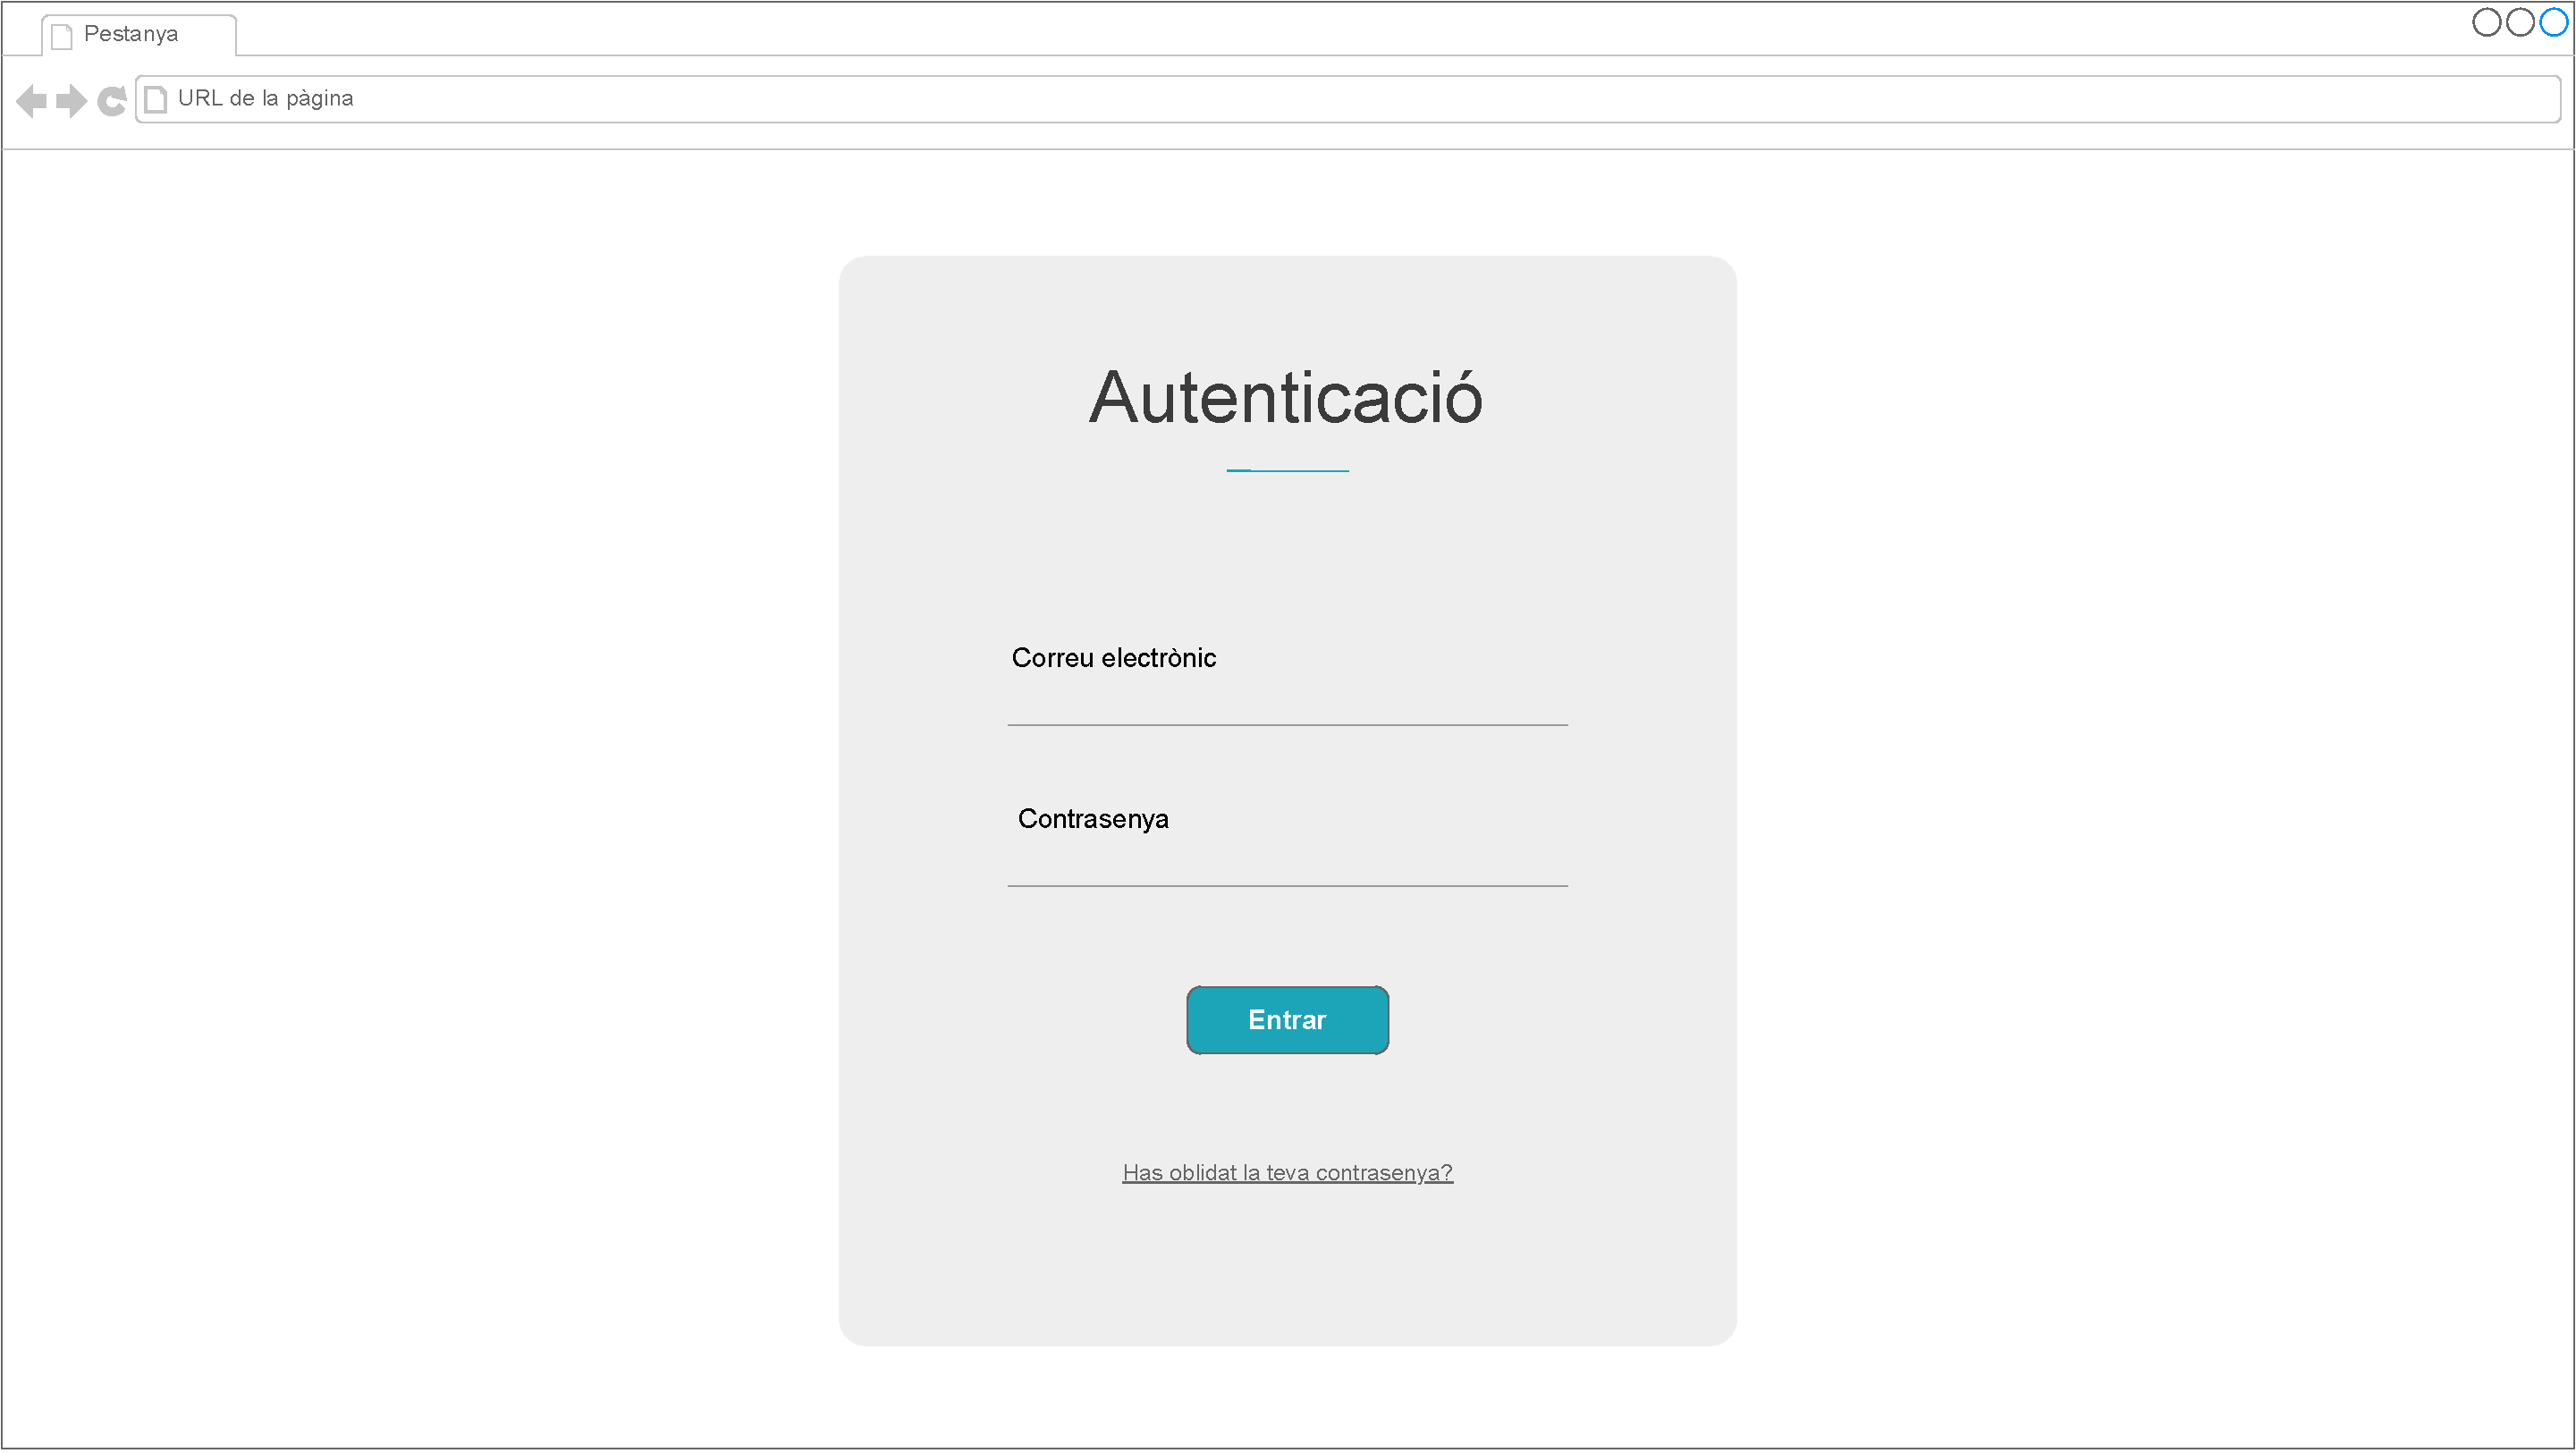
\includegraphics[width=\textwidth]{assets/interfaces/auth/login.pdf}
	\caption{\label{img:login}Disseny de la interfície d'autenticació.}
\end{figure}

A la figura~\ref{img:passwordRestablishment} es pot veure el disseny de la finestra en la qual un usuari pot introduir la seva adreça de correu electrònic per tal de restablir la seva contrasenya o bé tornar a la finestra d'autenticació.
\begin{figure}[H]
	\centering
	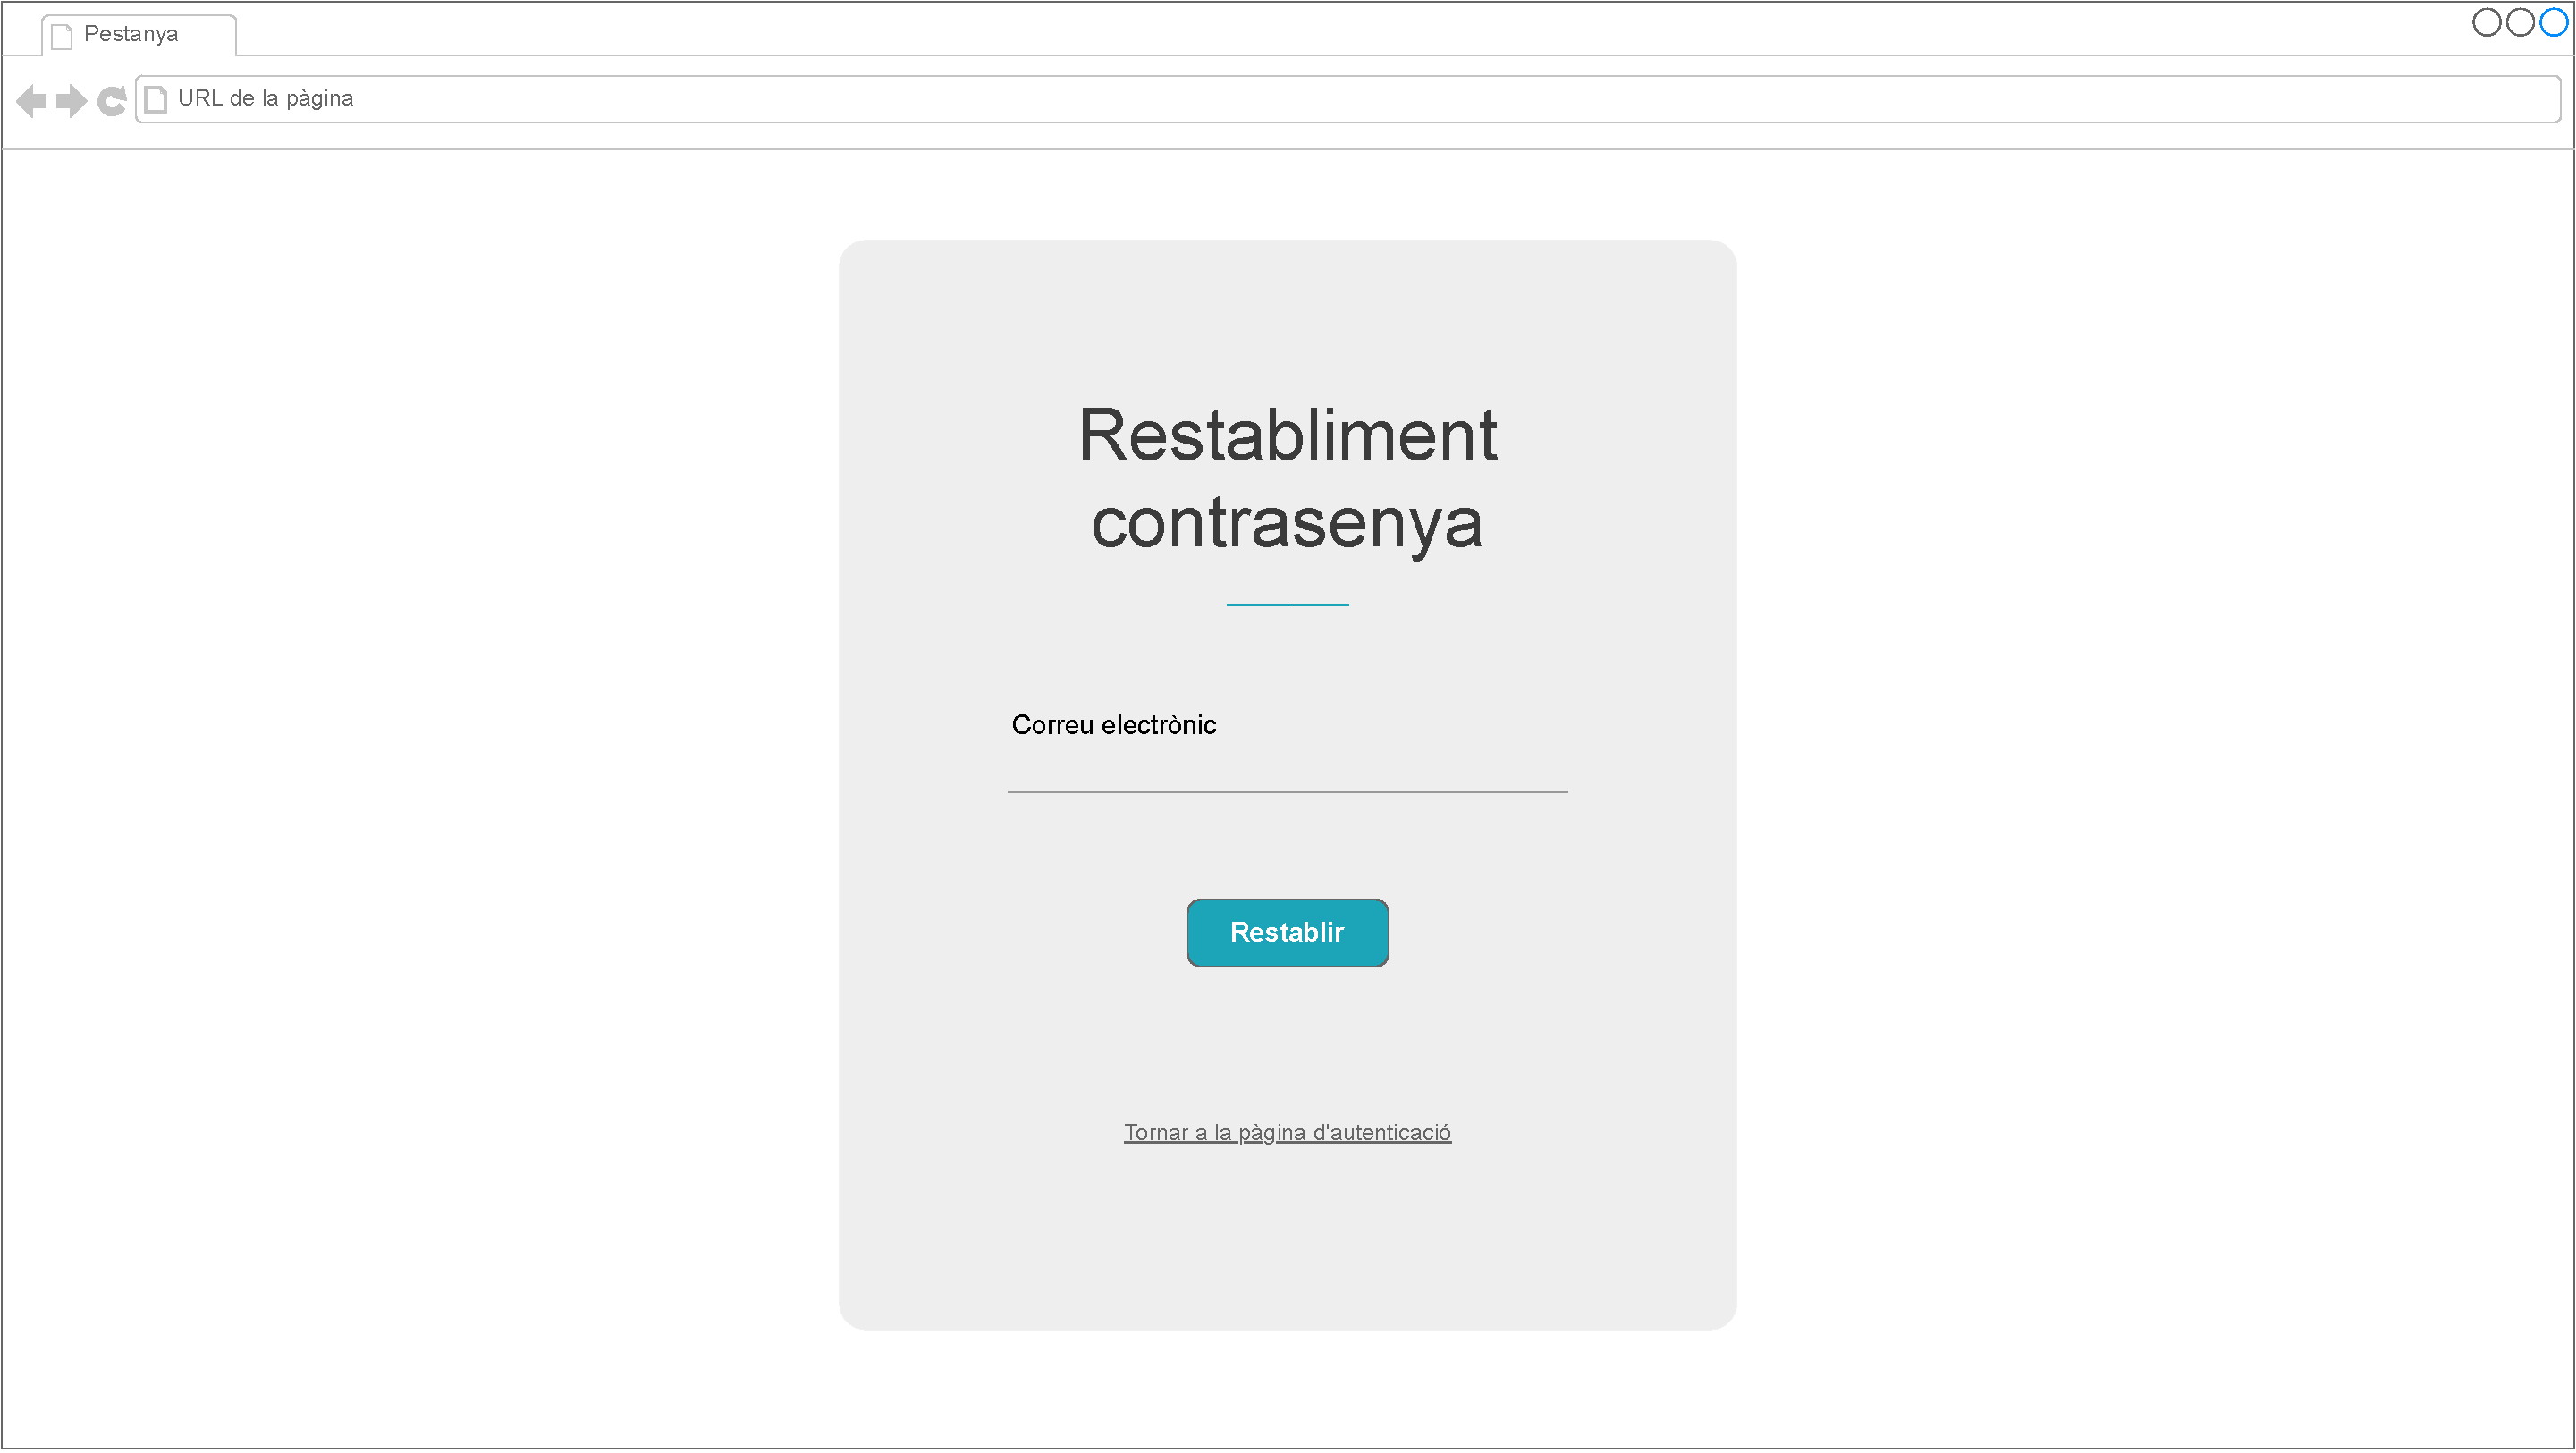
\includegraphics[width=\textwidth]{assets/interfaces/auth/passwordRestablishment.pdf}
	\caption{\label{img:passwordRestablishment}Disseny de la interfície de restabliment de contrasenya.}
\end{figure}

\newpage

A la figura~\ref{img:passwordRestablished} es pot veure el disseny de la finestra en la qual s'informa l'usuari que se li ha enviat un correu electrònic per restablir la seva contrasenya.
\begin{figure}[H]
	\centering
	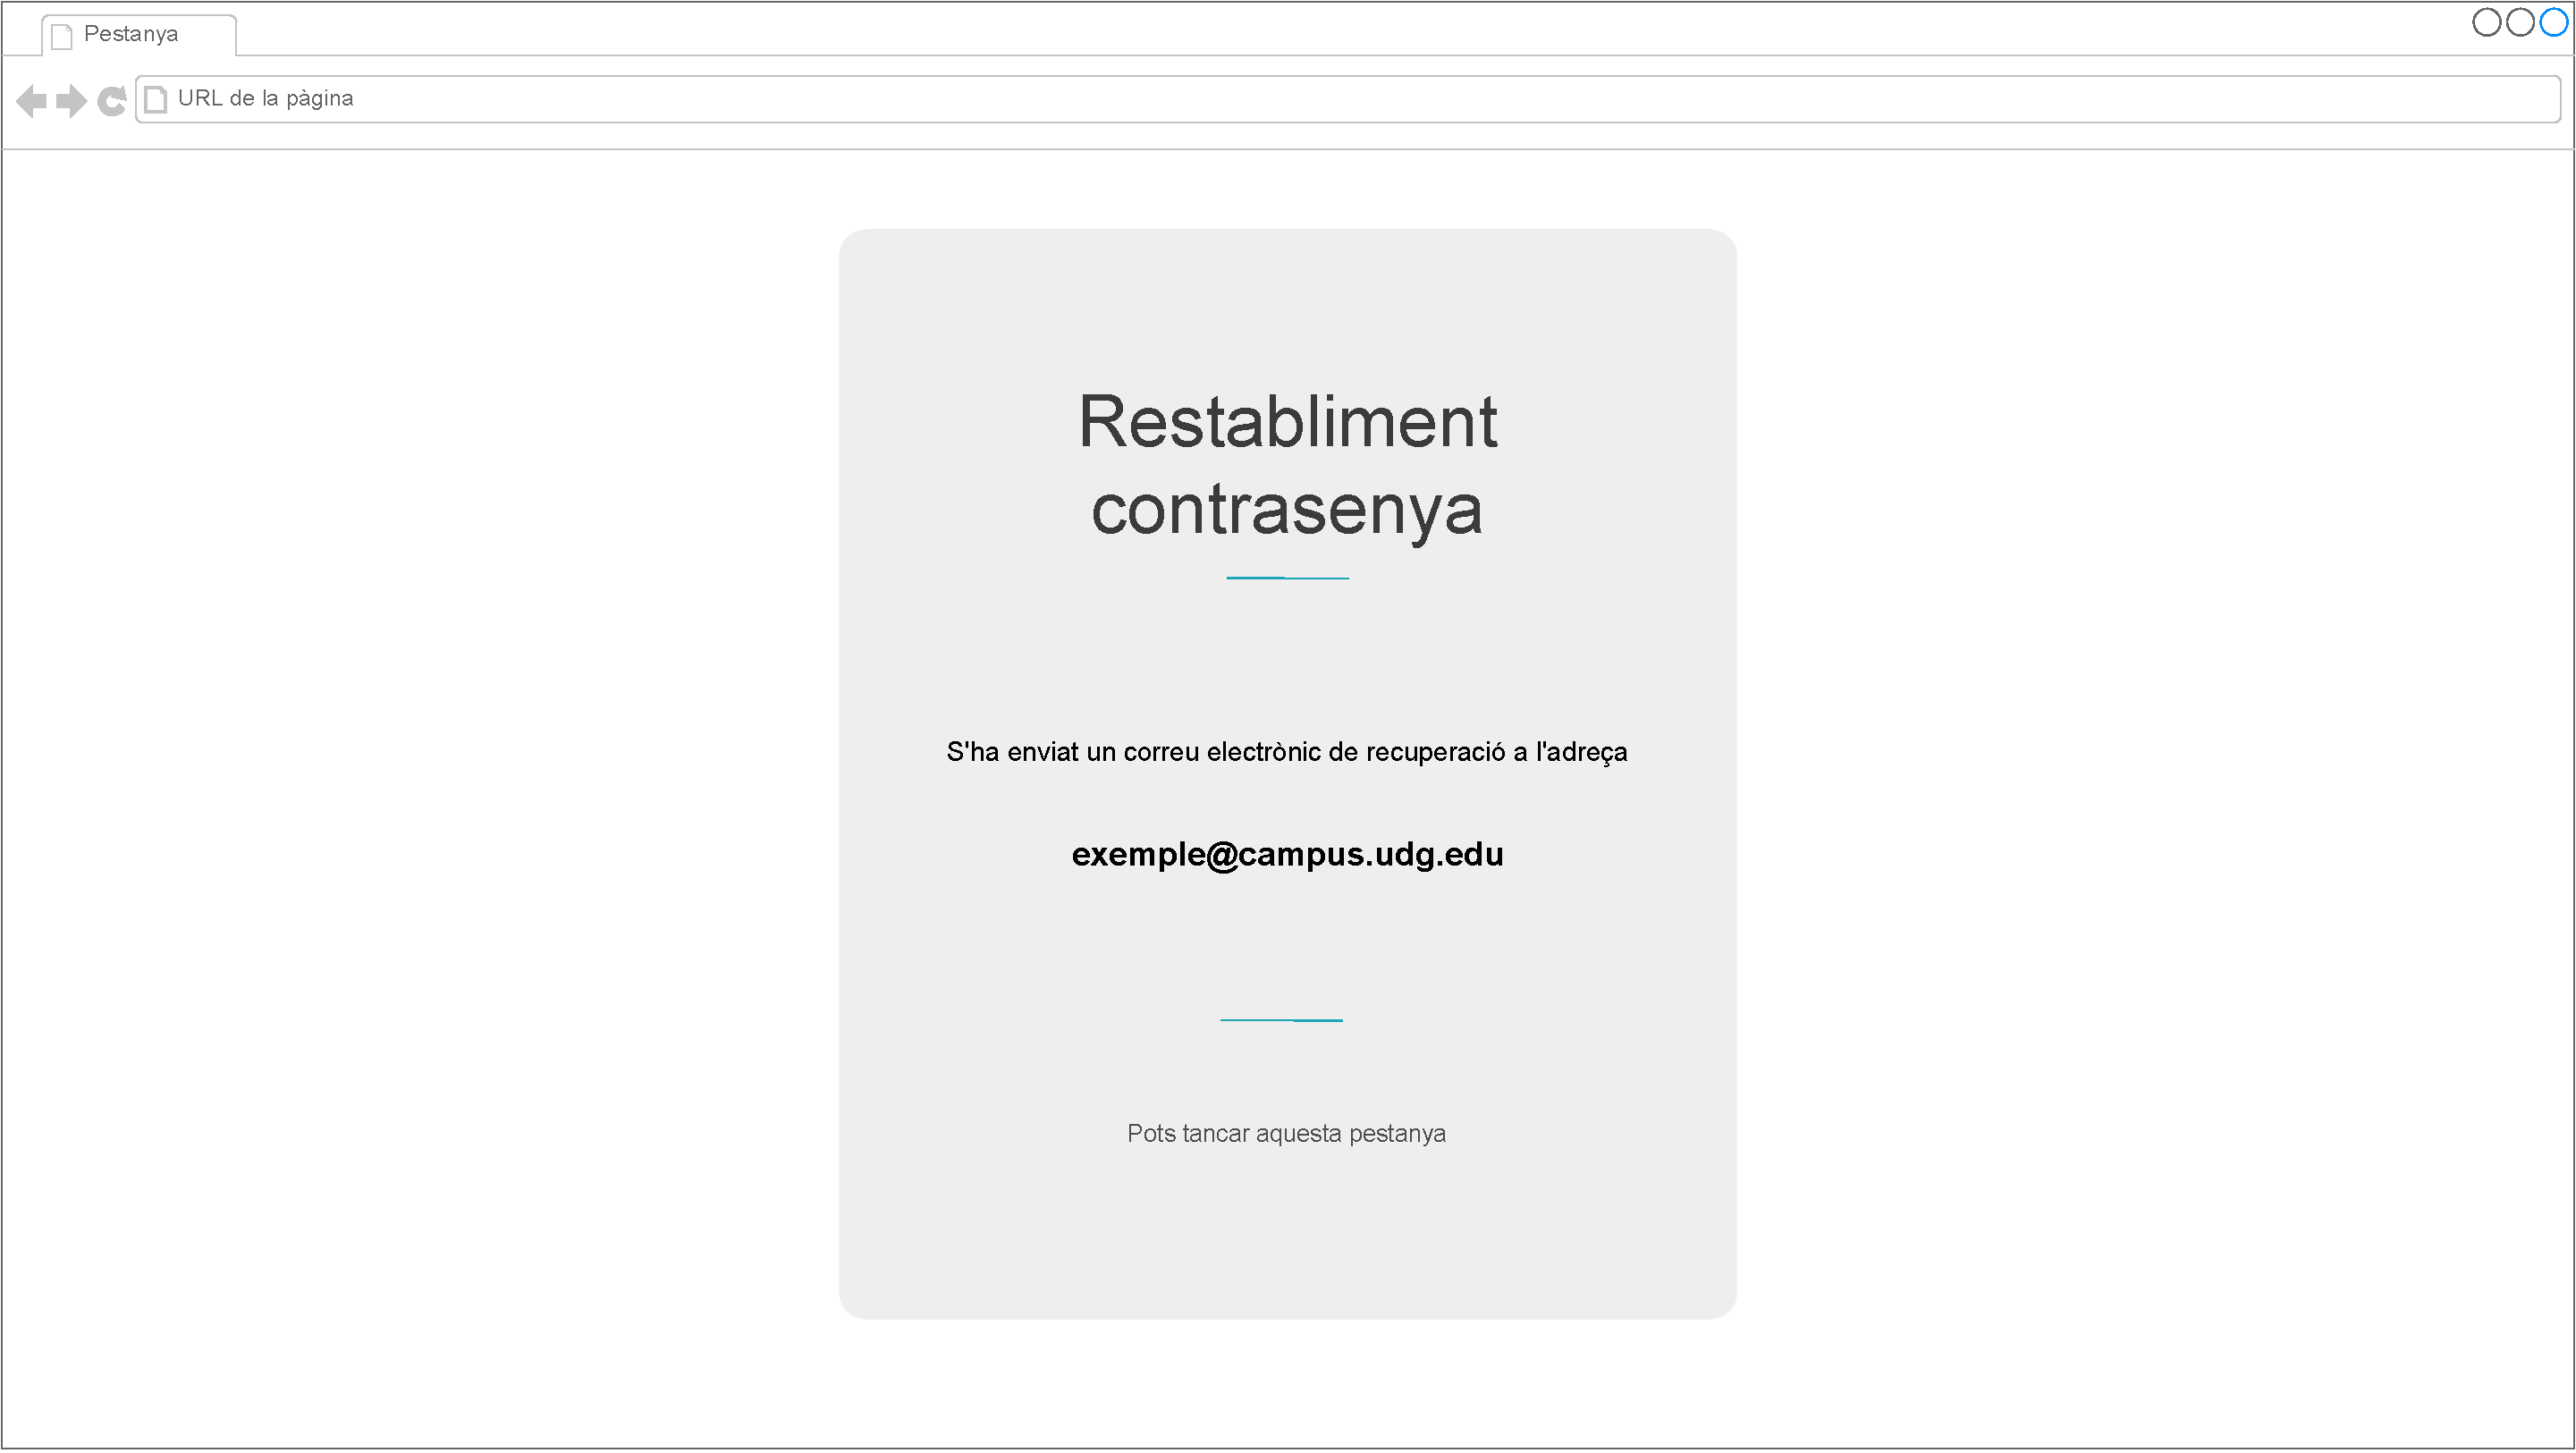
\includegraphics[width=\textwidth]{assets/interfaces/auth/passwordRestablished.pdf}
	\caption{\label{img:passwordRestablished}Disseny de la interfície de confirmació d'enviament d'un \textit{email} per al restabliment de la contrasenya.}
\end{figure}

A la figura~\ref{img:newPassword} es pot veure el disseny de la finestra en la qual l'usuari pot escollir una nova contrasenya.
\begin{figure}[H]
	\centering
	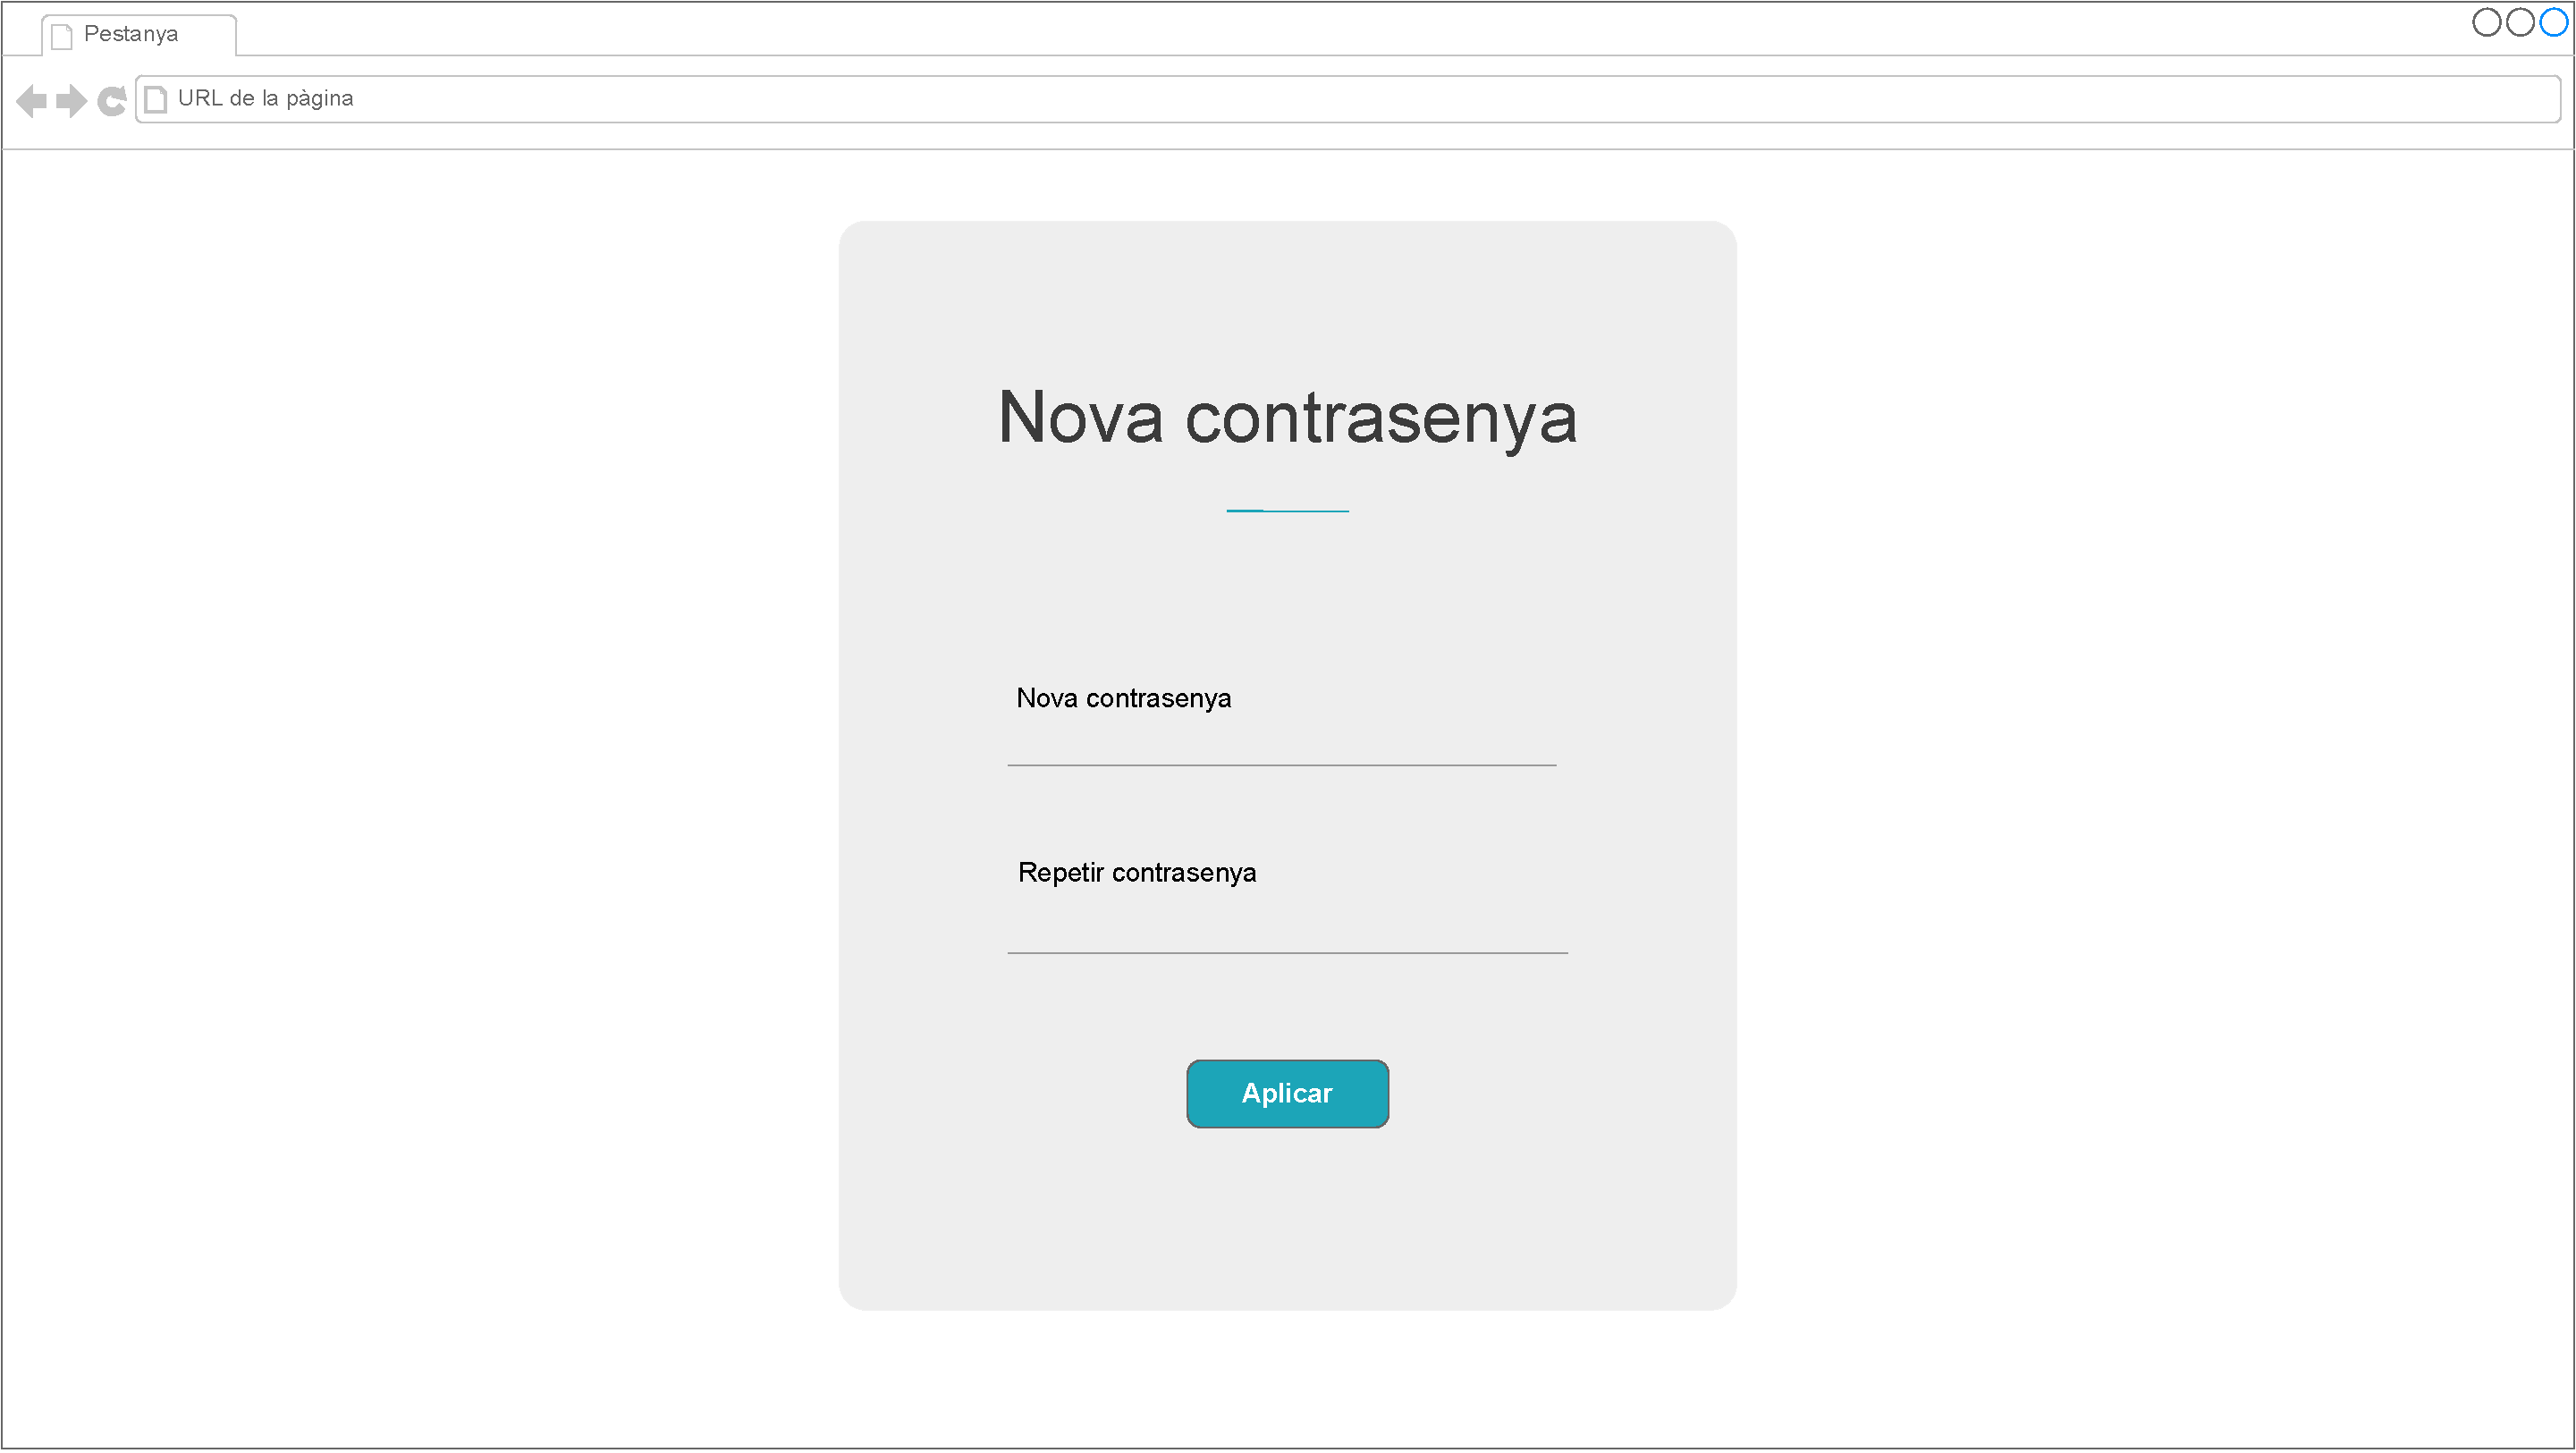
\includegraphics[width=\textwidth]{assets/interfaces/auth/newPassword.pdf}
	\caption{\label{img:newPassword}Disseny de la interfície d'el·lecció d'una nova contrasenya.}
\end{figure}

\subsection{Interfícies de gestió del pla docent}
\label{subsec:interficies_plaDocent}

En aquesta subsecció, es presentarà el disseny de les finestres més importants involucrades en la gestió del pla docent.

A la figura~\ref{img:plaDocent_pujada} es pot veure el disseny de la finestra en la qual un Administrador pot pujar el fitxer d'un pla docent per a la seva facultat i iniciar així el següent curs acadèmic. 

\begin{figure}[H]
	\centering
	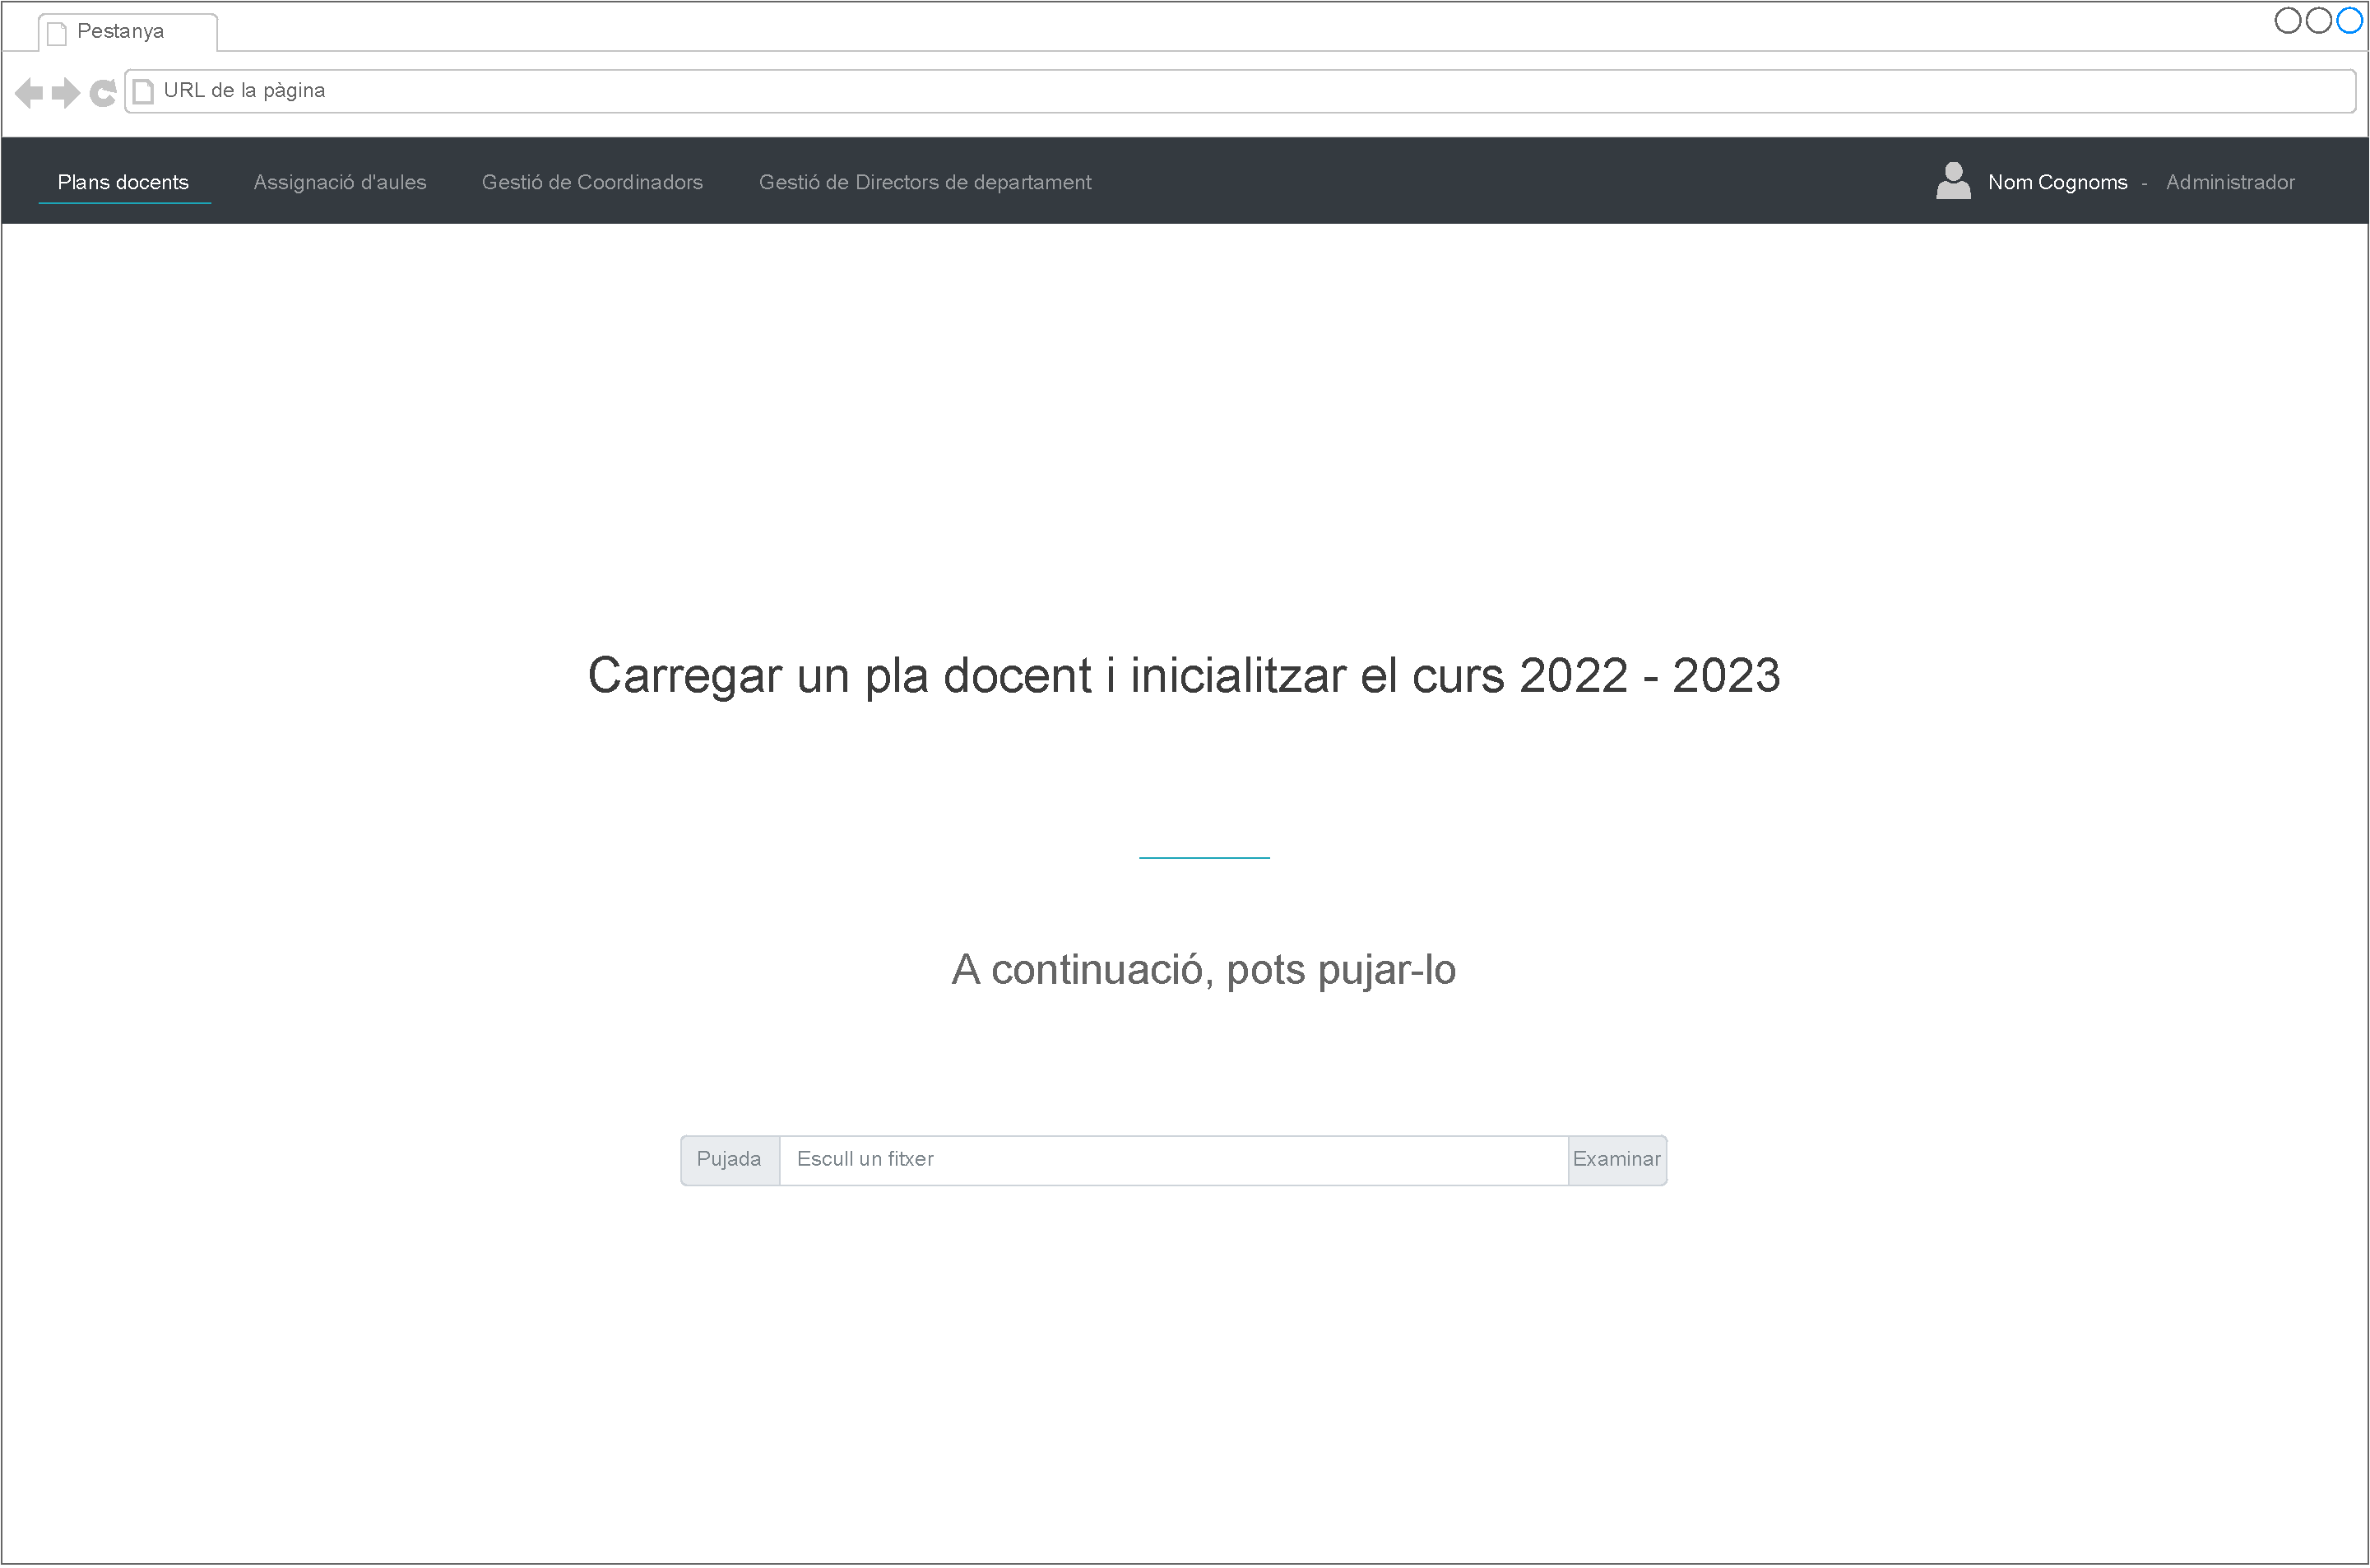
\includegraphics[width=\textwidth]{assets/interfaces/plaDocent/pujada.pdf}
	\caption{\label{img:plaDocent_pujada}Disseny de la interfície de la pujada d'un pla docent.}
\end{figure}

\newpage

A la figura~\ref{img:plaDocent_general} es pot veure el disseny de la finestra en la qual un Administrador pot consultar la informació general del pla docent actual, accedir a la modificació de les dades pertinents o bé anar a la finestra de pujada d'un pla docent per tal d'iniciar el curs següent.

\begin{figure}[H]
	\centering
	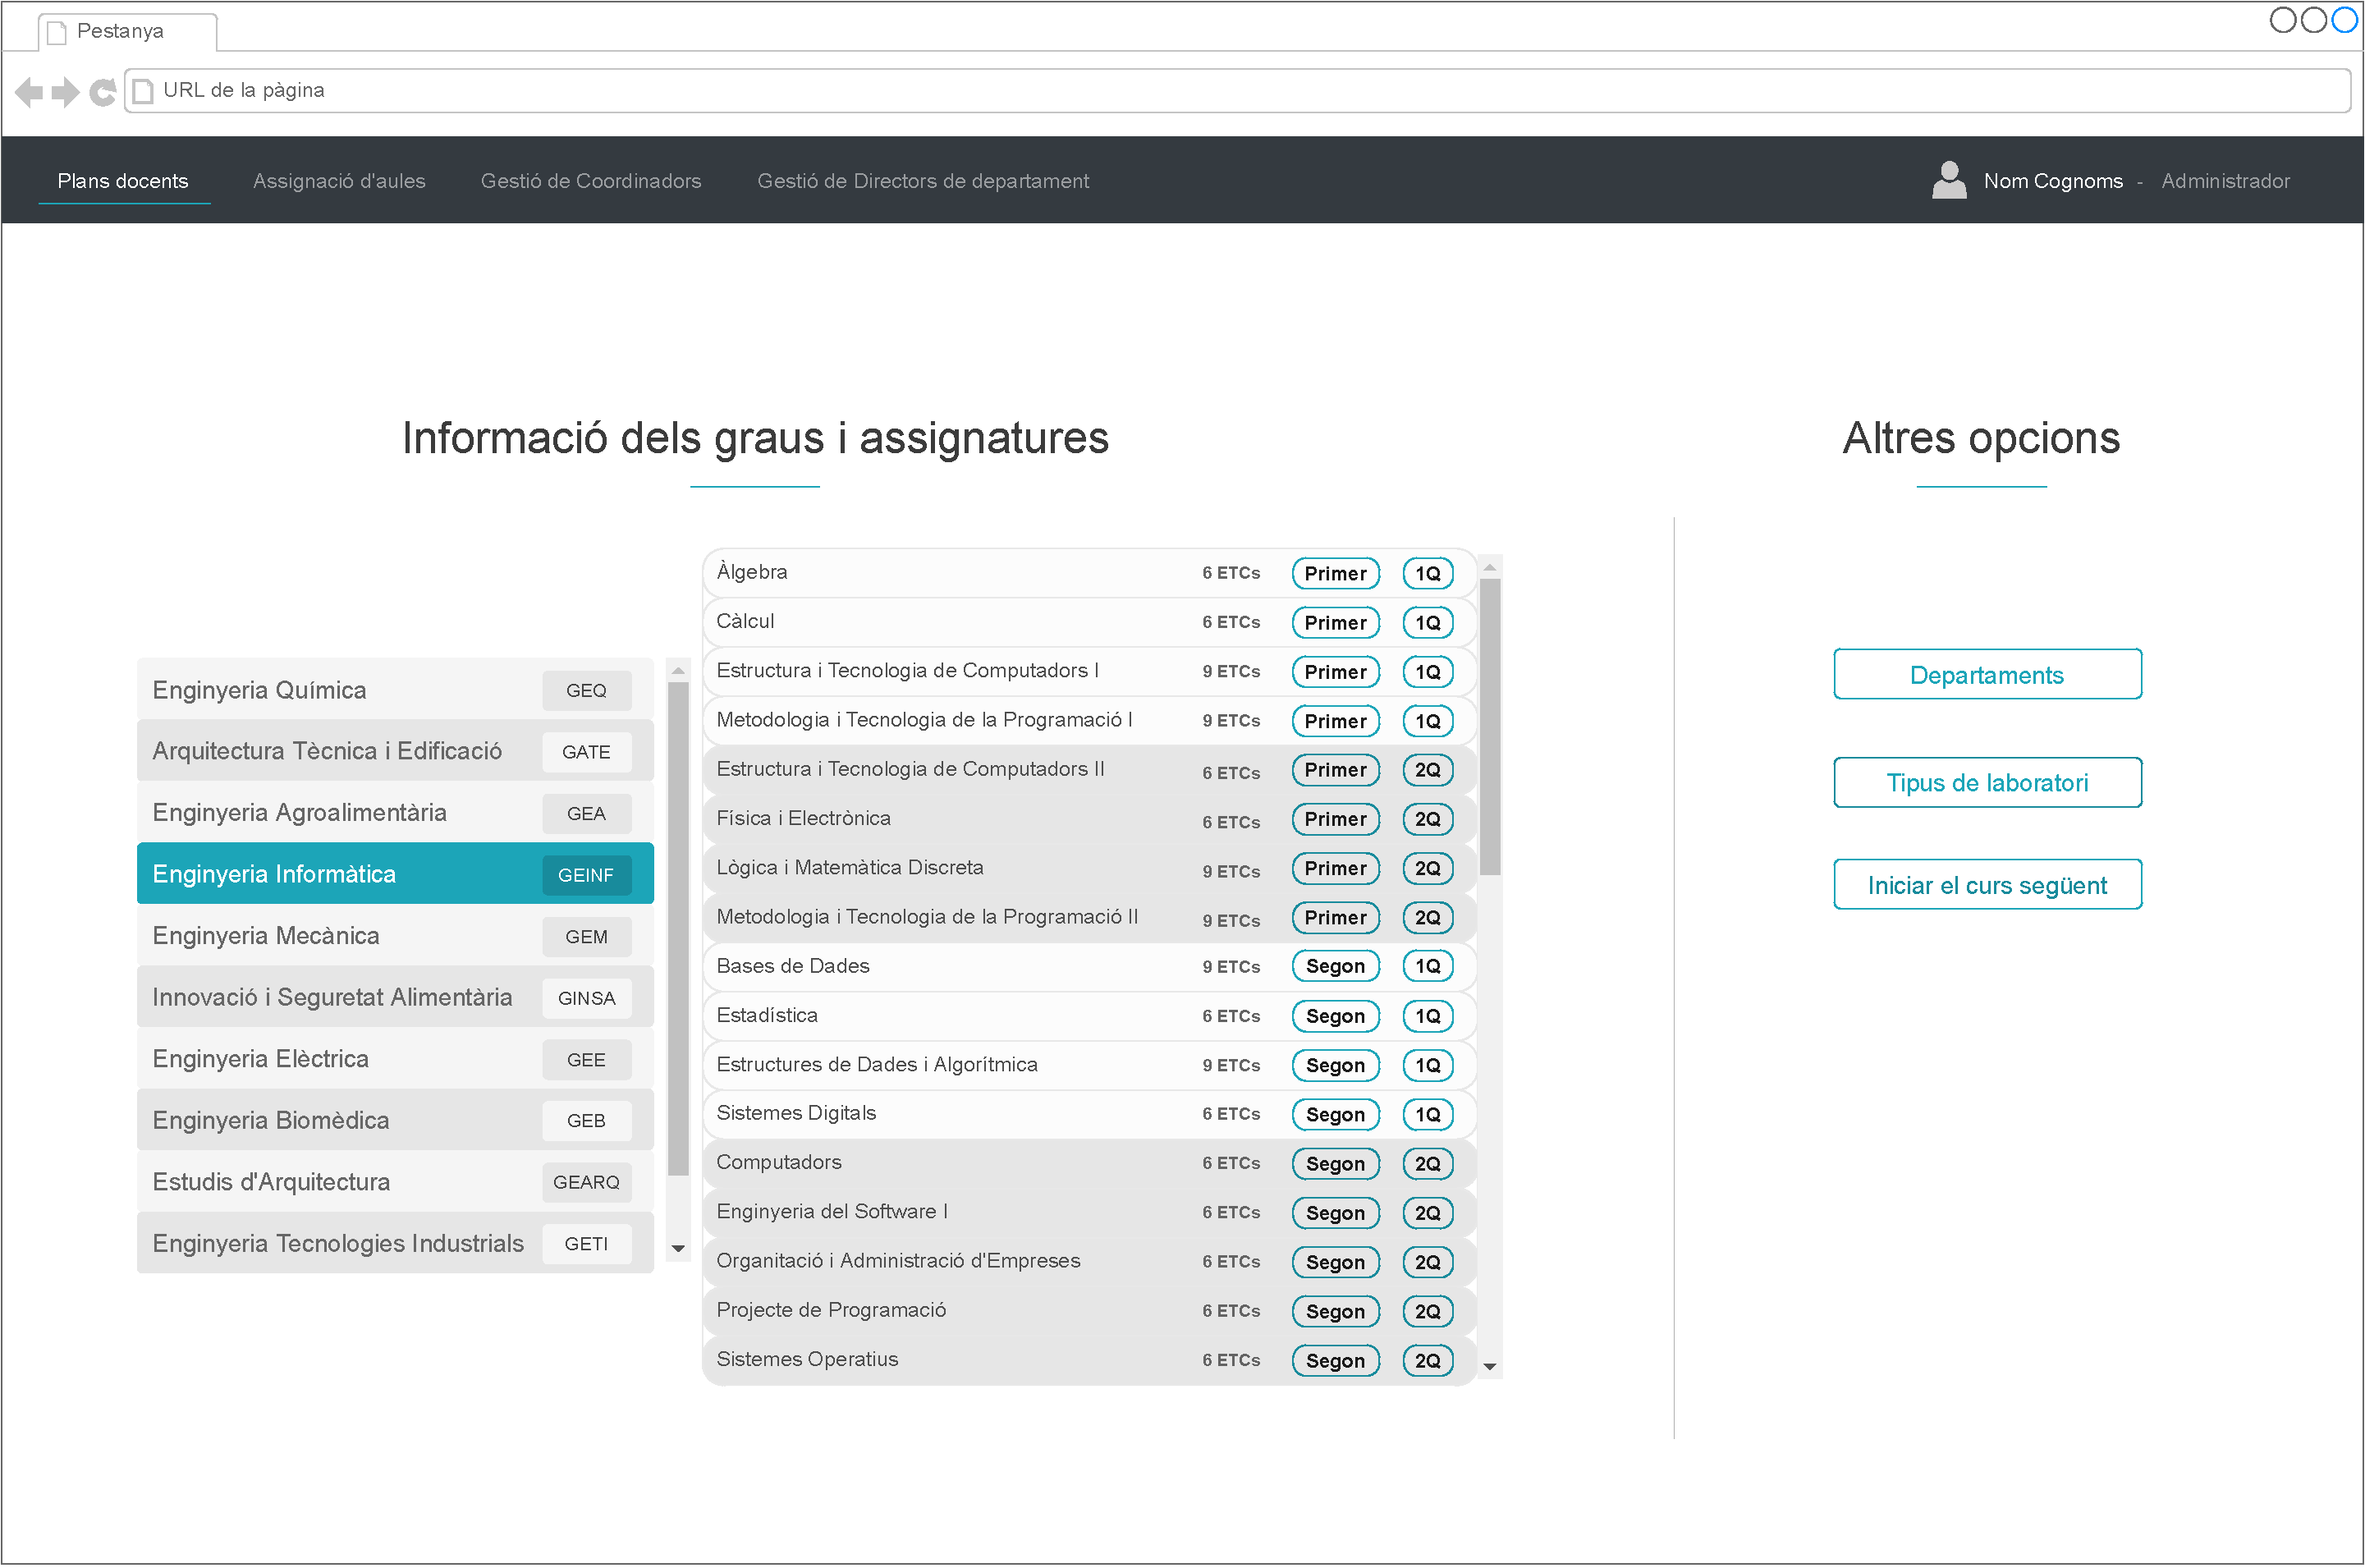
\includegraphics[width=\textwidth]{assets/interfaces/plaDocent/general.pdf}
	\caption{\label{img:plaDocent_general}Disseny de la interfície de gestió del pla docent.}
\end{figure}

\subsection{Interfícies de gestió d'usuaris}
\label{subsec:interficies_gestio_usuaris}

En aquesta subsecció, es presentarà el disseny de les finestres més importants involucrades en la gestió d'usuaris.

Aquests dissenys corresponen a la gestió de Coordinadors i la seva assignació a estudis. No obstant això, també són vàlids per a la gestió de Directors i la seva assignació a departaments, per a la gestió de Responsables de docència i la seva assignació a àrees i per a la gestió de Professors.

A la figura~\ref{img:usuaris_assignacio} es pot veure el disseny de la finestra en la qual un usuari Administrador pot gestionar l'assignació d'usuaris Coordinadors a estudis o bé accedir al seu control.

\begin{figure}[H]
	\centering
	\includegraphics[width=\textwidth]{assets/interfaces/usuaris/assignacio.pdf}
	\caption{\label{img:usuaris_assignacio}Disseny de la interfície d'assignació de Coordinadors a estudis.}
\end{figure}

A la figura~\ref{img:usuaris_assignacio} es pot veure el disseny de la finestra en la qual un usuari Administrador pot controlar usuaris Coordinadors. Més concretament, pot crear-ne, eliminar-ne o bé reenviar el correu electrònic d'activació als que no estiguin activats.
\begin{figure}[H]
	\centering
	\includegraphics[width=\textwidth]{assets/interfaces/usuaris/control.pdf}
	\caption{\label{img:usuaris_control}Disseny de la interfície de control de Coordinadors.}
\end{figure}

A la figura~\ref{img:usuaris_crear} es pot veure el disseny de la finestra en la qual un usuari Administrador pot introduir les dades necessàries per crear nous usuaris Coordinadors.
\begin{figure}[H]
	\centering
	\includegraphics[width=0.4\textwidth]{assets/interfaces/usuaris/crear.pdf}
	\caption{\label{img:usuaris_crear}Disseny de la interfície de creació de Coordinadors.}
\end{figure}

\newpage

\subsection{Interfícies de consulta i elaboració d'horaris}
\label{subsec:interficies_horaris}

En aquesta subsecció, es presentarà el disseny de les finestres més importants involucrades en la consulta i l'elaboració d'horaris.

A la figura~\ref{img:horaris_seleccioEstudi} es pot veure el disseny de la finestra en la qual un usuari Coordinador pot accedir a les finestres de visualització o de modificació d'un horari del grau que gestiona o bé a la selecció d'un horari dels estudis els quals comparteixen alguna assignatura amb el seu per tal de visualitzar-lo.

Aquest disseny també és vàlid per a l'accés a la visualització dels horaris dels estudis corresponents per part d'un Director de departament o d'un Professor.

\begin{figure}[H]
	\centering
	\includegraphics[width=\textwidth]{assets/interfaces/horaris/seleccioEstudi.pdf}
	\caption{\label{img:horaris_seleccioEstudi}Disseny de la interfície d'accés a la gestió d'un horari d'un estudi.}
\end{figure}

\newpage

A la figura~\ref{img:horaris_seleccioProfessor} es pot veure el disseny de la finestra en la qual un usuari Coordinador pot accedir a la visualització d'un horari d'un dels Professors que imparteixen docència al seu grau.

Aquest disseny també és vàlid per a l'accés a la visualització dels horaris dels professors corresponents per part d'un Director de departament o d'un Responsable de docència.

\begin{figure}[H]
	\centering
	\includegraphics[width=\textwidth]{assets/interfaces/horaris/seleccioProfessor.pdf}
	\caption{\label{img:horaris_seleccioProfessor}Disseny de la interfície d'accés a la visualització d'un horari d'un Professor.}
\end{figure}

\newpage

A la figura~\ref{img:horaris_seleccioAula} es pot veure el disseny de la finestra en la qual un usuari Coordinador pot accedir a la visualització d'un horari d'una aula.

\begin{figure}[H]
	\centering
	\includegraphics[width=\textwidth]{assets/interfaces/horaris/seleccioAula.pdf}
	\caption{\label{img:horaris_seleccioAula}Disseny de la interfície d'accés a la visualització d'un horari d'una aula.}
\end{figure}

\newpage

A la figura~\ref{img:horaris_visualitzacio} es pot veure el disseny de la finestra en la qual un usuari Coordinador visualitza un horari d'un estudi. A més a més, pot alternar entre les diferents vistes setmanals, accedir al detall d'un bloc horari i tornar a la finestra de selecció d'horaris.

Aquest disseny també és vàlid per a la visualització d'horaris tant de Professors com d'aules.

Cal destacar que s'ha tingut molt en compte el fet que es pugui visualitzar tota la informació necessària sense haver de fer cap clic, cosa que ha resultat notablement dificultosa a causa de la gran quantitat de dades a distribuïr en un espai bastant limitat.

\begin{figure}[H]
	\centering
	\includegraphics[width=\textwidth]{assets/interfaces/horaris/visualitzacio.pdf}
	\caption{\label{img:horaris_visualitzacio}Disseny de la interfície de visualització d'un horari d'un estudi.}
\end{figure}

\newpage

A la figura~\ref{img:horaris_modif} es pot veure el disseny de la finestra en la qual un usuari Coordinador visualitza un horari d'un estudi i pot realitzar-hi modificacions: pot crear blocs horaris, arrossegar-ne, canviar-ne la mida, la setmana, etc. A més a més, pot accedir al detall d'un bloc horari i modificar-lo des d'allà. Per últim, pot accedir a un menú d'opcions per modificar certes configuracions, com ara habilitar o deshabilitar opcions de filtratge, de visualització de solapaments, etc.

\begin{figure}[H]
  \centering
  \includegraphics[width=\textwidth]{assets/interfaces/horaris/modif.pdf}
  \caption{\label{img:horaris_modif}Disseny de la interfície de modificació d'un horari d'un estudi.}
\end{figure}


\chapter{Implementació i proves}
\label{cap:implementacio}



% Seguretat, autenticació (incloure: quan usuari desactivat o eliminat), ruta dels horaris, middlewares i utilitats backend, format de l'API, variables d'entorn, config, enviament de correu, axios i interceptors, stores pinia, detecció solapaments lab?,

% proves de creació de taules, atributs, relacions..., proves a l'API (postman), proves pla docent, proves assignació usuari, proves vistes setmanals horari (i intentar entrar a un que no pot), modificació d'horaris (moure,resize,assignar a estudis, solapaments, filtratge)


\chapter{Implantació i resultats}
\label{cap:implantacio}

\section{Implantació en l'entorn local}
\label{sec:implantacio}

En aquesta secció, es parlarà sobre com l'aplicació del projecte està implantada localment, tant el \textit{front-end} i el \textit{back-end} com el sistema gestor de bases de dades.

L'aplicació de \textit{front-end} és operada pel servidor de desenvolupament que proporciona Vite (veure capítol~\ref{cap:estudi}). Aquest servidor està exposat al domini ``localhost'' i al port TCP 3000 de l'ordinador. Per tal que Vite serveixi l'aplicació, només cal accedir a l'adreça ``http://localhost:3000'' a través del navegador.

Al mateix temps, és necessari que l'aplicació de \textit{back-end} també s'estigui executant i que pugui servir a les peticions que li faci el client. Aquesta aplicació utilitza Node.js (veure capítol~\ref{cap:estudi}) per muntar un servidor que exposa l'API a l'adreça ``http://localhost:8000/api''. L'aplicació client coneix aquesta adreça i és capaç de llançar-hi peticions.

Per últim, el sistema gestor de bases de dades també ha d'estar exposat a la xarxa local per tal que l'aplicació de \textit{back-end} pugui comunicar-s'hi. Tal com s'ha vist al capítol~\ref{cap:estudi}, MySQL s'executa dins d'un contenidor de Docker, el qual n'exposa la connexió a través del port TCP 3306.

A continuació, es repassaran els passos que cal seguir per posar en marxa localment tot el conjunt de l'aplicatiu.
\begin{enumerate}
  \item Instal·lar Docker~\cite{Docker}.
  \item Obrir una terminal i descarregar una imatge de la versió més recent de MySQL:\\
    \centerline{\texttt{> docker pull mysql:latest}}
  \item Aixecar un contenidor amb la imatge descarregada:\\
    \centerline{\texttt{> docker run ---name=<nom contenidor> -p 3306:3306}}
    \centerline{\texttt{--e MYSQL\_ROOT\_PASSWORD=<contrasenya> -d mysql:latest}}
  \item Obrir una terminal dins del contenidor:\\
    \centerline{\texttt{> docker exec -it <nom contenidor> bash}}
  \item Executar-hi MySql i entrar la contrasenya escollida anteriorment:\\
    \centerline{\texttt{> mysql -u root -p}}
  \item Crear-hi l'usuari que farà servir l'aplicació de \textit{back-end}:\\
    \centerline{\texttt{> CREATE USER 'pfg-app-server'@'\%'}}
    \centerline{\texttt{IDENTIFIED BY 'pfg';}}
  \item Proporcionar a l'usuari creat tots els privilegis de la base de dades:\\
    \centerline{\texttt{> GRANT ALL PRIVILEGES ON * . *}}
    \centerline{\texttt{TO 'pfg-app-server'@'\%';}}
  \item Fer efectius els canvis de permisos:\\
    \centerline{\texttt{> FLUSH PRIVILEGES;}}
  \item Crear la base de dades:\\
    \centerline{\texttt{> CREATE SCHEMA pfg\_app\_dev;}}
  \item Clonar el repositori de l'aplicació del projecte en una carpeta local, el qual està disponible a \href{https://github.com/adriribas/pfg-application}{github.com/adriribas/pfg-application}
  \item Definir les variables d'entorn del servidor creant un fitxer anomenat ``.env'' (sense extensió) dins del directori ``/packages/server'' des de l'arrel del projecte que contingui les línies següents:
  \begin{itemize}
    \item \texttt{HOST='localhost'}
    \item \texttt{PORT=8000}
    \item \texttt{DEBUG='pfgs:*'}
    \item \texttt{pfgs\_authJwtPrivateKey='contrasenyaSecreta1'}
    \item \texttt{pfgs\_resetPasswordJwtPrivateKey='contrasenyaSecreta2'}
    \item \texttt{pfgs\_emailConfirmationJwtPrivateKey='contrasenyaSecreta3'}
    \item \texttt{pfgs\_user='pfg-app-server'}
    \item \texttt{pfgs\_dbSecret='pfg'}
  \end{itemize}
  \item Instal·lar la versió 16 de Node.js~\cite{Node}.
  \item Obrir una terminal en el directori arrel de l'aplicació i instal·lar totes les dependències necessàries:\\
    \centerline{\texttt{> npm install}}
  \item Executar l'aplicació de \textit{back-end}:\\
    \centerline{\texttt{> npm run start:server}}
  \item Obrir una altra terminal en el mateix directori i executar l'aplicació de \textit{front-end}:\\
    \centerline{\texttt{> npm run start:client}}
  \item Accedir a \href{http://localhost:3000}{http://localhost:3000} des d'un navegador.
\end{enumerate}

\section{Resultats obtinguts}
\label{sec:resultats}

\subsection{Consideracions inicials}
\label{subsec:resultats_consideracions}

En aquesta subsecció, es presentaran una sèrie de consideracions inicials que cal tenir en compte a la resta de la secció.

Els resultats es presentaran en forma de captures de pantalla que mostren el funcionament del programari desenvolupat durant el projecte. Totes les captures tindran la mateixa mida per tal d'oferir una perspectiva realística de com són les interfícies d'usuari.

A més a més, aquesta secció també fa la funció de manual d'usuari.

És important destacar que, per no sobrecarregar la memòria amb masses imatges, s'han obviat certes parts o estats de les interfícies que no són de vital importància, com ara notificacions d'informació o error, estats de càrrega, seleccionables desplegats, etc.

\newpage

\subsection{Autenticació}
\label{subsec:resultats_auth}

En aquesta subsecció, s'exposaran els resultats obtinguts pel que fa a l'autenticació.

A la figura~\ref{img:resultats_auth_autenticacio} es pot veure la interfície resultant en la qual un usuari pot realitzar les accions següents:
\begin{itemize}
  \item Entrar l'adreça de correu electrònic i contrasenya del seu usuari per tal d'autenticar-se.
  \item Prémer l'enllaç ``Restableix-la aquí'' per tal de procedir a restablir la contrasenya del seu usuari.
\end{itemize}

\begin{figure}[H]
  \centering
  \includegraphics[width=\textwidth]{assets/results/auth/autenticacio.png}
  \caption{\label{img:resultats_auth_autenticacio}Interfíce resultant d'autenticació.}
\end{figure}

\newpage

A la figura~\ref{img:resultats_auth_restabliment} es pot veure la interfície resultant en la qual un usuari pot realitzar, principalment, les accions següents:
\begin{itemize}
  \item Entrar l'adreça de correu electrònic del seu usuari per tal de restablir-ne la contrasenya.
  \item Prémer l'enllaç ``Autentica't aquí'' per tal de procedir a autenticar-se.
\end{itemize}

\begin{figure}[H]
  \centering
  \includegraphics[width=\textwidth]{assets/results/auth/restabliment.png}
  \caption{\label{img:resultats_auth_restabliment}Interfície resultant de restabliment de contrasenya.}
\end{figure}

\newpage

A la figura~\ref{img:resultats_auth_restablerta} es pot veure la interfície resultant en la qual un usuari pot realitzar, principalment, les accions següents:
\begin{itemize}
  \item Informar-se de que se li ha enviat un correu electrònic a través del qual pot restablir la contrasenya del seu usuari.
  \item Prémer l'enllaç ``Fes-ho aquí'' per tal de procedir a autenticar-se.
\end{itemize}

\begin{figure}[H]
  \centering
  \includegraphics[width=\textwidth]{assets/results/auth/restablerta.png}
  \caption{\label{img:resultats_auth_restablerta}Interfície resultant de confirmació d'enviament d'un \textit{email} per al restabliment de la contrasenya.}
\end{figure}

\newpage

A la figura~\ref{img:resultats_auth_novaContrasenya} es pot veure la interfície resultant en la qual un usuari pot realitzar, principalment, l'acció següent:
\begin{itemize}
  \item Entrar dues vegades una contrasenya per tal d'escollir-ne una nova per al seu usuari.
\end{itemize}

\begin{figure}[H]
  \centering
  \includegraphics[width=\textwidth]{assets/results/auth/novaContrasenya.png}
  \caption{\label{img:resultats_auth_novaContrasenya}Interfíce resultant d'el·lecció d'una nova contrasenya.}
\end{figure}

\newpage

A la figura~\ref{img:resultats_auth_logout} es pot veure la interfície resultant en la qual un usuari pot realitzar, principalment, les acció següent:
\begin{itemize}
  \item Prémer el botó ``Sortir'' situat a la part dreta de la barra superior per tal d'obrir un diàleg de confirmació a través del qual pot tancar la sessió.
\end{itemize}

\begin{figure}[H]
  \centering
  \includegraphics[width=\textwidth]{assets/results/auth/logout.png}
  \caption{\label{img:resultats_auth_logout}Interfíce resultant de tancament de sessió.}
\end{figure}

\newpage

\subsection{Gestió del pla docent}
\label{subsec:resultats_plaDocent}

En aquesta subsecció, s'exposaran els resultats obtinguts pel que fa a la gestió del pla docent.

A la figura~\ref{img:resultats_plaDocent_pujada} es pot veure la interfície resultant en la qual un Administrador pot realitzar, principalment, les accions següents:
\begin{itemize}
  \item Seleccionar el fitxer d'un pla docent del seu ordinador per tal de pujar-lo i inicialitzar, d'aquesta manera, el curs acadèmic en qüestió.
\end{itemize}

Cal destacar que es tracta del cas en què encara no s'ha pujat mai cap pla docent al sistema. En la situació d'estar pujant el pla docent del curs acadèmic següent, també es dóna la possibilitat de cancel·lar i tornar a la gestió del pla docent actual.

\begin{figure}[H]
  \centering
  \includegraphics[width=\textwidth]{assets/results/plaDocent/pujada.png}
  \caption{\label{img:resultats_plaDocent_pujada}Interfície resultant de la pujada d'un pla docent.}
\end{figure}

\newpage

A la figura~\ref{img:resultats_plaDocent_estudis} es pot veure la interfície resultant en la qual un Administrador pot realitzar, principalment, les accions següents:
\begin{itemize}
  \item Visualitzar els estudis del pla docent actual.
  \item Prémer un botó de desplegament per tal de visualitzar les assignatures impartides en un curs concret de l'estudi en qüestió.
  \item Alternar entre els cursos de l'estudi en qüestió per tal de visualitzar les assignatures corresponents.
  \item Situar el ratoí sobre l'abreviació d'una àrea o departament d'una assignatura per tal de visualitzar-ne el nom complet.
  \item Prémer el botó de modificació d'una assignatura per tal de procedir a fer-ho.
\end{itemize}

Cal destacar que, igual que passa en les figures~\ref{img:resultats_plaDocent_departaments} i~\ref{img:resultats_plaDocent_tipusLab}, també es possibilita tant alternar entre la informació del pla docent com procedir a iniciar el curs acadèmic següent.

\begin{figure}[H]
  \centering
  \includegraphics[width=\textwidth]{assets/results/plaDocent/estudis.png}
  \caption{\label{img:resultats_plaDocent_estudis} Interfície resultant de visualització i gestió dels estudis i assignatures d'un pla docent.}
\end{figure}

\newpage

A la figura~\ref{img:resultats_plaDocent_modAssignatura} es pot veure la interfície resultant en la qual un Administrador pot realitzar, principalment, les accions següents:
\begin{itemize}
  \item Modificar el nombre de grups de cada tipus de l'assignatura en qüestió.
  \item Desassignar àrees concretes de l'assignatura en qüestió.
  \item Accedir a l'assignació d'una altra àrea.
  \item Situar el ratolí sobre l'abreviació d'un departament per tal de visualitzar-ne el nom complet.
  \item Assignar múltiples tipus de laboratori a l'assignatura en qüestió mitjançant el desplegable.
  \item Desassignar tots els tipus de laboratori de l'assignatura en qüestió.
  \item Desassignar un tipus de laboratori concret de l'assignatura en qüestió.
  \item Prémer el botó ``Guardar'' per tal de fer efectius els canvis.
  \item Prémer el botó ``Cancel·lar'' per tal de descartar els canvis.
\end{itemize}

\begin{figure}[H]
  \centering
  \includegraphics[width=\textwidth]{assets/results/plaDocent/modAssignatura.png}
  \caption{\label{img:resultats_plaDocent_modAssignatura}Interfície resultant de modificació d'una assignatura.}
\end{figure}

\newpage

A la figura~\ref{img:resultats_plaDocent_modAssignaturaArea} es pot veure la interfície resultant en la qual un Administrador pot realitzar, principalment, les accions següents:
\begin{itemize}
  \item Obrir el desplegable ``Departament'' per tal d'escollir el departament que conté l'àrea que vol assignar a l'assignatura en qüestió.
  \item Obrir el desplegable ``Àrea'' per tal d'escollir l'àrea que vol assignar a l'assignatura en qüestió.
\end{itemize}

Cal destacar que el desplegable ``Àrea'' està bloquejat mentre no es selecciona un departament. A més a més, aquest desplegable no conté àrees que ja estan assignades a l'assignatura en qüestió i, en cas que només n'hi hagi una, es selecciona automàticament després d'haver escollit el departament. El botó ``Afegir'' també romandrà bloquejat mentre no s'hagi escollit una àrea concreta.

\begin{figure}[H]
  \centering
  \includegraphics[width=\textwidth]{assets/results/plaDocent/modAssignaturaArea.png}
  \caption{\label{img:resultats_plaDocent_modAssignaturaArea}Interfície resultant de selecció d'una àrea per assignar-la a una assignatura.}
\end{figure}

\newpage

A la figura~\ref{img:resultats_plaDocent_departaments} es pot veure la interfície resultant en la qual un Administrador pot realitzar, principalment, les accions següents:
\begin{itemize}
  \item Visualitzar els departaments del pla docent actual.
  \item Prémer un botó de desplegament per tal de visualitzar les àrees pertanyents al departament en qüestió.
\end{itemize}

\begin{figure}[H]
  \centering
  \includegraphics[width=\textwidth]{assets/results/plaDocent/departaments.png}
  \caption{\label{img:resultats_plaDocent_departaments}Interfície resultant de visualització dels departaments i àrees d'un pla docent.}
\end{figure}

\newpage

A la figura~\ref{img:resultats_plaDocent_tipusLab} es pot veure la interfície resultant en la qual un Administrador pot realitzar, principalment, les accions següents:
\begin{itemize}
  \item Visualitzar els tipus de laboratori del pla docent actual.
  \item Prémer el botó de modificació d'una tipus de laboratori per tal de procedir a fer-ho.
\end{itemize}

\begin{figure}[H]
  \centering
  \includegraphics[width=\textwidth]{assets/results/plaDocent/tipusLab.png}
  \caption{\label{img:resultats_plaDocent_tipusLab}Interfície resultant de visualització i gestió dels tipus de laboratori d'un pla docent.}
\end{figure}

\newpage

A la figura~\ref{img:resultats_plaDocent_modTipusLab} es pot veure la interfície resultant en la qual un Administrador pot realitzar, principalment, les accions següents:
\begin{itemize}
  \item Modificar la quantitat d'aules del tipus de laboratori en qüestió.
  \item Modificar la capacitat d'alumnes del tipus de laboratori en qüestió.
  \item Prémer el botó ``Guardar'' per tal de fer efectius els canvis.
  \item Prémer el botó ``Cancel·lar'' per tal de descartar els canvis.
\end{itemize}

\begin{figure}[H]
  \centering
  \includegraphics[width=\textwidth]{assets/results/plaDocent/modTipusLab.png}
  \caption{\label{img:resultats_plaDocent_modTipusLab}Interfície resultant de modificació d'un tipus de laboratori.}
\end{figure}

\newpage

\subsection{Gestió d'usuaris}
\label{subsec:resultats_usuaris}

En aquesta subsecció, s'exposaran els resultats obtinguts pel que fa a la gestió d'usuaris.

Aquests resultats corresponen a les interfícies de gestió de Coordinadors i la seva assignació a estudis. No obstant això, també són vàlids per a la gestió de Directors i la seva assignació a departaments, per a la gestió de Responsables de docència i la seva assignació a àrees i per a la gestió de Professors.

A la figura~\ref{img:resultats_usuaris_assignacio} es pot veure la interfície resultant en la qual un Administrador pot realitzar, principalment, les accions següents:
\begin{itemize}
  \item Seleccionar un usuari Coordinador mitjançant el desplegable ``Seleccionar usuari'' i prémer el botó d'assignació per tal d'assignar-lo a un dels estudi lliures.
  \item Prémer el botó de desassignació per tal de desassignar un usuari Coordinador d'un estudi.
  \item Prémer el botó ``GESTIÓ DELS USUARIS'' per tal d'accedir a la gestió dels usuaris Coordinadors.
\end{itemize}

Cal destacar que un usuari Coordinador que ja estigui assignat a un estudi no apareix als desplegables. A més a més, el botó d'assignació corresponent a un desplegable romandrà bloquejat mentre no hi hagi cap usuari seleccionat.

\begin{figure}[H]
  \centering
  \includegraphics[width=\textwidth]{assets/results/usuaris/assignacio.png}
  \caption{\label{img:resultats_usuaris_assignacio}Interfície resultant d'assignació de Coordinadors a estudis.}
\end{figure}

\newpage

A la figura~\ref{img:resultats_usuaris_gestio} es pot veure la interfície resultant en la qual un Administrador pot realitzar, principalment, les accions següents:
\begin{itemize}
  \item Prémer el botó ``NOU USUARI'' per tal d'accedir a la creació d'un nou usuari Coordinador.
  \item Prémer el botó ``Reenviar correu'' per tal de tornar a enviar un correu electrònic d'activació a l'usuari en qüestió.
  \item Prémer el botó ``Eliminar'' per tal d'eliminar l'usuari en qüestió.
\end{itemize}

Cal destacar que només apareix l'opció de reenviar el correu electrònic d'activació als usuaris que encara no han estat activats. A més a més, després de prémer el botó que els envia, queda bloquejat uns segons per tal d'evitar l'enviament massiu de correus. També s'indica si els usuaris estan o no assignats a un estudi i, en cas afirmatiu, a quin.

\begin{figure}[H]
  \centering
  \includegraphics[width=\textwidth]{assets/results/usuaris/gestio.png}
  \caption{\label{img:resultats_usuaris_gestio}Interfície resultant de la gestió de Coordinadors.}
\end{figure}

\newpage

A la figura~\ref{img:resultats_usuaris_creacio} es pot veure la interfície resultant en la qual un Administrador pot realitzar, principalment, les accions següents:
\begin{itemize}
  \item Entrar el nom, cognoms i adreça de correu electrònic de l'usuari Coordinador que s'estigui creant.
  \item Prémer el botó ``Crear'' o la tecla ``enter'' per tal de crear l'usuari corresponent.
  \item Prémer el botó ``Cancel·lar'' per tal d'abortar el procés de creació.
\end{itemize}

\begin{figure}[H]
  \centering
  \includegraphics[width=\textwidth]{assets/results/usuaris/creacio.png}
  \caption{\label{img:resultats_usuaris_creacio}Interfície resultant de creació d'un nou Coordinador.}
\end{figure}

\newpage

\subsection{Consulta i elaboració d'horaris}
\label{subsec:resultats_horaris}

En aquesta subsecció, s'exposaran els resultats obtinguts pel que fa a la consulta i elaboració d'horaris.

A la figura~\ref{img:resultats_horaris_tria} es pot veure la interfície resultant en la qual un Coordinador pot realitzar, principalment, les accions següents:
\begin{itemize}
  \item Prémer el botó de visualització per tal d'accedir a la visualització de l'horari en qüestió del grau que gestiona o bé d'un dels estudis amb els quals comparteix assignatures.
  \item Prémer el botó de modificació per tal d'accedir a la modificació de l'horari en qüestió del grau que gestiona.
\end{itemize}

Aquest resultat també és vàlid per a l'accés a la visualització dels horaris dels estudis corresponents per part d'un Director de departament o d'un Professor.

\begin{figure}[H]
  \centering
  \includegraphics[width=\textwidth]{assets/results/horaris/tria.png}
  \caption{\label{img:resultats_horaris_tria}Interfície resultant d'accés a visualitzar o a modificar un horari d'un estudi.}
\end{figure}

\newpage

A la figura~\ref{img:resultats_horaris_visualitzacio} es pot veure la interfície resultant en la qual un Coordinador pot realitzar, principalment, les accions següents:
\begin{itemize}
  \item Informar-se de quin horari està visualitzant mitjançant els \textit{breadcrumbs} de la part superior esquerra.
  \item Prémer l'icona de la part esquerra dels \textit{breadcrumbs} per tal de tornar a l'accés a horaris.
  \item Visualitzar la distribució de l'horari en una vista setmanal concreta.
  \item Alternar entre vistes setmanals mitjançant el grup de botons de la part superior dreta.
  \item Informar-se sobre el color que representa cada tipus de grup mitjançant la llegenda de la part superior central.
  \item Situar el ratolí sobre un bloc horari o per tal d'informar-se'n de l'hora d'inici, l'hora de fi i de la duració.
  \item Prémer un bloc horari per tal d'accedir a la visualització de tota la seva informació.
\end{itemize}

Cal destacar que els blocs d'horaris dels grups pertanyents a assignatures compartides només són visibles si el grup en qüestió està assignat, com a mínim, a l'estudi del qual és l'horari. A més a més, totes les possibilitats que involucren blocs horaris, també serveixen per a blocs horaris genèrics.

Aquest resultat també és vàlid per a la visualització d'horaris tant de Professors com d'aules.

\newpage

\begin{figure}[H]
  \centering
  \includegraphics[width=\textwidth]{assets/results/horaris/visualitzacio.png}
  \caption{\label{img:resultats_horaris_visualitzacio}Interfície resultant de visualització d'un horari d'un estudi.}
\end{figure}

A la figura~\ref{img:resultats_horaris_visualitzacioVistaB} es pot veure com queda la distribució del mateix horari de la figura anterior si l'usuari Coordinador a canviat a la vista de setmanes B.

\begin{figure}[H]
  \centering
  \includegraphics[width=\textwidth]{assets/results/horaris/visualitzacioVistaB.png}
  \caption{\label{img:resultats_horaris_visualitzacioVistaB}Interfície resultant de la visualització d'un horari horari d'un estudi en la vista de setmanes B.}
\end{figure}

\newpage

A la figura~\ref{img:resultats_horaris_visualitzacioBloc} es pot veure la interfície resultant en la qual un Coordinador pot realitzar, principalment, les accions següents:
\begin{itemize}
  \item Visualitzar el tipus i el número del grup al qual pertany el bloc horari.
  \item Visualitzar el nom de l'assignatura a la qual pertany el grup del bloc horari.
  \item Visualitzar la informació temporal del bloc horari: dia, hora d'inici, hora de fi, duració i setmana.
  \item Visualitzar el nom de l'espai assignat al bloc horari.
  \item Visualitzar el nom i els cognoms del Professor assignat al bloc horari.
  \item Visualitzar les àrees i departaments als quals està assignada l'assignatura a la qual pertany el grup del bloc horari.
  \item Visualitzar l'abreviació i el nom dels estudis als quals està assignat el grup del bloc horari.
  \item Visualitzar els tipus de laboratori assignats a l'assignatura a la qual pertany el grup del bloc horari.
\end{itemize}

Cal destacar que els estudis als quals està assignat el grup del bloc horari només apareixen en cas que l'assignatura a la qual pertany el grup sigui compartida. De la mateixa manera, els tipus de laboratori assignats a l'assignatura en qüestió només apareixen en cas que es tracti d'un grup petit.

\newpage

\begin{figure}[H]
  \centering
  \includegraphics[width=\textwidth]{assets/results/horaris/visualitzacioBloc.png}
  \caption{\label{img:resultats_horaris_visualitzacioBloc}Interfície resultant de visualització de la informació d'un bloc horari.}
\end{figure}

\newpage

A la figura~\ref{img:resultats_horaris_visualitzacioBlocGeneric} es pot veure la interfície resultant en la qual un Coordinador pot realitzar, principalment, les accions següents:
\begin{itemize}
  \item Visualitzar l'etiqueta del bloc horari genèric.
  \item Visualitzar la subetiqueta del bloc horari genèric.
  \item Visualitzar la informació temporal del bloc horari genèric: dia, hora d'inici, hora de fi, duració i setmana.
\end{itemize}

\begin{figure}[H]
  \centering
  \includegraphics[width=\textwidth]{assets/results/horaris/visualitzacioBlocGeneric.png}
  \caption{\label{img:resultats_horaris_visualitzacioBlocGeneric}Interfície resultant de visualització de la informació d'un bloc horari genèric.}
\end{figure}

\newpage

A la figura~\ref{img:resultats_horaris_modificacio} es pot veure la interfície resultant en la qual un Coordinador pot realitzar, principalment, les accions següents:
\begin{itemize}
  \item Arrossegar l'icona de la intersecció entre els dos panells per tal de canviar-ne les proporcions.
  \item Plegar o desplegar les opcions disponibles al panell de la dreta.
  \item Informar-se dels blocs horaris pendents de col·locar respecte el total de blocs d'una assignatura o bé genèrics.
  \item Arrossegar un bloc horari no col·locat i deixar-lo anar a l'horari per tal d'afegir-lo.
  \item Arrossegar un bloc horari col·locat i deixar-lo anar a la zona dels ``no col·locats'' per tal de treure'l.
  \item Arrossegar un bloc horari col·locat i deixar-lo anar a l'horari per tal de moure'l.
  \item Agafar amb el ratolí un dels extrems verticals d'un bloc horari col·locat i arrossegar el ratolí per tal d'allargar-lo o escurçar-lo, de manera que es modifiqui la informació temporal corresponent.
  \item Prémer un bloc horari (col·locat o no col·locat) per tal d'accedir a la modificació de tota la seva informació.
\end{itemize}

Cal destacar que les opcions de visualització vistes a la figura~\ref{img:resultats_horaris_visualitzacio} també estan disponibles en aquesta interfície. A més a més, totes les possibilitats que involucren blocs horaris, també serveixen per a blocs horaris genèrics.

\newpage

\begin{figure}[H]
  \centering
  \includegraphics[width=\textwidth]{assets/results/horaris/modificacio.png}
  \caption{\label{img:resultats_horaris_modificacio}Interfície resultant de modificació d'un horari d'un estudi.}
\end{figure}

\newpage

A la figura~\ref{img:resultats_horaris_modificacioBloc} es pot veure la interfície resultant en la qual un Coordinador pot realitzar, principalment, les accions següents:
\begin{itemize}
  \item Modificar l'hora d'inici i l'hora de fi del bloc horari mitjançant l'entrada manual o bé l'ús d'un rellotge desplegable a través del botó de la part dreta d'aquests camps.
  \item Modificar la duració del bloc horari.
  \item Canviar el dia en què el bloc horari està situat o esborrar-lo per tal de treure'l de l'horari.
  \item Canviar la setmana en què el bloc horari està assignat.
  \item Dessassignar un estudi del grup del bloc horari.
  \item Assignar un estudi al grup del bloc horari mitjançant el desplegable ``Afegir estudi''.
  \item Prémer el botó ``Guardar'' per tal de fer efectius els canvis.
  \item Prémer el botó ``Cancel·lar'' per tal de descartar els canvis.
\end{itemize}

Cal destacar que els camps tant de les hores com el de la duració s'assisteixen i actualitzen automàticament i no deixen entrar valors que es surtin dels rangs permesos. La duració es prioritza sobre les hores. A més a més, al desplegable dels estudis només hi apareixeran aquells amb què l'assignatura en qüestió estigui compartida.

\newpage

\begin{figure}[H]
  \centering
  \includegraphics[width=\textwidth]{assets/results/horaris/modificacioBloc.png}
  \caption{\label{img:resultats_horaris_modificacioBloc}Interfície resultant de modificació d'un bloc horari.}
\end{figure}

\newpage

A la figura~\ref{img:resultats_horaris_modificacioBlocGeneric} es pot veure la interfície resultant en la qual un Coordinador pot realitzar, principalment, les accions següents:
\begin{itemize}
  \item Modificar la informació temporal del bloc horari genèric: dia, hora d'inici, hora de fi, duració i setmana.
  \item Modificar l'etiqueta i la subetiqueta del bloc horari genèric.
  \item Prémer el botó ``Guardar'' per tal de fer efectius els canvis.
  \item Prémer el botó ``Cancel·lar'' per tal de descartar els canvis.
\end{itemize}

Cal destacar que les opcions de modificació de la informació temporal coincideixen amb les que s'han vist a la figura~\ref{img:resultats_horaris_modificacioBloc}. A més a més, el camp de la subetiqueta no permet l'entrada de més de 10 caràcters.

\begin{figure}[H]
  \centering
  \includegraphics[width=\textwidth]{assets/results/horaris/modificacioBlocGeneric.png}
  \caption{\label{img:resultats_horaris_modificacioBlocGeneric}Interfície resultant de modificació d'un bloc horari genèric.}
\end{figure}

\newpage

A la figura~\ref{img:resultats_horaris_modificacioBlocSolapat} es pot veure la interfície resultant en la qual un Coordinador pot realitzar, principalment, l'acció següent:
\begin{itemize}
  \item Situar el ratolí sobre un tipus de laboratori marcat com a solapat amb una icona vermella per tal de visualitzar els cursos de cadascun dels estudis implicats en el solapament.
\end{itemize}

Cal destacar que també es mostra un apartat anomenada ``NO ASSIGNATS'' per tal de comptabilitzar els blocs horaris d'assignatures compartides el grup dels quals no està assignat a cap estudi.

Aquest format també serveix per marcar els altres elements amb risc de solapament.

\begin{figure}[H]
  \centering
  \includegraphics[width=\textwidth]{assets/results/horaris/modificacioBlocSolapat.png}
  \caption{\label{img:resultats_horaris_modificacioBlocSolapat}Interfície resultant de visualització de la informació detallada sobre els solapaments de tipus de laboratori.}
\end{figure}

\newpage

A la figura~\ref{img:resultats_horaris_solapamentDrag} es pot veure la interfície resultant en la qual un Coordinador pot realitzar, principalment, les accions següents:
\begin{itemize}
  \item Visualitzar els les franges horàries en què es produïria algun tipus de solapament si hi deixés anar el bloc horari que estigui arrossegant en un moment determinat.
\end{itemize}

Cal destacar que això també funciona mentre s'allarga o s'escurça un bloc horari.

\begin{figure}[H]
  \centering
  \includegraphics[width=\textwidth]{assets/results/horaris/solapamentDrag.png}
  \caption{\label{img:resultats_horaris_solapamentDrag}Interfície resultant de visualització de possibles solapaments a l'horari.}
\end{figure}

\newpage

A la figura~\ref{img:resultats_horaris_solapamentMarques} es pot veure la interfície resultant en la qual un Coordinador pot realitzar, principalment, l'acció:
\begin{itemize}
  \item Visualitzar una marca vermella en els blocs horaris que provoquen solapaments.
\end{itemize}

\begin{figure}[H]
  \centering
  \includegraphics[width=\textwidth]{assets/results/horaris/solapamentMarques.png}
  \caption{\label{img:resultats_horaris_solapamentMarques}Interfície resultant de visualització de marques en els blocs horaris que es solapen.}
\end{figure}

\newpage

A la figura~\ref{img:resultats_horaris_configuracio} es pot veure la interfície resultant en la qual un Coordinador pot realitzar, principalment, les accions següents:
\begin{itemize}
  \item Habilitar o deshabilitar el filtratge de blocs horaris d'assignatures compartides el grup dels quals no està assignat a cap estudi.
  \item Habilitar o deshabilitar el filtratge de blocs horaris d'assignatures compartides el grup dels quals està assignat només a altres estudis.
  \item Accedir a la gestió de blocs horaris.
  \item Accedir a la gestió de blocs horaris genèrics.
  \item Activar o desactivar la visualització de solapaments de blocs horaris sobre l'horari.
  \item Activar o desactivar la visualització de solapaments de tipus de laboratori sobre l'horari.
  \item Activar o desactivar la visualització de solapaments de Professors sobre l'horari.
  \item Activar o desactivar la visualització de solapaments d'aules sobre l'horari.
\end{itemize}

Cal destacar que aqueta figura està enfocada a presentar les funcionalitats de l'opció de configuració del panell de la dreta.

\begin{figure}[H]
  \centering
  \includegraphics[width=\textwidth]{assets/results/horaris/configuracio.png}
  \caption{\label{img:resultats_horaris_configuracio}Interfície resultant de configuració de la modificació d'un horari.}
\end{figure}

\newpage

A la figura~\ref{img:resultats_horaris_creacioBlocs} es pot veure la interfície resultant en la qual un Coordinador pot realitzar, principalment, les accions següents:
\begin{itemize}
  \item Utilitzar el desplegable per tal de seleccionar l'assignatura de la qual es volen gestionar els blocs horaris.
  \item Alternar entre el tipus de grup dels quals es volen gestionar els blocs horaris.
  \item Eliminar un bloc horari d'un grup.
  \item Prémer el botó ``+'' per tal de crear un bloc horari per a un grup.
  \item Prémer el botó ``Guardar'' per tal de fer efectius els canvis.
  \item Prémer el botó ``Cancel·lar'' per tal de descartar els canvis.
\end{itemize}

Cal destacar que es pot alternar tant d'assignatura com de tipus de grup sense perdre els canvis per tal de fer tota la gestió desitjada i guardar-ne els canvis de manera conjunta.

\begin{figure}[H]
  \centering
  \includegraphics[width=\textwidth]{assets/results/horaris/creacioBlocs.png}
  \caption{\label{img:resultats_horaris_creacioBlocs}Interfície resultant de gestió de blocs horaris.}
\end{figure}

\newpage

A la figura~\ref{img:resultats_horaris_creacioBlocGeneric} es pot veure la interfície resultant en la qual un Coordinador pot realitzar, principalment, les accions següents:
\begin{itemize}
  \item Eliminar un bloc horari genèric.
  \item Accedir a la modificació bàsica (etiqueta, subetiqueta i, en cas que no estigui col·locat, duració) d'un bloc horari genèric, amb la possibilitat de guardar o descartar els canvis temporals.
  \item Prémer el botó ``+'' per tal d'accedir a la creació d'un nou bloc horari genèric (molt semblant a la modificació).
  \item Prémer el botó ``Guardar'' per tal de fer efectius els canvis.
  \item Prémer el botó ``Cancel·lar'' per tal de descartar els canvis.
\end{itemize}

\begin{figure}[H]
  \centering
  \includegraphics[width=\textwidth]{assets/results/horaris/creacioBlocGeneric.png}
  \caption{\label{img:resultats_horaris_creacioBlocGeneric}Interfície resultant de la gestió de blocs horaris genèrics.}
\end{figure}


\chapter{Conclusions}
\label{cap:conclusions}

\section{Assoliment dels objectius i els requisits}
\label{sec:assoliment_objectius}

En aquesta secció, es farà un ànalisi comparatiu entre els objectius i requisits plantejats inicialment respecte els resultats obtinguts.

L'objectiu principal del projecte era desenvolupar una aplicació web que permetés l'elaboració dels horaris de l'EPS a través d'interfícies d'usuari còmodes, atractives i eficients. A més a més, havia de ser capaç de detectar els possibles solapaments que s'hi poguéssin produir i avisar-ne l'usuari.

Abans d'arribar a aquest punt, però, havien d'assolir-se altres objectius essencials: obtenir la informació bàsica per al funcionament de l'aplicació a partir d'arxius de plans docents i oferir un control d'usuaris estructurat en un conjunt de rols.

Tal com s'ha vist en el capítol~\ref{cap:implantacio}, els resultats obtinguts no només satisfan els objectius principals, sinó que també aporten alguns detalls i funcionalitats extres.

En general, es pot dir que s'ha aconseguit la meta del projecte. No obstant això, en el capítol~\ref{cap:intro} també s'indicaven altres objectius amb un pes inferior als anteriors. Més concretament, es tracta de la distribució de docència i de l'assignació d'aules i la visualització dels seus horaris.

Tal com s'havia calculat en el capítol~\ref{cap:planificacio}, si no s'acotaven aquests objectius, la finalització del projecte a temps no era possible. No obstant això, també s'havia esmentat que era important implementar l'aplicació pensant en fer una base de codi de qualitat, la qual en facilités un futur desenvolupament.

El resultat d'aquest últim punt també ha estat satisfactori, ja que la implementació de les interfícies dels horaris està basada en jerarquies de components altament reutilitzables. A més a més, les bases de la part corresponent a l'aplicació servidor també estan pensades en aquest sentit.

Pel que fa als requisits, cal indicar que s'han aconseguit tots els que tenien màxima prioritat (veure capítol~\ref{cap:requisits}). A més, s'han assentat les bases per al futur desenvolupament dels requisits amb prioritats inferiors.

\section{Valoració personal}
\label{sec:valoracio}

En aquesta secció, es valorarà, en primera persona, l'experiència personal viscuda durant el transcurs del projecte.

Des que es va plantejar, de seguida es va veure que el projecte era molt ambiciós i que, el més recomanable era desenvolupar-lo entre dues persones. Tot i així, vaig decidir enfrontar-m'hi sol per tal de no perdre'm ni un detall sobre tot el que comportava, com ara la seva gestió, decisions d'arquitectura, la implementació d'una apliació del costat del servidor i, sobre tot, el desenvolupament del client d'una plataforma web, món en què em vull dedicar i del qual encara no tenia cap tipus d'experiència.

En aquest sentit, valoro molt positivament el procés de desenvolupament del projecte, ja que, gràcies als coneixements assolits durant la carrera, he pogut adquirir-ne de nous i apendre sobre tecnologies que desconeixia.

Pel que fa als resultats obtinguts, n'estic molt orgullós i la realitat és que no m'esperava que fossin, des del meu punt de vista, tan satisfactoris. Igualment, crec que hi ha coses que es poden millorar i que ara les faria de diferent manera.

Per últim, m'agradaria afegir que el projecte també m'ha ofert una perspectiva bastant ``realista'' sobre el que implica el desenvolupament d'un producte per a un client, en aquest cas la Marta.


\chapter{Treball futur}
\label{cap:treball_futur}

\section{Feina pendent ja contemplada}
\label{sec:feina_pendent}

En aquesta secció, es recolliran els punts del projecte que es van plantejar inicialment però que, degut al temps, no ha estat possible desenvolupar-los completament, sinó les bases.

\begin{itemize}
  \item Assignació d'aules a blocs horaris per part dels Administradors.
  \item Visualització dels horaris de les aules per part dels Coordinadors.
  \item Control del solapament d'aules durant el procés de modificació dels horaris dels estudis per part dels Coordinadors.
  \item Donar d'alta de Professors i assignar-los a blocs horaris per part dels Responsables de docència.
  \item Visualització dels horaris dels Professors per part d'ells mateixos, dels Coordinadors, dels Directors de departament i dels Responsables de docència.
  \item Control del solapament de Professors durant el procés de modificació dels horaris dels estudis per part dels Coordinadors.
  \item Visualització dels horaris dels estudis per part dels Directors de departament i dels Professors.
  \item Visualització dels horaris de les assignatures per part dels Professors.
\end{itemize}

\section{Ampliacions i millores addicionals}
\label{sec:ampliacions}

En aquesta secció, es contemplaran possibles ampliacions i millores que poden efectuar-se al projecte.

\begin{itemize}
  \item Llançament de l'aplicació a producció.
  \item Recuperació de la informació dels plans docents directament des de les bases de dades de la universitat, en comptes de fer-ho a partir d'un fitxer.
  \item Possibilitar als Professors indicar les seves preferències horaries per tal que tenir-les en compte.
  \item Cerca d'usuaris per tal de comunicar-s'hi ja sigui, de manera interna o a través de correus electrònics. Això permetria facilitar les tasques i solucionar problemes còmodament.
  \item Sistema d'avisos i notificacions que permetés als usuaris assabentar-se dels events importants relacionats amb ells. Algun exemple seria el sorgiment d'una incompatibilitat, l'assignació d'un professor o canvis en el pla docent, entre d'altres.
  \item Fer les interfícies multi-idioma.
  \item Adequar les interfícies per a tauletes i dispositius mòbils, encara que n'hi ha que ja ho estan.
  \item Possibilitat d'alternar les interfícies entre un tema clar i un tema fosc.
  \item Realització de propostes d'horaris generats automàticament, tenint en compte les preferències dels Professors i evitant qualsevol tipus de solapament, entre d'altres aspectes.
  \item Ampliació de l'aplicació per tal de fer-la més genèrica, de manera que pogués servir per a qualsevol facultat i universitat.
  \item Reescriure el codi font en TypeScript, per tal d'aprofitar les millores que presenta sobre el llenguatge actual, JavaScript.
\end{itemize}


\backmatter

\bibliographystyle{ThesisStyleBreakable}
\bibliography{biblio}

\end{document}
